\chapter{Results}

As we have found the maximum likelihood estimates and their respective confidence intervals, the next step is to show some of these results. However, we first present the Ideal Observer (IO) solutions for different values of the parameters, which depends on the expected losses. We firstly look at the situations where $\gamma=\kappa=1$, thus that the prior distribution for $\Theta$ is uniform. Secondly we have a look at how sensitive the results are to the hyperparameters $\gamma$ and $\kappa$ in the beta prior we have for $\Theta$.

\section{Uniform Prior for $\Theta$}
When we present the results, we start with the results where we have a uniform prior for $\Theta$. Recall that this means that it is equally likely that $\theta$ is anywhere between 0 and 1. We start with having a look at the probabilities that either blue or red are the majority colours. 

\subsection{Conditional Probabilities}
We will here have a look at the probability that red is the dominant colour, and the probability that blue is the dominant colour, as shown in \eqref{redmajor_final} and \eqref{blue_major_final}, respectively. These probabilities can be represented for each possible combination of blue and red boxes. Thus, we can find those probabilities for all the trials the participants have done. 

We present the probabilities in Figure \ref{fig:probability_gamma_kappa_1}. In the tree, the top node represents the situation where no boxes are opened. The probability that blue is the majority colour is then equal to the probability of red being the majority colour. This is represented as the proportion of blue and red inside the nodes, which in this case are equal quantities. The circle around the node represent which of the colours that have the highest probability of being in majority. In the top node, the probabilities are equal, thus, this circle is split in two. The node down to the left of the top node represents the situation where one box is opened, and that box is blue. One node down to the left of that one again represents the situation where two boxes are opened and both are blue, and so on. Similarly, the node down to the right of the top node represents the situation where one box is opened, and that box is red and so fourth down the tree. We see that in the last row of the tree, the middle node is missing. This is because the last row represents the situations where twelve boxes are opened, and as there cannot be six of each colour, that node is not included in the tree. In the row above, we see that all the nodes are completely red or completely blue. That means that we can be sure what the majority colour is after eleven boxes are opened. This is because there cannot be six boxes of each of the colours. Then, if there are six of one colour and five of the other, we know that the colour with six boxes is the majority colour. 
\begin{figure}
    \centering
    \scalebox{0.4}{\begin{tikzpicture}[
    treenodeT/.style={
      circle, align=center},
    node distance=1cm,
    ]
    \DoNode{N0-0}{0.5}{0.5}{0}{blue}{red}{0.4};
    \DoNode[below of=N0-0, left of= N0-0]{N1-0}{0.7916666666666665}{0.20833333333333343}{0}{blue}{blue}{0.4};
    \draw[->] (N0-0) -- (N1-0);
    \DoNode[below of=N0-0, right of= N0-0]{N1-1}{0.2083333333333336}{0.7916666666666664}{0}{red}{red}{0.4};
    \draw[->] (N0-0) -- (N1-1);
    \DoNode[below of=N1-0, left of= N1-0]{N2-0}{0.9261992619926198}{0.07380073800738016}{0}{blue}{blue}{0.4};
    \draw[->] (N1-0) -- (N2-0);
    \DoNode[below of=N1-1, left of= N1-1]{N2-1}{0.5}{0.5}{0}{blue}{red}{0.4};
    \draw[->] (N1-1) -- (N2-1);
    \draw[->] (N1-0) -- (N2-1);
    \DoNode[below of=N1-1, right of= N1-1]{N2-2}{0.07380073800738007}{0.9261992619926199}{0}{red}{red}{0.4};
    \draw[->] (N1-1) -- (N2-2);
    \DoNode[below of=N2-0, left of= N2-0]{N3-0}{0.9784172661870504}{0.02158273381294967}{0}{blue}{blue}{0.4};
    \draw[->] (N2-0) -- (N3-0);
    \DoNode[below of=N2-1, left of= N2-1]{N3-1}{0.752}{0.24800000000000005}{0}{blue}{blue}{0.4};
    \draw[->] (N2-1) -- (N3-1);
    \draw[->] (N2-0) -- (N3-1);
    \DoNode[below of=N2-2, left of= N2-2]{N3-2}{0.248}{0.752}{0}{red}{red}{0.4};
    \draw[->] (N2-2) -- (N3-2);
    \draw[->] (N2-1) -- (N3-2);
    \DoNode[below of=N2-2, right of= N2-2]{N3-3}{0.021582733812949617}{0.9784172661870504}{0}{red}{red}{0.4};
    \draw[->] (N2-2) -- (N3-3);
    \DoNode[below of=N3-0, left of= N3-0]{N4-0}{0.9952830188679245}{0.004716981132075474}{0}{blue}{blue}{0.4};
    \draw[->] (N3-0) -- (N4-0);
    \DoNode[below of=N3-1, left of= N3-1]{N4-1}{0.9048843187660669}{0.09511568123393314}{0}{blue}{blue}{0.4};
    \draw[->] (N3-1) -- (N4-1);
    \draw[->] (N3-0) -- (N4-1);
    \DoNode[below of=N3-2, left of= N3-2]{N4-2}{0.4999999999999999}{0.5000000000000001}{0}{blue}{red}{0.4};
    \draw[->] (N3-2) -- (N4-2);
    \draw[->] (N3-1) -- (N4-2);
    \DoNode[below of=N3-3, left of= N3-3]{N4-3}{0.09511568123393299}{0.904884318766067}{0}{red}{red}{0.4};
    \draw[->] (N3-3) -- (N4-3);
    \draw[->] (N3-2) -- (N4-3);
    \DoNode[below of=N3-3, right of= N3-3]{N4-4}{0.004716981132075415}{0.9952830188679246}{0}{red}{red}{0.4};
    \draw[->] (N3-3) -- (N4-4);
    \DoNode[below of=N4-0, left of= N4-0]{N5-0}{0.9994152046783625}{0.0005847953216374267}{0}{blue}{blue}{0.4};
    \draw[->] (N4-0) -- (N5-0);
    \DoNode[below of=N4-1, left of= N4-1]{N5-1}{0.9735547355473554}{0.026445264452644567}{0}{blue}{blue}{0.4};
    \draw[->] (N4-1) -- (N5-1);
    \draw[->] (N4-0) -- (N5-1);
    \DoNode[below of=N4-2, left of= N4-2]{N5-2}{0.7471751412429379}{0.2528248587570621}{0}{blue}{blue}{0.4};
    \draw[->] (N4-2) -- (N5-2);
    \draw[->] (N4-1) -- (N5-2);
    \DoNode[below of=N4-3, left of= N4-3]{N5-3}{0.25282485875706207}{0.7471751412429379}{0}{red}{red}{0.4};
    \draw[->] (N4-3) -- (N5-3);
    \draw[->] (N4-2) -- (N5-3);
    \DoNode[below of=N4-4, left of= N4-4]{N5-4}{0.0264452644526445}{0.9735547355473555}{0}{red}{red}{0.4};
    \draw[->] (N4-4) -- (N5-4);
    \draw[->] (N4-3) -- (N5-4);
    \DoNode[below of=N4-4, right of= N4-4]{N5-5}{0.0005847953216374657}{0.9994152046783625}{0}{red}{red}{0.4};
    \draw[->] (N4-4) -- (N5-5);
    \DoNode[below of=N5-0, left of= N5-0]{N6-0}{1.0}{0.0}{0}{blue}{blue}{0.4};
    \draw[->] (N5-0) -- (N6-0);
    \DoNode[below of=N5-1, left of= N5-1]{N6-1}{0.9958333333333333}{0.0041666666666666675}{0}{blue}{blue}{0.4};
    \draw[->] (N5-1) -- (N6-1);
    \draw[->] (N5-0) -- (N6-1);
    \DoNode[below of=N5-2, left of= N5-2]{N6-2}{0.9107981220657276}{0.08920187793427233}{0}{blue}{blue}{0.4};
    \draw[->] (N5-2) -- (N6-2);
    \draw[->] (N5-1) -- (N6-2);
    \DoNode[below of=N5-3, left of= N5-3]{N6-3}{0.5000000000000001}{0.4999999999999999}{0}{blue}{red}{0.4};
    \draw[->] (N5-3) -- (N6-3);
    \draw[->] (N5-2) -- (N6-3);
    \DoNode[below of=N5-4, left of= N5-4]{N6-4}{0.08920187793427226}{0.9107981220657277}{0}{red}{red}{0.4};
    \draw[->] (N5-4) -- (N6-4);
    \draw[->] (N5-3) -- (N6-4);
    \DoNode[below of=N5-5, left of= N5-5]{N6-5}{0.004166666666666763}{0.9958333333333332}{0}{red}{red}{0.4};
    \draw[->] (N5-5) -- (N6-5);
    \draw[->] (N5-4) -- (N6-5);
    \DoNode[below of=N5-5, right of= N5-5]{N6-6}{0.0}{1.0}{0}{red}{red}{0.4};
    \draw[->] (N5-5) -- (N6-6);
    \DoNode[below of=N6-0, left of= N6-0]{N7-0}{1.0}{0.0}{0}{blue}{blue}{0.4};
    \draw[->] (N6-0) -- (N7-0);
    \DoNode[below of=N6-1, left of= N6-1]{N7-1}{1.0}{0.0}{0}{blue}{blue}{0.4};
    \draw[->] (N6-1) -- (N7-1);
    \draw[->] (N6-0) -- (N7-1);
    \DoNode[below of=N6-2, left of= N6-2]{N7-2}{0.9824561403508772}{0.017543859649122803}{0}{blue}{blue}{0.4};
    \draw[->] (N6-2) -- (N7-2);
    \draw[->] (N6-1) -- (N7-2);
    \DoNode[below of=N6-3, left of= N6-3]{N7-3}{0.7659574468085106}{0.2340425531914894}{0}{blue}{blue}{0.4};
    \draw[->] (N6-3) -- (N7-3);
    \draw[->] (N6-2) -- (N7-3);
    \DoNode[below of=N6-4, left of= N6-4]{N7-4}{0.23404255319148948}{0.7659574468085105}{0}{red}{red}{0.4};
    \draw[->] (N6-4) -- (N7-4);
    \draw[->] (N6-3) -- (N7-4);
    \DoNode[below of=N6-5, left of= N6-5]{N7-5}{0.01754385964912275}{0.9824561403508772}{0}{red}{red}{0.4};
    \draw[->] (N6-5) -- (N7-5);
    \draw[->] (N6-4) -- (N7-5);
    \DoNode[below of=N6-6, left of= N6-6]{N7-6}{0.0}{1.0}{0}{red}{red}{0.4};
    \draw[->] (N6-6) -- (N7-6);
    \draw[->] (N6-5) -- (N7-6);
    \DoNode[below of=N6-6, right of= N6-6]{N7-7}{0.0}{1.0}{0}{red}{red}{0.4};
    \draw[->] (N6-6) -- (N7-7);
    \DoNode[below of=N7-0, left of= N7-0]{N8-0}{1.0}{0.0}{0}{blue}{blue}{0.4};
    \draw[->] (N7-0) -- (N8-0);
    \DoNode[below of=N7-1, left of= N7-1]{N8-1}{1.0}{0.0}{0}{blue}{blue}{0.4};
    \draw[->] (N7-1) -- (N8-1);
    \draw[->] (N7-0) -- (N8-1);
    \DoNode[below of=N7-2, left of= N7-2]{N8-2}{1.0}{0.0}{0}{blue}{blue}{0.4};
    \draw[->] (N7-2) -- (N8-2);
    \draw[->] (N7-1) -- (N8-2);
    \DoNode[below of=N7-3, left of= N7-3]{N8-3}{0.9411764705882353}{0.05882352941176468}{0}{blue}{blue}{0.4};
    \draw[->] (N7-3) -- (N8-3);
    \draw[->] (N7-2) -- (N8-3);
    \DoNode[below of=N7-4, left of= N7-4]{N8-4}{0.5}{0.5}{0}{blue}{red}{0.4};
    \draw[->] (N7-4) -- (N8-4);
    \draw[->] (N7-3) -- (N8-4);
    \DoNode[below of=N7-5, left of= N7-5]{N8-5}{0.05882352941176472}{0.9411764705882353}{0}{red}{red}{0.4};
    \draw[->] (N7-5) -- (N8-5);
    \draw[->] (N7-4) -- (N8-5);
    \DoNode[below of=N7-6, left of= N7-6]{N8-6}{0.0}{1.0}{0}{red}{red}{0.4};
    \draw[->] (N7-6) -- (N8-6);
    \draw[->] (N7-5) -- (N8-6);
    \DoNode[below of=N7-7, left of= N7-7]{N8-7}{0.0}{1.0}{0}{red}{red}{0.4};
    \draw[->] (N7-7) -- (N8-7);
    \draw[->] (N7-6) -- (N8-7);
    \DoNode[below of=N7-7, right of= N7-7]{N8-8}{0.0}{1.0}{0}{red}{red}{0.4};
    \draw[->] (N7-7) -- (N8-8);
    \DoNode[below of=N8-0, left of= N8-0]{N9-0}{1.0}{0.0}{0}{blue}{blue}{0.4};
    \draw[->] (N8-0) -- (N9-0);
    \DoNode[below of=N8-1, left of= N8-1]{N9-1}{1.0}{0.0}{0}{blue}{blue}{0.4};
    \draw[->] (N8-1) -- (N9-1);
    \draw[->] (N8-0) -- (N9-1);
    \DoNode[below of=N8-2, left of= N8-2]{N9-2}{1.0}{0.0}{0}{blue}{blue}{0.4};
    \draw[->] (N8-2) -- (N9-2);
    \draw[->] (N8-1) -- (N9-2);
    \DoNode[below of=N8-3, left of= N8-3]{N9-3}{1.0}{0.0}{0}{blue}{blue}{0.4};
    \draw[->] (N8-3) -- (N9-3);
    \draw[->] (N8-2) -- (N9-3);
    \DoNode[below of=N8-4, left of= N8-4]{N9-4}{0.8214285714285716}{0.17857142857142844}{0}{blue}{blue}{0.4};
    \draw[->] (N8-4) -- (N9-4);
    \draw[->] (N8-3) -- (N9-4);
    \DoNode[below of=N8-5, left of= N8-5]{N9-5}{0.1785714285714285}{0.8214285714285715}{0}{red}{red}{0.4};
    \draw[->] (N8-5) -- (N9-5);
    \draw[->] (N8-4) -- (N9-5);
    \DoNode[below of=N8-6, left of= N8-6]{N9-6}{0.0}{1.0}{0}{red}{red}{0.4};
    \draw[->] (N8-6) -- (N9-6);
    \draw[->] (N8-5) -- (N9-6);
    \DoNode[below of=N8-7, left of= N8-7]{N9-7}{0.0}{1.0}{0}{red}{red}{0.4};
    \draw[->] (N8-7) -- (N9-7);
    \draw[->] (N8-6) -- (N9-7);
    \DoNode[below of=N8-8, left of= N8-8]{N9-8}{0.0}{1.0}{0}{red}{red}{0.4};
    \draw[->] (N8-8) -- (N9-8);
    \draw[->] (N8-7) -- (N9-8);
    \DoNode[below of=N8-8, right of= N8-8]{N9-9}{0.0}{1.0}{0}{red}{red}{0.4};
    \draw[->] (N8-8) -- (N9-9);
    \DoNode[below of=N9-0, left of= N9-0]{N10-0}{1.0}{0.0}{0}{blue}{blue}{0.4};
    \draw[->] (N9-0) -- (N10-0);
    \DoNode[below of=N9-1, left of= N9-1]{N10-1}{1.0}{0.0}{0}{blue}{blue}{0.4};
    \draw[->] (N9-1) -- (N10-1);
    \draw[->] (N9-0) -- (N10-1);
    \DoNode[below of=N9-2, left of= N9-2]{N10-2}{1.0}{0.0}{0}{blue}{blue}{0.4};
    \draw[->] (N9-2) -- (N10-2);
    \draw[->] (N9-1) -- (N10-2);
    \DoNode[below of=N9-3, left of= N9-3]{N10-3}{1.0}{0.0}{0}{blue}{blue}{0.4};
    \draw[->] (N9-3) -- (N10-3);
    \draw[->] (N9-2) -- (N10-3);
    \DoNode[below of=N9-4, left of= N9-4]{N10-4}{1.0}{0.0}{0}{blue}{blue}{0.4};
    \draw[->] (N9-4) -- (N10-4);
    \draw[->] (N9-3) -- (N10-4);
    \DoNode[below of=N9-5, left of= N9-5]{N10-5}{0.4999999999999999}{0.5000000000000001}{0}{blue}{red}{0.4};
    \draw[->] (N9-5) -- (N10-5);
    \draw[->] (N9-4) -- (N10-5);
    \DoNode[below of=N9-6, left of= N9-6]{N10-6}{0.0}{1.0}{0}{red}{red}{0.4};
    \draw[->] (N9-6) -- (N10-6);
    \draw[->] (N9-5) -- (N10-6);
    \DoNode[below of=N9-7, left of= N9-7]{N10-7}{0.0}{1.0}{0}{red}{red}{0.4};
    \draw[->] (N9-7) -- (N10-7);
    \draw[->] (N9-6) -- (N10-7);
    \DoNode[below of=N9-8, left of= N9-8]{N10-8}{0.0}{1.0}{0}{red}{red}{0.4};
    \draw[->] (N9-8) -- (N10-8);
    \draw[->] (N9-7) -- (N10-8);
    \DoNode[below of=N9-9, left of= N9-9]{N10-9}{0.0}{1.0}{0}{red}{red}{0.4};
    \draw[->] (N9-9) -- (N10-9);
    \draw[->] (N9-8) -- (N10-9);
    \DoNode[below of=N9-9, right of= N9-9]{N10-10}{0.0}{1.0}{0}{red}{red}{0.4};
    \draw[->] (N9-9) -- (N10-10);
    \DoNode[below of=N10-0, left of= N10-0]{N11-0}{1.0}{0.0}{0}{blue}{blue}{0.4};
    \draw[->] (N10-0) -- (N11-0);
    \DoNode[below of=N10-1, left of= N10-1]{N11-1}{1.0}{0.0}{0}{blue}{blue}{0.4};
    \draw[->] (N10-1) -- (N11-1);
    \draw[->] (N10-0) -- (N11-1);
    \DoNode[below of=N10-2, left of= N10-2]{N11-2}{1.0}{0.0}{0}{blue}{blue}{0.4};
    \draw[->] (N10-2) -- (N11-2);
    \draw[->] (N10-1) -- (N11-2);
    \DoNode[below of=N10-3, left of= N10-3]{N11-3}{1.0}{0.0}{0}{blue}{blue}{0.4};
    \draw[->] (N10-3) -- (N11-3);
    \draw[->] (N10-2) -- (N11-3);
    \DoNode[below of=N10-4, left of= N10-4]{N11-4}{1.0}{0.0}{0}{blue}{blue}{0.4};
    \draw[->] (N10-4) -- (N11-4);
    \draw[->] (N10-3) -- (N11-4);
    \DoNode[below of=N10-5, left of= N10-5]{N11-5}{1.0}{0.0}{0}{blue}{blue}{0.4};
    \draw[->] (N10-5) -- (N11-5);
    \draw[->] (N10-4) -- (N11-5);
    \DoNode[below of=N10-6, left of= N10-6]{N11-6}{0.0}{1.0}{0}{red}{red}{0.4};
    \draw[->] (N10-6) -- (N11-6);
    \draw[->] (N10-5) -- (N11-6);
    \DoNode[below of=N10-7, left of= N10-7]{N11-7}{0.0}{1.0}{0}{red}{red}{0.4};
    \draw[->] (N10-7) -- (N11-7);
    \draw[->] (N10-6) -- (N11-7);
    \DoNode[below of=N10-8, left of= N10-8]{N11-8}{0.0}{1.0}{0}{red}{red}{0.4};
    \draw[->] (N10-8) -- (N11-8);
    \draw[->] (N10-7) -- (N11-8);
    \DoNode[below of=N10-9, left of= N10-9]{N11-9}{0.0}{1.0}{0}{red}{red}{0.4};
    \draw[->] (N10-9) -- (N11-9);
    \draw[->] (N10-8) -- (N11-9);
    \DoNode[below of=N10-10, left of= N10-10]{N11-10}{0.0}{1.0}{0}{red}{red}{0.4};
    \draw[->] (N10-10) -- (N11-10);
    \draw[->] (N10-9) -- (N11-10);
    \DoNode[below of=N10-10, right of= N10-10]{N11-11}{0.0}{1.0}{0}{red}{red}{0.4};
    \draw[->] (N10-10) -- (N11-11);
    \DoNode[below of=N11-0, left of= N11-0]{N12-0}{1.0}{0.0}{0}{blue}{blue}{0.4};
    \draw[->] (N11-0) -- (N12-0);
    \DoNode[below of=N101-1, left of= N11-1]{N12-1}{1.0}{0.0}{0}{blue}{blue}{0.4};
    \draw[->] (N11-1) -- (N12-1);
    \draw[->] (N11-0) -- (N12-1);
    \DoNode[below of=N11-2, left of= N11-2]{N12-2}{1.0}{0.0}{0}{blue}{blue}{0.4};
    \draw[->] (N11-2) -- (N12-2);
    \draw[->] (N11-1) -- (N12-2);
    \DoNode[below of=N11-3, left of= N11-3]{N12-3}{1.0}{0.0}{0}{blue}{blue}{0.4};
    \draw[->] (N11-3) -- (N12-3);
    \draw[->] (N11-2) -- (N12-3);
    \DoNode[below of=N11-4, left of= N11-4]{N12-4}{1.0}{0.0}{0}{blue}{blue}{0.4};
    \draw[->] (N11-4) -- (N12-4);
    \draw[->] (N11-3) -- (N12-4);
    \DoNode[below of=N11-5, left of= N11-5]{N12-5}{1.0}{0.0}{0}{blue}{blue}{0.4};
    \draw[->] (N11-5) -- (N12-5);
    \draw[->] (N11-4) -- (N12-5);
    %\DoNode[below of=N10-6, left of= N10-6]{N11-6}{0.0}{1.0}{0}{red}{red}{0.4};
    %\draw[->] (N10-6) -- (N11-6);
    %\draw[->] (N10-5) -- (N11-6);
    \DoNode[below of=N11-7, left of= N11-7]{N12-7}{0.0}{1.0}{0}{red}{red}{0.4};
    \draw[->] (N11-7) -- (N12-7);
    \draw[->] (N11-6) -- (N12-7);
    \DoNode[below of=N11-8, left of= N11-8]{N12-8}{0.0}{1.0}{0}{red}{red}{0.4};
    \draw[->] (N11-8) -- (N12-8);
    \draw[->] (N11-7) -- (N12-8);
    \DoNode[below of=N11-9, left of= N11-9]{N12-9}{0.0}{1.0}{0}{red}{red}{0.4};
    \draw[->] (N11-9) -- (N12-9);
    \draw[->] (N11-8) -- (N12-9);
    \DoNode[below of=N11-10, left of= N11-10]{N12-10}{0.0}{1.0}{0}{red}{red}{0.4};
    \draw[->] (N11-10) -- (N12-10);
    \draw[->] (N11-9) -- (N12-10);
    \DoNode[below of=N11-10, right of= N11-10]{N12-11}{0.0}{1.0}{0}{red}{red}{0.4};
    \draw[->] (N11-10) -- (N12-11);
    \draw[->] (N11-11) -- (N12-11);
    \DoNode[below of=N11-11, right of= N11-11]{N12-12}{0.0}{1.0}{0}{red}{red}{0.4};
    \draw[->] (N11-11) -- (N12-12);
\end{tikzpicture}
}
    \caption[The probabilities of majority colour plotted. $\gamma=\kappa=1$]{A tree representing the probabilities that either red or blue are in majority in the box task with a uniform prior. The top node is the situation where no boxes are opened, where we do not have any information. Hence, the probabilities are equal, and the fraction that is blue inside the node is the same as the blue part. The circle around the nodes represents which colour that is most likely to be in majority, hence the circle is split between red and blue in the top node. The node down to the left is the situation when a blue box is opened, the node down to the right is when one red box is opened, and so forth.}
    \label{fig:probability_gamma_kappa_1}
\end{figure}



When we have these probabilities, the next step is to look at the Ideal Observer solution we have found.




\subsection{An Ideal Observer Solution in the Unlimited case}

As we have all the expected losses for each possible combination of opened boxes, we can present these similarly to the probabilities in Figure \ref{fig:probability_gamma_kappa_1}. 
The expected losses in the unlimited case is as given in \eqref{exp_loss_blue}, \eqref{exp_loss_red} and \eqref{exp_loss_next_box_unlim}. In the unlimited case, we get different solutions for different values of $\alpha$. We have looked at numerous solutions, but only a handful of them will be presented here. 

Recall that an Ideal Observer solution is a solution where the decisions tied to the least expected loss is chosen each time a box is opened. In Figure \ref{fig:unlim_a0.0001_gk1}, we have visualised the expected losses and the decisions an Ideal Observer would do for a participant with $\alpha=0.0001$. As in Figure \ref{fig:probability_gamma_kappa_1}, the top node represents the situation where no boxes are opened, and the node down to the left represents the situation where one box is opened, and that box is blue and so forth. The circles around the nodes represent the decision with the least expected loss, thus the decision that an Ideal Observer would make. A blue circle indicates that choosing blue as the majority colour has the least expected loss, and a red circle indicates that choosing red has the least expected loss. A green circle means that the the decision to open the next box has the least expected loss. The colours inside the nodes represent what we could call the inverse of the expected losses. That means that if the decision of choosing red as the majority colour has a low expected loss, the amount of red inside that node is big. That means that the colour that represents the Ideal Observer solution is the most prominent in the different nodes. The inverse expected losses are found by adding together all the expected losses and then subtracting the expected loss in question. Later we are normalising these inverse expected losses as they do not sum to one. Let $\tau_i(\delta_i)$ be the inverse expected losses. Then, the inverse expected loss for choosing blue as the majority colour is 
\begin{equation*}
    \tau_i(0) = \sum_{j=0}^2 \EE_{\delta_j}^i(\alpha) - \EE_0^i(\alpha).
\end{equation*}
Similarly, for red it would be
\begin{equation*}
    \tau_i(1) = \sum_{j=0}^2 \EE_{\delta_j}^i(\alpha) - \EE_1^i(\alpha),
\end{equation*}
and for opening the next box it will be
\begin{equation*}
    \tau_i(2) = \sum_{j=0}^2 \EE_{\delta_j}^i(\alpha) - \EE_2^i(\alpha).
\end{equation*}
We need to normalise these. The proportion of blue in each node would then be
\begin{equation*}
    \frac{\tau_i(0)}{\tau_i(0)+\tau_i(1)+\tau_i(2)}.
\end{equation*}
\begin{figure}
    \centering
    \scalebox{0.7}{
\begin{tikzpicture}[
    treenodeT/.style={
      circle, align=center},
    node distance=1cm,
    ]
    \DoNode{N0-0}{0.50076345959596}{0.50076345959596}{1}{green!70!black}{green!70!black}{0.4};
    \DoNode[below of=N0-0, left of= N0-0]{N1-0}{0.79233012626263}{0.20899679292929}{1}{green!70!black}{green!70!black}{0.4};
    \draw[->] (N0-0) -- (N1-0);
    \DoNode[below of=N0-0, right of= N0-0]{N1-1}{0.20899679292929}{0.79233012626263}{1}{green!70!black}{green!70!black}{0.4};
    \draw[->] (N0-0) -- (N1-1);
    \DoNode[below of=N1-0, left of= N1-0]{N2-0}{0.92671819188192}{0.07431966789668}{1}{green!70!black}{green!70!black}{0.4};
    \draw[->] (N1-0) -- (N2-0);
    \DoNode[below of=N1-0, right of= N1-0]{N2-1}{0.50066}{0.50066}{1}{green!70!black}{green!70!black}{0.4};
    \draw[->] (N1-0) -- (N2-1);
    \draw[->] (N1-1) -- (N2-1);
    \DoNode[below of=N1-1, right of= N1-1]{N2-2}{0.07431966789668}{0.92671819188192}{1}{green!70!black}{green!70!black}{0.4};
    \draw[->] (N1-1) -- (N2-2);
    \DoNode[below of=N2-0, left of= N2-0]{N3-0}{0.9787939088729}{0.0219593764988}{1}{green!70!black}{green!70!black}{0.4};
    \draw[->] (N2-0) -- (N3-0);
    \DoNode[below of=N2-0, right of= N2-0]{N3-1}{0.75256}{0.24856}{1}{green!70!black}{green!70!black}{0.4};
    \draw[->] (N2-0) -- (N3-1);
    \draw[->] (N2-1) -- (N3-1);
    \DoNode[below of=N2-1, right of= N2-1]{N3-2}{0.24856}{0.75256}{1}{green!70!black}{green!70!black}{0.4};
    \draw[->] (N2-1) -- (N3-2);
    \draw[->] (N2-2) -- (N3-2);
    \DoNode[below of=N2-2, right of= N2-2]{N3-3}{0.0219593764988}{0.9787939088729}{1}{green!70!black}{green!70!black}{0.4};
    \draw[->] (N2-2) -- (N3-3);
    \DoNode[below of=N3-0, left of= N3-0]{N4-0}{0.99552670990566}{0.00496067216981}{1}{green!70!black}{green!70!black}{0.4};
    \draw[->] (N3-0) -- (N4-0);
    \DoNode[below of=N3-0, right of= N3-0]{N4-1}{0.90530462724936}{0.09553598971722}{1}{green!70!black}{green!70!black}{0.4};
    \draw[->] (N3-0) -- (N4-1);
    \draw[->] (N3-1) -- (N4-1);
    \DoNode[below of=N3-1, right of= N3-1]{N4-2}{0.50052542372881}{0.50052542372881}{1}{green!70!black}{green!70!black}{0.4};
    \draw[->] (N3-1) -- (N4-2);
    \draw[->] (N3-2) -- (N4-2);
    \DoNode[below of=N3-2, right of= N3-2]{N4-3}{0.09553598971722}{0.90530462724936}{1}{green!70!black}{green!70!black}{0.4};
    \draw[->] (N3-2) -- (N4-3);
    \draw[->] (N3-3) -- (N4-3);
    \DoNode[below of=N3-3, right of= N3-3]{N4-4}{0.00496067216981}{0.99552670990566}{1}{green!70!black}{green!70!black}{0.4};
    \draw[->] (N3-3) -- (N4-4);
    \DoNode[below of=N4-0, left of= N4-0]{N5-0}{0.99953401169591}{0.00070360233918}{1}{green!70!black}{green!70!black}{0.4};
    \draw[->] (N4-0) -- (N5-0);
    \DoNode[below of=N4-0, right of= N4-0]{N5-1}{0.97382927429274}{0.02671980319803}{1}{green!70!black}{green!70!black}{0.4};
    \draw[->] (N4-0) -- (N5-1);
    \draw[->] (N4-1) -- (N5-1);
    \DoNode[below of=N4-1, right of= N4-1]{N5-2}{0.74760056497175}{0.25325028248588}{1}{green!70!black}{green!70!black}{0.4};
    \draw[->] (N4-1) -- (N5-2);
    \draw[->] (N4-2) -- (N5-2);
    \DoNode[below of=N4-2, right of= N4-2]{N5-3}{0.25325028248588}{0.74760056497175}{1}{green!70!black}{green!70!black}{0.4};
    \draw[->] (N4-2) -- (N5-3);
    \draw[->] (N4-3) -- (N5-3);
    \DoNode[below of=N4-3, right of= N4-3]{N5-4}{0.02671980319803}{0.97382927429274}{1}{green!70!black}{green!70!black}{0.4};
    \draw[->] (N4-3) -- (N5-4);
    \draw[->] (N4-4) -- (N5-4);
    \DoNode[below of=N4-4, right of= N4-4]{N5-5}{0.00070360233918}{0.99953401169591}{1}{green!70!black}{green!70!black}{0.4};
    \draw[->] (N4-4) -- (N5-5);
    \DoNode[below of=N5-0, left of= N5-0]{N6-0}{1.0001}{0.0001}{1}{blue}{blue}{0.4};
    \draw[->] (N5-0) -- (N6-0);
    \DoNode[below of=N5-0, right of= N5-0]{N6-1}{0.99596733333333}{0.00430066666667}{1}{green!70!black}{green!70!black}{0.4};
    \draw[->] (N5-0) -- (N6-1);
    \draw[->] (N5-1) -- (N6-1);
    \DoNode[below of=N5-1, right of= N5-1]{N6-2}{0.91108685446009}{0.08949061032864}{1}{green!70!black}{green!70!black}{0.4};
    \draw[->] (N5-1) -- (N6-2);
    \draw[->] (N5-2) -- (N6-2);
    \DoNode[below of=N5-2, right of= N5-2]{N6-3}{0.50038085106383}{0.50038085106383}{1}{green!70!black}{green!70!black}{0.4};
    \draw[->] (N5-2) -- (N6-3);
    \draw[->] (N5-3) -- (N6-3);
    \DoNode[below of=N5-3, right of= N5-3]{N6-4}{0.08949061032864}{0.91108685446009}{1}{green!70!black}{green!70!black}{0.4};
    \draw[->] (N5-3) -- (N6-4);
    \draw[->] (N5-4) -- (N6-4);
    \DoNode[below of=N5-4, right of= N5-4]{N6-5}{0.00430066666667}{0.99596733333333}{1}{green!70!black}{green!70!black}{0.4};
    \draw[->] (N5-4) -- (N6-5);
    \draw[->] (N5-5) -- (N6-5);
    \DoNode[below of=N5-5, right of= N5-5]{N6-6}{0.0001}{1.0001}{1}{red}{red}{0.4};
    \draw[->] (N5-5) -- (N6-6);
    \DoNode[below of=N6-1, left of= N6-1]{N7-1}{1.0001}{0.0001}{1}{blue}{blue}{0.4};
    \draw[->] (N6-1) -- (N7-1);
    \DoNode[below of=N6-1, right of= N6-1]{N7-2}{0.98259929824561}{0.01768701754386}{1}{green!70!black}{green!70!black}{0.4};
    \draw[->] (N6-1) -- (N7-2);
    \draw[->] (N6-2) -- (N7-2);
    \DoNode[below of=N6-2, right of= N6-2]{N7-3}{0.76623829787234}{0.23432340425532}{1}{green!70!black}{green!70!black}{0.4};
    \draw[->] (N6-2) -- (N7-3);
    \draw[->] (N6-3) -- (N7-3);
    \DoNode[below of=N6-3, right of= N6-3]{N7-4}{0.23432340425532}{0.76623829787234}{1}{green!70!black}{green!70!black}{0.4};
    \draw[->] (N6-3) -- (N7-4);
    \draw[->] (N6-4) -- (N7-4);
    \DoNode[below of=N6-4, right of= N6-4]{N7-5}{0.01768701754386}{0.98259929824561}{1}{green!70!black}{green!70!black}{0.4};
    \draw[->] (N6-4) -- (N7-5);
    \draw[->] (N6-5) -- (N7-5);
    \DoNode[below of=N6-5, right of= N6-5]{N7-6}{0.0001}{1.0001}{1}{red}{red}{0.4};
    \draw[->] (N6-5) -- (N7-6);
    \DoNode[below of=N7-2, left of= N7-2]{N8-2}{1.0001}{0.0001}{1}{blue}{blue}{0.4};
    \draw[->] (N7-2) -- (N8-2);
    \DoNode[below of=N7-2, right of= N7-2]{N8-3}{0.94132117647059}{0.05896823529412}{1}{green!70!black}{green!70!black}{0.4};
    \draw[->] (N7-2) -- (N8-3);
    \draw[->] (N7-3) -- (N8-3);
    \DoNode[below of=N7-3, right of= N7-3]{N8-4}{0.50023571428571}{0.50023571428571}{1}{green!70!black}{green!70!black}{0.4};
    \draw[->] (N7-3) -- (N8-4);
    \draw[->] (N7-4) -- (N8-4);
    \DoNode[below of=N7-4, right of= N7-4]{N8-5}{0.05896823529412}{0.94132117647059}{1}{green!70!black}{green!70!black}{0.4};
    \draw[->] (N7-4) -- (N8-5);
    \draw[->] (N7-5) -- (N8-5);
    \DoNode[below of=N7-5, right of= N7-5]{N8-6}{0.0001}{1.0001}{1}{red}{red}{0.4};
    \draw[->] (N7-5) -- (N8-6);
    \DoNode[below of=N8-3, left of= N8-3]{N9-3}{1.0001}{0.0001}{1}{blue}{blue}{0.4};
    \draw[->] (N8-3) -- (N9-3);
    \DoNode[below of=N8-3, right of= N8-3]{N9-4}{0.82156428571429}{0.17870714285714}{1}{green!70!black}{green!70!black}{0.4};
    \draw[->] (N8-3) -- (N9-4);
    \draw[->] (N8-4) -- (N9-4);
    \DoNode[below of=N8-4, right of= N8-4]{N9-5}{0.17870714285714}{0.82156428571429}{1}{green!70!black}{green!70!black}{0.4};
    \draw[->] (N8-4) -- (N9-5);
    \draw[->] (N8-5) -- (N9-5);
    \DoNode[below of=N8-5, right of= N8-5]{N9-6}{0.0001}{1.0001}{1}{red}{red}{0.4};
    \draw[->] (N8-5) -- (N9-6);
    \DoNode[below of=N9-4, left of= N9-4]{N10-4}{1.0001}{0.0001}{1}{blue}{blue}{0.4};
    \draw[->] (N9-4) -- (N10-4);
    \DoNode[below of=N9-4, right of= N9-4]{N10-5}{0.5001}{0.5001}{1}{green!70!black}{green!70!black}{0.4};
    \draw[->] (N9-4) -- (N10-5);
    \draw[->] (N9-5) -- (N10-5);
    \DoNode[below of=N9-5, right of= N9-5]{N10-6}{0.0001}{1.0001}{1}{red}{red}{0.4};
    \draw[->] (N9-5) -- (N10-6);
    \DoNode[below of=N10-5, left of= N10-5]{N11-5}{1.0001}{0.0001}{1}{blue}{blue}{0.4};
    \draw[->] (N10-5) -- (N11-5);
    \DoNode[below of=N10-5, right of= N10-5]{N11-6}{0.0001}{1.0001}{1}{red}{red}{0.4};
    \draw[->] (N10-5) -- (N11-6);
    
\end{tikzpicture}
}
    \caption[IO solution, unlimited. $\alpha=0.0001$, $\gamma=\kappa=1$]{A decision tree for the unlimited version of the box task with $\alpha = 0.0001$ and $\gamma=\kappa=1$. Green circles around each node show that opening another box has the least expected loss, and blue and red circles show that the least expected loss is for choosing the majority colour to be blue and red respectively. The colours inside the nodes represent the inverse expected losses. As in Figure \ref{fig:probability_gamma_kappa_1}, the top node is the situation before any boxes are opened, and the node down to the left of the top node is when one blue box is opened and so on.}
    \label{fig:unlim_a0.0001_gk1}
\end{figure}
This tree stops when there is a red or blue circle around the node. That is when the Ideal Observer would choose what the majority colour is, and since this is the Ideal Observer solution, we stop the decision tree there. 


As we can see in Figures \ref{fig:unlim_a0.0001_gk1}, \ref{fig:unlim_a0.01_gk1} and \ref{fig:unlim_a0.05_gk1}, where the $\alpha$ values are 0.0001, 0.01 and 0.05, respectively, the trees are slimmer for bigger values of $\alpha$. Recall that $\alpha$ is the penalty of opening a box and that the expected loss for choosing to open another box increases with it. Hence the threshold for when that expected loss surpasses the expected loss for choosing either blue or red as majority colour decreases with increasing $\alpha$. Therefore, we make a decision at an earlier point when $\alpha$ is high, which makes the trees slimmer.
\begin{figure}
    \centering
    \begin{minipage}{0.45\textwidth} 
        \centering
        \scalebox{0.5}{
\begin{tikzpicture}[
    treenodeT/.style={
      circle, align=center},
    node distance=1cm,
    ]
    \DoNode{N0-0}{0.56606397306397}{0.56606397306397}{1}{green!70!black}{green!70!black}{0.4};
    \DoNode[below of=N0-0, left of= N0-0]{N1-0}{0.84773063973064}{0.26439730639731}{1}{green!70!black}{green!70!black}{0.4};
    \draw[->] (N0-0) -- (N1-0);
    \DoNode[below of=N0-0, right of= N0-0]{N1-1}{0.26439730639731}{0.84773063973064}{1}{green!70!black}{green!70!black}{0.4};
    \draw[->] (N0-0) -- (N1-1);
    \DoNode[below of=N1-0, left of= N1-0]{N2-0}{0.96443050430504}{0.1120319803198}{1}{green!70!black}{green!70!black}{0.4};
    \draw[->] (N1-0) -- (N2-0);
    \DoNode[below of=N1-0, right of= N1-0]{N2-1}{0.56304533333333}{0.56304533333333}{1}{green!70!black}{green!70!black}{0.4};
    \draw[->] (N1-0) -- (N2-1);
    \draw[->] (N1-1) -- (N2-1);
    \DoNode[below of=N1-1, right of= N1-1]{N2-2}{0.1120319803198}{0.96443050430504}{1}{green!70!black}{green!70!black}{0.4};
    \draw[->] (N1-1) -- (N2-2);
    \DoNode[below of=N2-0, left of= N2-0]{N3-0}{0.99921023181455}{0.04237569944045}{1}{green!70!black}{green!70!black}{0.4};
    \draw[->] (N2-0) -- (N3-0);
    \DoNode[below of=N2-0, right of= N2-0]{N3-1}{0.80504533333333}{0.30104533333333}{1}{green!70!black}{green!70!black}{0.4};
    \draw[->] (N2-0) -- (N3-1);
    \draw[->] (N2-1) -- (N3-1);
    \DoNode[below of=N2-1, right of= N2-1]{N3-2}{0.30104533333333}{0.80504533333333}{1}{green!70!black}{green!70!black}{0.4};
    \draw[->] (N2-1) -- (N3-2);
    \draw[->] (N2-2) -- (N3-2);
    \DoNode[below of=N2-2, right of= N2-2]{N3-3}{0.04237569944045}{0.99921023181455}{1}{green!70!black}{green!70!black}{0.4};
    \draw[->] (N2-2) -- (N3-3);
    \DoNode[below of=N3-0, left of= N3-0]{N4-0}{1.00907232704403}{0.01850628930818}{1}{blue}{blue}{0.4};
    \draw[->] (N3-0) -- (N4-0);
    \DoNode[below of=N3-0, right of= N3-0]{N4-1}{0.94216795201371}{0.13239931448158}{1}{green!70!black}{green!70!black}{0.4};
    \draw[->] (N3-0) -- (N4-1);
    \draw[->] (N3-1) -- (N4-1);
    \DoNode[below of=N3-1, right of= N3-1]{N4-2}{0.55254237288136}{0.55254237288136}{1}{green!70!black}{green!70!black}{0.4};
    \draw[->] (N3-1) -- (N4-2);
    \draw[->] (N3-2) -- (N4-2);
    \DoNode[below of=N3-2, right of= N3-2]{N4-3}{0.13239931448158}{0.94216795201371}{1}{green!70!black}{green!70!black}{0.4};
    \draw[->] (N3-2) -- (N4-3);
    \draw[->] (N3-3) -- (N4-3);
    \DoNode[below of=N3-3, right of= N3-3]{N4-4}{0.01850628930818}{1.00907232704403}{1}{red}{red}{0.4};
    \draw[->] (N3-3) -- (N4-4);
    \DoNode[below of=N4-1, left of= N4-1]{N5-1}{0.99419434194342}{0.04708487084871}{1}{green!70!black}{green!70!black}{0.4};
    \draw[->] (N4-1) -- (N5-1);
    \DoNode[below of=N4-1, right of= N4-1]{N5-2}{0.78971751412429}{0.29536723163842}{1}{green!70!black}{green!70!black}{0.4};
    \draw[->] (N4-1) -- (N5-2);
    \draw[->] (N4-2) -- (N5-2);
    \DoNode[below of=N4-2, right of= N4-2]{N5-3}{0.29536723163842}{0.78971751412429}{1}{green!70!black}{green!70!black}{0.4};
    \draw[->] (N4-2) -- (N5-3);
    \draw[->] (N4-3) -- (N5-3);
    \DoNode[below of=N4-3, right of= N4-3]{N5-4}{0.04708487084871}{0.99419434194342}{1}{green!70!black}{green!70!black}{0.4};
    \draw[->] (N4-3) -- (N5-4);
    \DoNode[below of=N5-1, left of= N5-1]{N6-1}{1.00923333333333}{0.01756666666667}{1}{blue}{blue}{0.4};
    \draw[->] (N5-1) -- (N6-1);
    \DoNode[below of=N5-1, right of= N5-1]{N6-2}{0.93967136150235}{0.11807511737089}{1}{green!70!black}{green!70!black}{0.4};
    \draw[->] (N5-1) -- (N6-2);
    \draw[->] (N5-2) -- (N6-2);
    \DoNode[below of=N5-2, right of= N5-2]{N6-3}{0.53808510638298}{0.53808510638298}{1}{green!70!black}{green!70!black}{0.4};
    \draw[->] (N5-2) -- (N6-3);
    \draw[->] (N5-3) -- (N6-3);
    \DoNode[below of=N5-3, right of= N5-3]{N6-4}{0.11807511737089}{0.93967136150235}{1}{green!70!black}{green!70!black}{0.4};
    \draw[->] (N5-3) -- (N6-4);
    \draw[->] (N5-4) -- (N6-4);
    \DoNode[below of=N5-4, right of= N5-4]{N6-5}{0.01756666666667}{1.00923333333333}{1}{red}{red}{0.4};
    \draw[->] (N5-4) -- (N6-5);
    \DoNode[below of=N6-2, left of= N6-2]{N7-2}{0.99677192982456}{0.03185964912281}{1}{green!70!black}{green!70!black}{0.4};
    \draw[->] (N6-2) -- (N7-2);
    \DoNode[below of=N6-2, right of= N6-2]{N7-3}{0.79404255319149}{0.26212765957447}{1}{green!70!black}{green!70!black}{0.4};
    \draw[->] (N6-2) -- (N7-3);
    \draw[->] (N6-3) -- (N7-3);
    \DoNode[below of=N6-3, right of= N6-3]{N7-4}{0.26212765957447}{0.79404255319149}{1}{green!70!black}{green!70!black}{0.4};
    \draw[->] (N6-3) -- (N7-4);
    \draw[->] (N6-4) -- (N7-4);
    \DoNode[below of=N6-4, right of= N6-4]{N7-5}{0.03185964912281}{0.99677192982456}{1}{green!70!black}{green!70!black}{0.4};
    \draw[->] (N6-4) -- (N7-5);
    \DoNode[below of=N7-2, left of= N7-2]{N8-2}{1.01}{0.01}{1}{blue}{blue}{0.4};
    \draw[->] (N7-2) -- (N8-2);
    \DoNode[below of=N7-2, right of= N7-2]{N8-3}{0.95564705882353}{0.07329411764706}{1}{green!70!black}{green!70!black}{0.4};
    \draw[->] (N7-2) -- (N8-3);
    \draw[->] (N7-3) -- (N8-3);
    \DoNode[below of=N7-3, right of= N7-3]{N8-4}{0.52357142857143}{0.52357142857143}{1}{green!70!black}{green!70!black}{0.4};
    \draw[->] (N7-3) -- (N8-4);
    \draw[->] (N7-4) -- (N8-4);
    \DoNode[below of=N7-4, right of= N7-4]{N8-5}{0.07329411764706}{0.95564705882353}{1}{green!70!black}{green!70!black}{0.4};
    \draw[->] (N7-4) -- (N8-5);
    \draw[->] (N7-5) -- (N8-5);
    \DoNode[below of=N7-5, right of= N7-5]{N8-6}{0.01}{1.01}{1}{red}{red}{0.4};
    \draw[->] (N7-5) -- (N8-6);
    \DoNode[below of=N8-3, left of= N8-3]{N9-3}{1.01}{0.01}{1}{blue}{blue}{0.4};
    \draw[->] (N8-3) -- (N9-3);
    \DoNode[below of=N8-3, right of= N8-3]{N9-4}{0.835}{0.19214285714286}{1}{green!70!black}{green!70!black}{0.4};
    \draw[->] (N8-3) -- (N9-4);
    \draw[->] (N8-4) -- (N9-4);
    \DoNode[below of=N8-4, right of= N8-4]{N9-5}{0.19214285714286}{0.835}{1}{green!70!black}{green!70!black}{0.4};
    \draw[->] (N8-4) -- (N9-5);
    \draw[->] (N8-5) -- (N9-5);
    \DoNode[below of=N8-5, right of= N8-5]{N9-6}{0.01}{1.01}{1}{red}{red}{0.4};
    \draw[->] (N8-5) -- (N9-6);
    \DoNode[below of=N9-4, left of= N9-4]{N10-4}{1.01}{0.01}{1}{blue}{blue}{0.4};
    \draw[->] (N9-4) -- (N10-4);
    \DoNode[below of=N9-4, right of= N9-4]{N10-5}{0.51}{0.51}{1}{green!70!black}{green!70!black}{0.4};
    \draw[->] (N9-4) -- (N10-5);
    \draw[->] (N9-5) -- (N10-5);
    \DoNode[below of=N9-5, right of= N9-5]{N10-6}{0.01}{1.01}{1}{red}{red}{0.4};
    \draw[->] (N9-5) -- (N10-6);
    \DoNode[below of=N10-5, left of= N10-5]{N11-5}{1.01}{0.01}{1}{blue}{blue}{0.4};
    \draw[->] (N10-5) -- (N11-5);
    \DoNode[below of=N10-5, right of= N10-5]{N11-6}{0.01}{1.01}{1}{red}{red}{0.4};
    \draw[->] (N10-5) -- (N11-6);
    
\end{tikzpicture}
}
        \caption[IO solution, unlimited. $\alpha=0.01$,$\gamma=\kappa=1$]{A decision tree for an unlimited trial with $\alpha = 0.01$ and $\gamma=\kappa=1$.
        We can interpret this tree in the same way as Figure \ref{fig:unlim_a0.0001_gk1} where the circles around each node shows which decision the Ideal Observer would do.}
        \label{fig:unlim_a0.01_gk1}
    \end{minipage}\hfill
    \begin{minipage}{0.45\textwidth}
        \centering
        \scalebox{0.5}{
\begin{tikzpicture}[
    treenodeT/.style={
      circle, align=center},
    node distance=1cm,
    ]
    \DoNode{N0-0}{0.72772727272727}{0.72772727272727}{1}{green!70!black}{green!70!black}{0.4};
    \DoNode[below of=N0-0, left of= N0-0]{N1-0}{0.96939393939394}{0.38606060606061}{1}{green!70!black}{green!70!black}{0.4};
    \draw[->] (N0-0) -- (N1-0);
    \DoNode[below of=N0-0, right of= N0-0]{N1-1}{0.38606060606061}{0.96939393939394}{1}{green!70!black}{green!70!black}{0.4};
    \draw[->] (N0-0) -- (N1-1);
    \DoNode[below of=N1-0, left of= N1-0]{N2-0}{1.03769372693727}{0.18529520295203}{1}{blue}{blue}{0.4};
    \draw[->] (N1-0) -- (N2-0);
    \DoNode[below of=N1-0, right of= N1-0]{N2-1}{0.74464}{0.74464}{1}{green!70!black}{green!70!black}{0.4};
    \draw[->] (N1-0) -- (N2-1);
    \draw[->] (N1-1) -- (N2-1);
    \DoNode[below of=N1-1, right of= N1-1]{N2-2}{0.18529520295203}{1.03769372693727}{1}{red}{red}{0.4};
    \draw[->] (N1-1) -- (N2-2);
    \DoNode[below of=N2-1, left of= N2-1]{N3-1}{0.94664}{0.44264}{1}{green!70!black}{green!70!black}{0.4};
    \draw[->] (N2-1) -- (N3-1);
    \DoNode[below of=N2-1, right of= N2-1]{N3-2}{0.44264}{0.94664}{1}{green!70!black}{green!70!black}{0.4};
    \draw[->] (N2-1) -- (N3-2);
    \DoNode[below of=N3-1, left of= N3-1]{N4-1}{1.02677806341045}{0.21700942587832}{1}{blue}{blue}{0.4};
    \draw[->] (N3-1) -- (N4-1);
    \DoNode[below of=N3-1, right of= N3-1]{N4-2}{0.72627118644068}{0.72627118644068}{1}{green!70!black}{green!70!black}{0.4};
    \draw[->] (N3-1) -- (N4-2);
    \draw[->] (N3-2) -- (N4-2);
    \DoNode[below of=N3-2, right of= N3-2]{N4-3}{0.21700942587832}{1.02677806341045}{1}{red}{red}{0.4};
    \draw[->] (N3-2) -- (N4-3);
    \DoNode[below of=N4-2, left of= N4-2]{N5-2}{0.92344632768362}{0.42909604519774}{1}{green!70!black}{green!70!black}{0.4};
    \draw[->] (N4-2) -- (N5-2);
    \DoNode[below of=N4-2, right of= N4-2]{N5-3}{0.42909604519774}{0.92344632768362}{1}{green!70!black}{green!70!black}{0.4};
    \draw[->] (N4-2) -- (N5-3);
    \DoNode[below of=N5-2, left of= N5-2]{N6-2}{1.01631455399061}{0.19471830985915}{1}{blue}{blue}{0.4};
    \draw[->] (N5-2) -- (N6-2);
    \DoNode[below of=N5-2, right of= N5-2]{N6-3}{0.6822695035461}{0.6822695035461}{1}{green!70!black}{green!70!black}{0.4};
    \draw[->] (N5-2) -- (N6-3);
    \draw[->] (N5-3) -- (N6-3);
    \DoNode[below of=N5-3, right of= N5-3]{N6-4}{0.19471830985915}{1.01631455399061}{1}{red}{red}{0.4};
    \draw[->] (N5-3) -- (N6-4);
    \DoNode[below of=N6-3, left of= N6-3]{N7-3}{0.89822695035461}{0.36631205673759}{1}{green!70!black}{green!70!black}{0.4};
    \draw[->] (N6-3) -- (N7-3);
    \DoNode[below of=N6-3, right of= N6-3]{N7-4}{0.36631205673759}{0.89822695035461}{1}{green!70!black}{green!70!black}{0.4};
    \draw[->] (N6-3) -- (N7-4);
    \DoNode[below of=N7-3, left of= N7-3]{N8-3}{1.01352941176471}{0.13117647058824}{1}{blue}{blue}{0.4};
    \draw[->] (N7-3) -- (N8-3);
    \DoNode[below of=N7-3, right of= N7-3]{N8-4}{0.61785714285714}{0.61785714285714}{1}{green!70!black}{green!70!black}{0.4};
    \draw[->] (N7-3) -- (N8-4);
    \draw[->] (N7-4) -- (N8-4);
    \DoNode[below of=N7-4, right of= N7-4]{N8-5}{0.13117647058824}{1.01352941176471}{1}{red}{red}{0.4};
    \draw[->] (N7-4) -- (N8-5);
    \DoNode[below of=N8-4, left of= N8-4]{N9-4}{0.88928571428571}{0.24642857142857}{1}{green!70!black}{green!70!black}{0.4};
    \draw[->] (N8-4) -- (N9-4);
    \DoNode[below of=N8-4, right of= N8-4]{N9-5}{0.24642857142857}{0.88928571428571}{1}{green!70!black}{green!70!black}{0.4};
    \draw[->] (N8-4) -- (N9-5);
    \DoNode[below of=N9-4, left of= N9-4]{N10-4}{1.05}{0.05}{1}{blue}{blue}{0.4};
    \draw[->] (N9-4) -- (N10-4);
    \DoNode[below of=N9-4, right of= N9-4]{N10-5}{0.55}{0.55}{1}{green!70!black}{green!70!black}{0.4};
    \draw[->] (N9-4) -- (N10-5);
    \draw[->] (N9-5) -- (N10-5);
    \DoNode[below of=N9-5, right of= N9-5]{N10-6}{0.05}{1.05}{1}{red}{red}{0.4};
    \draw[->] (N9-5) -- (N10-6);
    \DoNode[below of=N10-5, left of= N10-5]{N11-5}{1.05}{0.05}{1}{blue}{blue}{0.4};
    \draw[->] (N10-5) -- (N11-5);
    \DoNode[below of=N10-5, right of= N10-5]{N11-6}{0.05}{1.05}{1}{red}{red}{0.4};
    \draw[->] (N10-5) -- (N11-6);
    
\end{tikzpicture}
}
        \caption[IO solution, unlimited. $\alpha=0.05$,$\gamma=\kappa=1$]{A decision tree in the unlimited case with $\alpha = 0.05$ and $\gamma=\kappa=1$ that can be understood in the same way as Figure \ref{fig:unlim_a0.0001_gk1} where the circles around each node shows which decision the Ideal Observer would do.}
        \label{fig:unlim_a0.05_gk1}
    \end{minipage}
\end{figure}



At some point, $\alpha$ could get so big that the ideal observer would decide what the majority colour is after only one box is opened. The expected loss for opening another box is dependent on both $\alpha$ and the expected losses for continuing to open boxes. In contrast, the expected losses for choosing the majority colour are only dependent on the probabilities that one of the colours is in majority. For example, if the first box is red, the probability that red is in majority increases. Therefore, if $\alpha$ is big enough, the expected loss for opening another box could be higher than the probabilities that one of the colours is in majority; thus the ideal observer would decide after one box is opened. This is the situation when $\alpha$ is 0.1 as in Figure \ref{fig:unlim_a0.1_gk1}. Here, the expected loss before any boxes are opened is 0.5 both for choosing blue and red as the majority colour. For the choice of opening a box, the expected loss is 0.308. This is then the choice an ideal observer would make before any boxes are opened. If the box that opens is blue, the expected loss for choosing that blue is the majority colour is 0.208, 0.792 for choosing red, and 0.260 for opening another box. Hence, the ideal observer would decide that blue is the majority colour. This problem is symmetric. That means that if the opened box is red, the expected loss for choosing that red is the majority colour is 0.208, 0.792 for choosing blue and 0.260 for opening another box. In that case, the expected loss is smallest when we choose red as the majority colour.
\begin{figure}
    \centering
    \scalebox{1}{
\begin{tikzpicture}[
    treenodeT/.style={
      circle, align=center},
    node distance=1cm,
    ]
    \DoNode{N0-0}{0.80833333333333}{0.80833333333333}{1}{green!70!black}{green!70!black}{0.4};
    \DoNode[below of=N0-0, left of= N0-0]{N1-0}{1.0520202020202}{0.46868686868687}{1}{blue}{blue}{0.4};
    \draw[->] (N0-0) -- (N1-0);
    \DoNode[below of=N0-0, right of= N0-0]{N1-1}{0.46868686868687}{1.0520202020202}{1}{red}{red}{0.4};
    \draw[->] (N0-0) -- (N1-1);
    
\end{tikzpicture}
}
    \caption[IO solution, unlimited. $\alpha=0.1$,$\gamma=\kappa=1$]{A decision tree for an unlimited trial with $\alpha = 0.1$, that can be interpreted in the same way as Figure \ref{fig:unlim_a0.0001_gk1}}
    \label{fig:unlim_a0.1_gk1}
\end{figure}


As $\alpha$ is the loss we get when we open a box, we can imagine that it also could be zero. In Figure \ref{fig:unlim_a0_gk1} we see the decision tree for $\alpha=0$. When we have six boxes of one of the colours, for example red, the expected loss of choosing red as the majority colour is zero, but so is the expected loss of opening the next box. Thus, and Ideal Observer would choose arbitrarily between those. However, we have decided here that the IO would rather choose majority colour than to open the next box if both of these expected losses are zero, such that one does not open any more boxes than necessary. We see that this tree resembles the tree where $\alpha=0.0001$ as shown in Figure \ref{fig:unlim_a0.0001_gk1}. This indicated that such a small value of $\alpha$ is very close to having $\alpha$ equal to zero. 
\begin{figure}
    \centering
    \scalebox{0.5}{
\begin{tikzpicture}[
    treenodeT/.style={
      circle, align=center},
    node distance=1cm,
    ]
    \DoNode{N0-0}{0.5}{0.5}{1}{green!70!black}{green!70!black}{0.4};
    \DoNode[below of=N0-0, left of= N0-0]{N1-0}{0.79166666666667}{0.20833333333333}{1}{green!70!black}{green!70!black}{0.4};
    \draw[->] (N0-0) -- (N1-0);
    \DoNode[below of=N0-0, right of= N0-0]{N1-1}{0.20833333333333}{0.79166666666667}{1}{green!70!black}{green!70!black}{0.4};
    \draw[->] (N0-0) -- (N1-1);
    \DoNode[below of=N1-0, left of= N1-0]{N2-0}{0.92619926199262}{0.07380073800738}{1}{green!70!black}{green!70!black}{0.4};
    \draw[->] (N1-0) -- (N2-0);
    \DoNode[below of=N1-0, right of= N1-0]{N2-1}{0.5}{0.5}{1}{green!70!black}{green!70!black}{0.4};
    \draw[->] (N1-0) -- (N2-1);
    \draw[->] (N1-1) -- (N2-1);
    \DoNode[below of=N1-1, right of= N1-1]{N2-2}{0.07380073800738}{0.92619926199262}{1}{green!70!black}{green!70!black}{0.4};
    \draw[->] (N1-1) -- (N2-2);
    \DoNode[below of=N2-0, left of= N2-0]{N3-0}{0.97841726618705}{0.02158273381295}{1}{green!70!black}{green!70!black}{0.4};
    \draw[->] (N2-0) -- (N3-0);
    \DoNode[below of=N2-0, right of= N2-0]{N3-1}{0.752}{0.248}{1}{green!70!black}{green!70!black}{0.4};
    \draw[->] (N2-0) -- (N3-1);
    \draw[->] (N2-1) -- (N3-1);
    \DoNode[below of=N2-1, right of= N2-1]{N3-2}{0.248}{0.752}{1}{green!70!black}{green!70!black}{0.4};
    \draw[->] (N2-1) -- (N3-2);
    \draw[->] (N2-2) -- (N3-2);
    \DoNode[below of=N2-2, right of= N2-2]{N3-3}{0.02158273381295}{0.97841726618705}{1}{green!70!black}{green!70!black}{0.4};
    \draw[->] (N2-2) -- (N3-3);
    \DoNode[below of=N3-0, left of= N3-0]{N4-0}{0.99528301886792}{0.00471698113208}{1}{green!70!black}{green!70!black}{0.4};
    \draw[->] (N3-0) -- (N4-0);
    \DoNode[below of=N3-0, right of= N3-0]{N4-1}{0.90488431876607}{0.09511568123393}{1}{green!70!black}{green!70!black}{0.4};
    \draw[->] (N3-0) -- (N4-1);
    \draw[->] (N3-1) -- (N4-1);
    \DoNode[below of=N3-1, right of= N3-1]{N4-2}{0.5}{0.5}{1}{green!70!black}{green!70!black}{0.4};
    \draw[->] (N3-1) -- (N4-2);
    \draw[->] (N3-2) -- (N4-2);
    \DoNode[below of=N3-2, right of= N3-2]{N4-3}{0.09511568123393}{0.90488431876607}{1}{green!70!black}{green!70!black}{0.4};
    \draw[->] (N3-2) -- (N4-3);
    \draw[->] (N3-3) -- (N4-3);
    \DoNode[below of=N3-3, right of= N3-3]{N4-4}{0.00471698113208}{0.99528301886792}{1}{green!70!black}{green!70!black}{0.4};
    \draw[->] (N3-3) -- (N4-4);
    \DoNode[below of=N4-0, left of= N4-0]{N5-0}{0.99941520467836}{0.00058479532164}{1}{green!70!black}{green!70!black}{0.4};
    \draw[->] (N4-0) -- (N5-0);
    \DoNode[below of=N4-0, right of= N4-0]{N5-1}{0.97355473554736}{0.02644526445264}{1}{green!70!black}{green!70!black}{0.4};
    \draw[->] (N4-0) -- (N5-1);
    \draw[->] (N4-1) -- (N5-1);
    \DoNode[below of=N4-1, right of= N4-1]{N5-2}{0.74717514124294}{0.25282485875706}{1}{green!70!black}{green!70!black}{0.4};
    \draw[->] (N4-1) -- (N5-2);
    \draw[->] (N4-2) -- (N5-2);
    \DoNode[below of=N4-2, right of= N4-2]{N5-3}{0.25282485875706}{0.74717514124294}{1}{green!70!black}{green!70!black}{0.4};
    \draw[->] (N4-2) -- (N5-3);
    \draw[->] (N4-3) -- (N5-3);
    \DoNode[below of=N4-3, right of= N4-3]{N5-4}{0.02644526445264}{0.97355473554736}{1}{green!70!black}{green!70!black}{0.4};
    \draw[->] (N4-3) -- (N5-4);
    \draw[->] (N4-4) -- (N5-4);
    \DoNode[below of=N4-4, right of= N4-4]{N5-5}{0.00058479532164}{0.99941520467836}{1}{green!70!black}{green!70!black}{0.4};
    \draw[->] (N4-4) -- (N5-5);
    \DoNode[below of=N5-0, left of= N5-0]{N6-0}{1.0}{0.0}{1}{blue}{green!70!black}{0.4};
    \draw[->] (N5-0) -- (N6-0);
    \DoNode[below of=N5-0, right of= N5-0]{N6-1}{0.99583333333333}{0.00416666666667}{1}{green!70!black}{green!70!black}{0.4};
    \draw[->] (N5-0) -- (N6-1);
    \draw[->] (N5-1) -- (N6-1);
    \DoNode[below of=N5-1, right of= N5-1]{N6-2}{0.91079812206573}{0.08920187793427}{1}{green!70!black}{green!70!black}{0.4};
    \draw[->] (N5-1) -- (N6-2);
    \draw[->] (N5-2) -- (N6-2);
    \DoNode[below of=N5-2, right of= N5-2]{N6-3}{0.5}{0.5}{1}{green!70!black}{green!70!black}{0.4};
    \draw[->] (N5-2) -- (N6-3);
    \draw[->] (N5-3) -- (N6-3);
    \DoNode[below of=N5-3, right of= N5-3]{N6-4}{0.08920187793427}{0.91079812206573}{1}{green!70!black}{green!70!black}{0.4};
    \draw[->] (N5-3) -- (N6-4);
    \draw[->] (N5-4) -- (N6-4);
    \DoNode[below of=N5-4, right of= N5-4]{N6-5}{0.00416666666667}{0.99583333333333}{1}{green!70!black}{green!70!black}{0.4};
    \draw[->] (N5-4) -- (N6-5);
    \draw[->] (N5-5) -- (N6-5);
    \DoNode[below of=N5-5, right of= N5-5]{N6-6}{0.0}{1.0}{1}{green!70!black}{red}{0.4};
    \draw[->] (N5-5) -- (N6-6);
    \DoNode[below of=N6-1, left of= N6-1]{N7-1}{1.0}{0.0}{1}{blue}{green!70!black}{0.4};
    \draw[->] (N6-1) -- (N7-1);
    \DoNode[below of=N6-1, right of= N6-1]{N7-2}{0.98245614035088}{0.01754385964912}{1}{green!70!black}{green!70!black}{0.4};
    \draw[->] (N6-1) -- (N7-2);
    \draw[->] (N6-2) -- (N7-2);
    \DoNode[below of=N6-2, right of= N6-2]{N7-3}{0.76595744680851}{0.23404255319149}{1}{green!70!black}{green!70!black}{0.4};
    \draw[->] (N6-2) -- (N7-3);
    \draw[->] (N6-3) -- (N7-3);
    \DoNode[below of=N6-3, right of= N6-3]{N7-4}{0.23404255319149}{0.76595744680851}{1}{green!70!black}{green!70!black}{0.4};
    \draw[->] (N6-3) -- (N7-4);
    \draw[->] (N6-4) -- (N7-4);
    \DoNode[below of=N6-4, right of= N6-4]{N7-5}{0.01754385964912}{0.98245614035088}{1}{green!70!black}{green!70!black}{0.4};
    \draw[->] (N6-4) -- (N7-5);
    \draw[->] (N6-5) -- (N7-5);
    \DoNode[below of=N6-5, right of= N6-5]{N7-6}{0.0}{1.0}{1}{green!70!black}{red}{0.4};
    \draw[->] (N6-5) -- (N7-6);
    \draw[->] (N6-6) -- (N7-6);
    \DoNode[below of=N6-6, right of= N6-6]{N7-7}{0.0}{1.0}{1}{green!70!black}{red}{0.4};
    \draw[->] (N6-6) -- (N7-7);
    \DoNode[below of=N7-2, left of= N7-2]{N8-2}{1.0}{0.0}{1}{blue}{green!70!black}{0.4};
    \draw[->] (N7-2) -- (N8-2);
    \DoNode[below of=N7-2, right of= N7-2]{N8-3}{0.94117647058824}{0.05882352941176}{1}{green!70!black}{green!70!black}{0.4};
    \draw[->] (N7-2) -- (N8-3);
    \draw[->] (N7-3) -- (N8-3);
    \DoNode[below of=N7-3, right of= N7-3]{N8-4}{0.5}{0.5}{1}{green!70!black}{green!70!black}{0.4};
    \draw[->] (N7-3) -- (N8-4);
    \draw[->] (N7-4) -- (N8-4);
    \DoNode[below of=N7-4, right of= N7-4]{N8-5}{0.05882352941176}{0.94117647058824}{1}{green!70!black}{green!70!black}{0.4};
    \draw[->] (N7-4) -- (N8-5);
    \draw[->] (N7-5) -- (N8-5);
    \DoNode[below of=N7-5, right of= N7-5]{N8-6}{0.0}{1.0}{1}{green!70!black}{red}{0.4};
    \draw[->] (N7-5) -- (N8-6);
    \draw[->] (N7-6) -- (N8-6);
    \DoNode[below of=N7-6, right of= N7-6]{N8-7}{0.0}{1.0}{1}{green!70!black}{red}{0.4};
    \draw[->] (N7-6) -- (N8-7);
    \draw[->] (N7-7) -- (N8-7);
    \DoNode[below of=N7-7, right of= N7-7]{N8-8}{0.0}{1.0}{1}{green!70!black}{red}{0.4};
    \draw[->] (N7-7) -- (N8-8);
    \DoNode[below of=N8-3, left of= N8-3]{N9-3}{1.0}{0.0}{1}{blue}{green!70!black}{0.4};
    \draw[->] (N8-3) -- (N9-3);
    \DoNode[below of=N8-3, right of= N8-3]{N9-4}{0.82142857142857}{0.17857142857143}{1}{green!70!black}{green!70!black}{0.4};
    \draw[->] (N8-3) -- (N9-4);
    \draw[->] (N8-4) -- (N9-4);
    \DoNode[below of=N8-4, right of= N8-4]{N9-5}{0.17857142857143}{0.82142857142857}{1}{green!70!black}{green!70!black}{0.4};
    \draw[->] (N8-4) -- (N9-5);
    \draw[->] (N8-5) -- (N9-5);
    \DoNode[below of=N8-5, right of= N8-5]{N9-6}{0.0}{1.0}{1}{green!70!black}{red}{0.4};
    \draw[->] (N8-5) -- (N9-6);
    \draw[->] (N8-6) -- (N9-6);
    \DoNode[below of=N8-6, right of= N8-6]{N9-7}{0.0}{1.0}{1}{green!70!black}{red}{0.4};
    \draw[->] (N8-6) -- (N9-7);
    \draw[->] (N8-7) -- (N9-7);
    \DoNode[below of=N8-7, right of= N8-7]{N9-8}{0.0}{1.0}{1}{green!70!black}{red}{0.4};
    \draw[->] (N8-7) -- (N9-8);
    \draw[->] (N8-8) -- (N9-8);
    \DoNode[below of=N8-8, right of= N8-8]{N9-9}{0.0}{1.0}{1}{green!70!black}{red}{0.4};
    \draw[->] (N8-8) -- (N9-9);
    \DoNode[below of=N9-4, left of= N9-4]{N10-4}{1.0}{0.0}{1}{blue}{green!70!black}{0.4};
    \draw[->] (N9-4) -- (N10-4);
    \DoNode[below of=N9-4, right of= N9-4]{N10-5}{0.5}{0.5}{1}{green!70!black}{green!70!black}{0.4};
    \draw[->] (N9-4) -- (N10-5);
    \draw[->] (N9-5) -- (N10-5);
    \DoNode[below of=N9-5, right of= N9-5]{N10-6}{0.0}{1.0}{1}{green!70!black}{red}{0.4};
    \draw[->] (N9-5) -- (N10-6);
    \draw[->] (N9-6) -- (N10-6);
    \DoNode[below of=N9-6, right of= N9-6]{N10-7}{0.0}{1.0}{1}{green!70!black}{red}{0.4};
    \draw[->] (N9-6) -- (N10-7);
    \draw[->] (N9-7) -- (N10-7);
    \DoNode[below of=N9-7, right of= N9-7]{N10-8}{0.0}{1.0}{1}{green!70!black}{red}{0.4};
    \draw[->] (N9-7) -- (N10-8);
    \draw[->] (N9-8) -- (N10-8);
    \DoNode[below of=N9-8, right of= N9-8]{N10-9}{0.0}{1.0}{1}{green!70!black}{red}{0.4};
    \draw[->] (N9-8) -- (N10-9);
    \draw[->] (N9-9) -- (N10-9);
    \DoNode[below of=N9-9, right of= N9-9]{N10-10}{0.0}{1.0}{1}{green!70!black}{red}{0.4};
    \draw[->] (N9-9) -- (N10-10);
    \DoNode[below of=N10-5, left of= N10-5]{N11-5}{1.0}{0.0}{1}{blue}{green!70!black}{0.4};
    \draw[->] (N10-5) -- (N11-5);
    \DoNode[below of=N10-5, right of= N10-5]{N11-6}{0.0}{1.0}{1}{green!70!black}{red}{0.4};
    \draw[->] (N10-5) -- (N11-6);
    \draw[->] (N10-6) -- (N11-6);
    \DoNode[below of=N10-6, right of= N10-6]{N11-7}{0.0}{1.0}{1}{green!70!black}{red}{0.4};
    \draw[->] (N10-6) -- (N11-7);
    \draw[->] (N10-7) -- (N11-7);
    \DoNode[below of=N10-7, right of= N10-7]{N11-8}{0.0}{1.0}{1}{green!70!black}{red}{0.4};
    \draw[->] (N10-7) -- (N11-8);
    \draw[->] (N10-8) -- (N11-8);
    \DoNode[below of=N10-8, right of= N10-8]{N11-9}{0.0}{1.0}{1}{green!70!black}{red}{0.4};
    \draw[->] (N10-8) -- (N11-9);
    \draw[->] (N10-9) -- (N11-9);
    \DoNode[below of=N10-9, right of= N10-9]{N11-10}{0.0}{1.0}{1}{green!70!black}{red}{0.4};
    \draw[->] (N10-9) -- (N11-10);
    \draw[->] (N10-10) -- (N11-10);
    \DoNode[below of=N10-10, right of= N10-10]{N11-11}{0.0}{1.0}{1}{green!70!black}{red}{0.4};
    \draw[->] (N10-10) -- (N11-11);
    
\end{tikzpicture}
}
    \caption[IO solution, unlimited. $\alpha=0$, $\gamma=\kappa=1$]{An Ideal Observer solution of the unlimited version of the box task with $\alpha = 0$ and $\gamma=\kappa=1$. This tree can be interpreted the same way as the tree in Figure \ref{fig:unlim_a0.0001_gk1}.  Here we choose that the IO chooses majority colour if the expected loss of opening the next box is the same as for choosing majority colour. These are both zero if there are six boxes of one of the colour that are displayed, which is the situation in all the nodes that have circles that are split between two colours.}
    \label{fig:unlim_a0_gk1}
\end{figure}

In Figure \ref{fig:IO_trial2_a0.01} we see the Ideal Observer solution in Trial 2 for an individual with $\alpha=0.01$. Trial 2 is as shown in Figure \ref{fig:trial2_order}. We see that the Ideal Observer would choose after six boxes are opened, hence before we can be completely sure that red is the majority colour, but the probability is .... (find this one), so it is very likely that we choose the right colour here. The expected loss of choosing red is then (1-that prob), hence very low. 
We see that if a participant has an $\alpha=0.05$, then an Ideal Observer would choose after two boxes are opened, as shown in Figure \ref{fig:IO_trial2_a0.05}. Then, the penalty for opening the next box is much higher than in Figure \ref{fig:IO_trial2_a0.01}, thus, the IO would choose after only two boxes are opened. 

%\begin{figure}
%    \centering
%    \scalebox{0.5}{\input{tikz-trees/test_of_trial2_unlim_a0.01_gamma_kappa_1}}
%    \caption{Trial 2, IO solution for a participant with $\alpha = 0.01$.}
%    \label{fig:IO_trial2_a0.01}
%\end{figure}
%\begin{figure}
%    \centering
%    \scalebox{0.5}{
\begin{tikzpicture}[
    treenodeT/.style={
      circle, align=center},
    node distance=1cm,
    ]
    \DoNode{N0-0}{0.72772727272727}{0.72772727272727}{1}{green!70!black}{green!70!black}{0.4};
    \DoNodePale[below of=N0-0, left of= N0-0]{N1-0}{0.96939393939394}{0.38606060606061}{1}{green!70!black}{green!70!black}{0.4};
    \draw[->,gray!50] (N0-0) -- (N1-0);
    \DoNode[below of=N0-0, right of= N0-0]{N1-1}{0.38606060606061}{0.96939393939394}{1}{green!70!black}{green!70!black}{0.4};
    \draw[->] (N0-0) -- (N1-1);
    \DoNodePale[below of=N1-0, left of= N1-0]{N2-0}{1.03769372693727}{0.18529520295203}{1}{blue}{blue}{0.4};
    \draw[->,gray!50] (N1-0) -- (N2-0);
    \DoNodePale[below of=N1-0, right of= N1-0]{N2-1}{0.74464}{0.74464}{1}{green!70!black}{green!70!black}{0.4};
    \draw[->,gray!50] (N1-0) -- (N2-1);
    \draw[->,gray!50] (N1-1) -- (N2-1);
    \DoNode[below of=N1-1, right of= N1-1]{N2-2}{0.18529520295203}{1.03769372693727}{1}{red}{red}{0.4};
    \draw[->] (N1-1) -- (N2-2);
    \DoNodePale[below of=N2-1, left of= N2-1]{N3-1}{0.94664}{0.44264}{1}{green!70!black}{green!70!black}{0.4};
    \draw[->,gray!50] (N2-1) -- (N3-1);
    \DoNodePale[below of=N2-1, right of= N2-1]{N3-2}{0.44264}{0.94664}{1}{green!70!black}{green!70!black}{0.4};
    \draw[->,gray!50] (N2-1) -- (N3-2);
    \DoNodePale[below of=N3-1, left of= N3-1]{N4-1}{1.02677806341045}{0.21700942587832}{1}{blue}{blue}{0.4};
    \draw[->,gray!50] (N3-1) -- (N4-1);
    \DoNodePale[below of=N3-1, right of= N3-1]{N4-2}{0.72627118644068}{0.72627118644068}{1}{green!70!black}{green!70!black}{0.4};
    \draw[->,gray!50] (N3-1) -- (N4-2);
    \draw[->,gray!50] (N3-2) -- (N4-2);
    \DoNodePale[below of=N3-2, right of= N3-2]{N4-3}{0.21700942587832}{1.02677806341045}{1}{red}{red}{0.4};
    \draw[->,gray!50] (N3-2) -- (N4-3);
    \DoNodePale[below of=N4-2, left of= N4-2]{N5-2}{0.92344632768362}{0.42909604519774}{1}{green!70!black}{green!70!black}{0.4};
    \draw[->,gray!50] (N4-2) -- (N5-2);
    \DoNodePale[below of=N4-2, right of= N4-2]{N5-3}{0.42909604519774}{0.92344632768362}{1}{green!70!black}{green!70!black}{0.4};
    \draw[->,gray!50] (N4-2) -- (N5-3);
    \DoNodePale[below of=N5-2, left of= N5-2]{N6-2}{1.01631455399061}{0.19471830985915}{1}{blue}{blue}{0.4};
    \draw[->,gray!50] (N5-2) -- (N6-2);
    \DoNodePale[below of=N5-2, right of= N5-2]{N6-3}{0.6822695035461}{0.6822695035461}{1}{green!70!black}{green!70!black}{0.4};
    \draw[->,gray!50] (N5-2) -- (N6-3);
    \draw[->,gray!50] (N5-3) -- (N6-3);
    \DoNodePale[below of=N5-3, right of= N5-3]{N6-4}{0.19471830985915}{1.01631455399061}{1}{red}{red}{0.4};
    \draw[->,gray!50] (N5-3) -- (N6-4);
    \DoNodePale[below of=N6-3, left of= N6-3]{N7-3}{0.89822695035461}{0.36631205673759}{1}{green!70!black}{green!70!black}{0.4};
    \draw[->,gray!50] (N6-3) -- (N7-3);
    \DoNodePale[below of=N6-3, right of= N6-3]{N7-4}{0.36631205673759}{0.89822695035461}{1}{green!70!black}{green!70!black}{0.4};
    \draw[->,gray!50] (N6-3) -- (N7-4);
    \DoNodePale[below of=N7-3, left of= N7-3]{N8-3}{1.01352941176471}{0.13117647058824}{1}{blue}{blue}{0.4};
    \draw[->,gray!50] (N7-3) -- (N8-3);
    \DoNodePale[below of=N7-3, right of= N7-3]{N8-4}{0.61785714285714}{0.61785714285714}{1}{green!70!black}{green!70!black}{0.4};
    \draw[->,gray!50] (N7-3) -- (N8-4);
    \draw[->,gray!50] (N7-4) -- (N8-4);
    \DoNodePale[below of=N7-4, right of= N7-4]{N8-5}{0.13117647058824}{1.01352941176471}{1}{red}{red}{0.4};
    \draw[->,gray!50] (N7-4) -- (N8-5);
    \DoNodePale[below of=N8-4, left of= N8-4]{N9-4}{0.88928571428571}{0.24642857142857}{1}{green!70!black}{green!70!black}{0.4};
    \draw[->,gray!50] (N8-4) -- (N9-4);
    \DoNodePale[below of=N8-4, right of= N8-4]{N9-5}{0.24642857142857}{0.88928571428571}{1}{green!70!black}{green!70!black}{0.4};
    \draw[->,gray!50] (N8-4) -- (N9-5);
    \DoNodePale[below of=N9-4, left of= N9-4]{N10-4}{1.05}{0.05}{1}{blue}{blue}{0.4};
    \draw[->,gray!50] (N9-4) -- (N10-4);
    \DoNodePale[below of=N9-4, right of= N9-4]{N10-5}{0.55}{0.55}{1}{green!70!black}{green!70!black}{0.4};
    \draw[->,gray!50] (N9-4) -- (N10-5);
    \draw[->,gray!50] (N9-5) -- (N10-5);
    \DoNodePale[below of=N9-5, right of= N9-5]{N10-6}{0.05}{1.05}{1}{red}{red}{0.4};
    \draw[->,gray!50] (N9-5) -- (N10-6);
    \DoNodePale[below of=N10-5, left of= N10-5]{N11-5}{1.05}{0.05}{1}{blue}{blue}{0.4};
    \draw[->,gray!50] (N10-5) -- (N11-5);
    \DoNodePale[below of=N10-5, right of= N10-5]{N11-6}{0.05}{1.05}{1}{red}{red}{0.4};
    \draw[->,gray!50] (N10-5) -- (N11-6);
    
\end{tikzpicture}
}
%    \caption{Trial 2, IO solution for a participant with $\alpha = 0.05$.}
%    \label{fig:IO_trial2_a0.05}
%\end{figure}

\begin{figure}
    \centering
    \begin{minipage}{0.45\textwidth}
        \centering
        \scalebox{0.5}{
\begin{tikzpicture}[
    treenodeT/.style={
      circle, align=center},
    node distance=1cm,
    ]
    \DoNode{N0-0}{0.56606397306397}{0.56606397306397}{1}{green!70!black}{green!70!black}{0.4};
    \DoNodePale[below of=N0-0, left of= N0-0]{N1-0}{0.84773063973064}{0.26439730639731}{1}{green!70!black}{green!70!black}{0.4};
    \draw[->,black!10] (N0-0) -- (N1-0);
    \DoNode[below of=N0-0, right of= N0-0]{N1-1}{0.26439730639731}{0.84773063973064}{1}{green!70!black}{green!70!black}{0.4};
    \draw[->] (N0-0) -- (N1-1);
    \DoNodePale[below of=N1-0, left of= N1-0]{N2-0}{0.96443050430504}{0.1120319803198}{1}{green!70!black}{green!70!black}{0.4};
    \draw[->,black!10] (N1-0) -- (N2-0);
    \DoNodePale[below of=N1-0, right of= N1-0]{N2-1}{0.56304533333333}{0.56304533333333}{1}{green!70!black}{green!70!black}{0.4};
    \draw[->,black!10] (N1-0) -- (N2-1);
    \draw[->,black!10] (N1-1) -- (N2-1);
    \DoNode[below of=N1-1, right of= N1-1]{N2-2}{0.1120319803198}{0.96443050430504}{1}{green!70!black}{green!70!black}{0.4};
    \draw[->] (N1-1) -- (N2-2);
    \DoNodePale[below of=N2-0, left of= N2-0]{N3-0}{0.99921023181455}{0.04237569944045}{1}{green!70!black}{green!70!black}{0.4};
    \draw[->,black!10] (N2-0) -- (N3-0);
    \DoNodePale[below of=N2-0, right of= N2-0]{N3-1}{0.80504533333333}{0.30104533333333}{1}{green!70!black}{green!70!black}{0.4};
    \draw[->,black!10] (N2-0) -- (N3-1);
    \draw[->,black!10] (N2-1) -- (N3-1);
    \DoNodePale[below of=N2-1, right of= N2-1]{N3-2}{0.30104533333333}{0.80504533333333}{1}{green!70!black}{green!70!black}{0.4};
    \draw[->,black!10] (N2-1) -- (N3-2);
    \draw[->,black!10] (N2-2) -- (N3-2);
    \DoNode[below of=N2-2, right of= N2-2]{N3-3}{0.04237569944045}{0.99921023181455}{1}{green!70!black}{green!70!black}{0.4};
    \draw[->] (N2-2) -- (N3-3);
    \DoNodePale[below of=N3-0, left of= N3-0]{N4-0}{1.00907232704403}{0.01850628930818}{1}{blue}{blue}{0.4};
    \draw[->,black!10] (N3-0) -- (N4-0);
    \DoNodePale[below of=N3-0, right of= N3-0]{N4-1}{0.94216795201371}{0.13239931448158}{1}{green!70!black}{green!70!black}{0.4};
    \draw[->,black!10] (N3-0) -- (N4-1);
    \draw[->,black!10] (N3-1) -- (N4-1);
    \DoNodePale[below of=N3-1, right of= N3-1]{N4-2}{0.55254237288136}{0.55254237288136}{1}{green!70!black}{green!70!black}{0.4};
    \draw[->,black!10] (N3-1) -- (N4-2);
    \draw[->,black!10] (N3-2) -- (N4-2);
    \DoNode[below of=N3-2, right of= N3-2]{N4-3}{0.13239931448158}{0.94216795201371}{1}{green!70!black}{green!70!black}{0.4};
    \draw[->,black!10] (N3-2) -- (N4-3);
    \draw[->] (N3-3) -- (N4-3);
    \DoNodePale[below of=N3-3, right of= N3-3]{N4-4}{0.01850628930818}{1.00907232704403}{1}{red}{red}{0.4};
    \draw[->,black!10] (N3-3) -- (N4-4);
    \DoNodePale[below of=N4-1, left of= N4-1]{N5-1}{0.99419434194342}{0.04708487084871}{1}{green!70!black}{green!70!black}{0.4};
    \draw[->,black!10] (N4-1) -- (N5-1);
    \DoNodePale[below of=N4-1, right of= N4-1]{N5-2}{0.78971751412429}{0.29536723163842}{1}{green!70!black}{green!70!black}{0.4};
    \draw[->,black!10] (N4-1) -- (N5-2);
    \draw[->,black!10] (N4-2) -- (N5-2);
    \DoNodePale[below of=N4-2, right of= N4-2]{N5-3}{0.29536723163842}{0.78971751412429}{1}{green!70!black}{green!70!black}{0.4};
    \draw[->,black!10] (N4-2) -- (N5-3);
    \draw[->,black!10] (N4-3) -- (N5-3);
    \DoNode[below of=N4-3, right of= N4-3]{N5-4}{0.04708487084871}{0.99419434194342}{1}{green!70!black}{green!70!black}{0.4};
    \draw[->] (N4-3) -- (N5-4);
    \DoNodePale[below of=N5-1, left of= N5-1]{N6-1}{1.00923333333333}{0.01756666666667}{1}{blue}{blue}{0.4};
    \draw[->,black!10] (N5-1) -- (N6-1);
    \DoNodePale[below of=N5-1, right of= N5-1]{N6-2}{0.93967136150235}{0.11807511737089}{1}{green!70!black}{green!70!black}{0.4};
    \draw[->,black!10] (N5-1) -- (N6-2);
    \draw[->,black!10] (N5-2) -- (N6-2);
    \DoNodePale[below of=N5-2, right of= N5-2]{N6-3}{0.53808510638298}{0.53808510638298}{1}{green!70!black}{green!70!black}{0.4};
    \draw[->,black!10] (N5-2) -- (N6-3);
    \draw[->,black!10] (N5-3) -- (N6-3);
    \DoNodePale[below of=N5-3, right of= N5-3]{N6-4}{0.11807511737089}{0.93967136150235}{1}{green!70!black}{green!70!black}{0.4};
    \draw[->,black!10] (N5-3) -- (N6-4);
    \draw[->,black!10] (N5-4) -- (N6-4);
    \DoNode[below of=N5-4, right of= N5-4]{N6-5}{0.01756666666667}{1.00923333333333}{1}{red}{red}{0.4};
    \draw[->] (N5-4) -- (N6-5);
    \DoNodePale[below of=N6-2, left of= N6-2]{N7-2}{0.99677192982456}{0.03185964912281}{1}{green!70!black}{green!70!black}{0.4};
    \draw[->,black!10] (N6-2) -- (N7-2);
    \DoNodePale[below of=N6-2, right of= N6-2]{N7-3}{0.79404255319149}{0.26212765957447}{1}{green!70!black}{green!70!black}{0.4};
    \draw[->,black!10] (N6-2) -- (N7-3);
    \draw[->,black!10] (N6-3) -- (N7-3);
    \DoNodePale[below of=N6-3, right of= N6-3]{N7-4}{0.26212765957447}{0.79404255319149}{1}{green!70!black}{green!70!black}{0.4};
    \draw[->,black!10] (N6-3) -- (N7-4);
    \draw[->,black!10] (N6-4) -- (N7-4);
    \DoNodePale[below of=N6-4, right of= N6-4]{N7-5}{0.03185964912281}{0.99677192982456}{1}{green!70!black}{green!70!black}{0.4};
    \draw[->,black!10] (N6-4) -- (N7-5);
    \DoNodePale[below of=N7-2, left of= N7-2]{N8-2}{1.01}{0.01}{1}{blue}{blue}{0.4};
    \draw[->,black!10] (N7-2) -- (N8-2);
    \DoNodePale[below of=N7-2, right of= N7-2]{N8-3}{0.95564705882353}{0.07329411764706}{1}{green!70!black}{green!70!black}{0.4};
    \draw[->,black!10] (N7-2) -- (N8-3);
    \draw[->,black!10] (N7-3) -- (N8-3);
    \DoNodePale[below of=N7-3, right of= N7-3]{N8-4}{0.52357142857143}{0.52357142857143}{1}{green!70!black}{green!70!black}{0.4};
    \draw[->,black!10] (N7-3) -- (N8-4);
    \draw[->,black!10] (N7-4) -- (N8-4);
    \DoNodePale[below of=N7-4, right of= N7-4]{N8-5}{0.07329411764706}{0.95564705882353}{1}{green!70!black}{green!70!black}{0.4};
    \draw[->,black!10] (N7-4) -- (N8-5);
    \draw[->,black!10] (N7-5) -- (N8-5);
    \DoNodePale[below of=N7-5, right of= N7-5]{N8-6}{0.01}{1.01}{1}{red}{red}{0.4};
    \draw[->,black!10] (N7-5) -- (N8-6);
    \DoNodePale[below of=N8-3, left of= N8-3]{N9-3}{1.01}{0.01}{1}{blue}{blue}{0.4};
    \draw[->,black!10] (N8-3) -- (N9-3);
    \DoNodePale[below of=N8-3, right of= N8-3]{N9-4}{0.835}{0.19214285714286}{1}{green!70!black}{green!70!black}{0.4};
    \draw[->,black!10] (N8-3) -- (N9-4);
    \draw[->,black!10] (N8-4) -- (N9-4);
    \DoNodePale[below of=N8-4, right of= N8-4]{N9-5}{0.19214285714286}{0.835}{1}{green!70!black}{green!70!black}{0.4};
    \draw[->,black!10] (N8-4) -- (N9-5);
    \draw[->,black!10] (N8-5) -- (N9-5);
    \DoNodePale[below of=N8-5, right of= N8-5]{N9-6}{0.01}{1.01}{1}{red}{red}{0.4};
    \draw[->,black!10] (N8-5) -- (N9-6);
    \DoNodePale[below of=N9-4, left of= N9-4]{N10-4}{1.01}{0.01}{1}{blue}{blue}{0.4};
    \draw[->,black!10] (N9-4) -- (N10-4);
    \DoNodePale[below of=N9-4, right of= N9-4]{N10-5}{0.51}{0.51}{1}{green!70!black}{green!70!black}{0.4};
    \draw[->,black!10] (N9-4) -- (N10-5);
    \draw[->,black!10] (N9-5) -- (N10-5);
    \DoNodePale[below of=N9-5, right of= N9-5]{N10-6}{0.01}{1.01}{1}{red}{red}{0.4};
    \draw[->,black!10] (N9-5) -- (N10-6);
    \DoNodePale[below of=N10-5, left of= N10-5]{N11-5}{1.01}{0.01}{1}{blue}{blue}{0.4};
    \draw[->,black!10] (N10-5) -- (N11-5);
    \DoNodePale[below of=N10-5, right of= N10-5]{N11-6}{0.01}{1.01}{1}{red}{red}{0.4};
    \draw[->,black!10] (N10-5) -- (N11-6);
    
\end{tikzpicture}
}
        \caption[IO Solution for Trial 2. $\alpha=0.01$,$\gamma=\kappa=1$]{This is an Ideal Observer solution for Trial 2 with $\alpha=0.01$ and $\gamma=\kappa=1$. The tree can be interpreted in the same way as Figure \ref{fig:unlim_a0.0001_gk1}.}
        \label{fig:IO_trial2_a0.01}
    \end{minipage}\hfill
    \begin{minipage}{0.45\textwidth}
        \centering
        \scalebox{0.5}{
\begin{tikzpicture}[
    treenodeT/.style={
      circle, align=center},
    node distance=1cm,
    ]
    \DoNode{N0-0}{0.72772727272727}{0.72772727272727}{1}{green!70!black}{green!70!black}{0.4};
    \DoNodePale[below of=N0-0, left of= N0-0]{N1-0}{0.96939393939394}{0.38606060606061}{1}{green!70!black}{green!70!black}{0.4};
    \draw[->,gray!50] (N0-0) -- (N1-0);
    \DoNode[below of=N0-0, right of= N0-0]{N1-1}{0.38606060606061}{0.96939393939394}{1}{green!70!black}{green!70!black}{0.4};
    \draw[->] (N0-0) -- (N1-1);
    \DoNodePale[below of=N1-0, left of= N1-0]{N2-0}{1.03769372693727}{0.18529520295203}{1}{blue}{blue}{0.4};
    \draw[->,gray!50] (N1-0) -- (N2-0);
    \DoNodePale[below of=N1-0, right of= N1-0]{N2-1}{0.74464}{0.74464}{1}{green!70!black}{green!70!black}{0.4};
    \draw[->,gray!50] (N1-0) -- (N2-1);
    \draw[->,gray!50] (N1-1) -- (N2-1);
    \DoNode[below of=N1-1, right of= N1-1]{N2-2}{0.18529520295203}{1.03769372693727}{1}{red}{red}{0.4};
    \draw[->] (N1-1) -- (N2-2);
    \DoNodePale[below of=N2-1, left of= N2-1]{N3-1}{0.94664}{0.44264}{1}{green!70!black}{green!70!black}{0.4};
    \draw[->,gray!50] (N2-1) -- (N3-1);
    \DoNodePale[below of=N2-1, right of= N2-1]{N3-2}{0.44264}{0.94664}{1}{green!70!black}{green!70!black}{0.4};
    \draw[->,gray!50] (N2-1) -- (N3-2);
    \DoNodePale[below of=N3-1, left of= N3-1]{N4-1}{1.02677806341045}{0.21700942587832}{1}{blue}{blue}{0.4};
    \draw[->,gray!50] (N3-1) -- (N4-1);
    \DoNodePale[below of=N3-1, right of= N3-1]{N4-2}{0.72627118644068}{0.72627118644068}{1}{green!70!black}{green!70!black}{0.4};
    \draw[->,gray!50] (N3-1) -- (N4-2);
    \draw[->,gray!50] (N3-2) -- (N4-2);
    \DoNodePale[below of=N3-2, right of= N3-2]{N4-3}{0.21700942587832}{1.02677806341045}{1}{red}{red}{0.4};
    \draw[->,gray!50] (N3-2) -- (N4-3);
    \DoNodePale[below of=N4-2, left of= N4-2]{N5-2}{0.92344632768362}{0.42909604519774}{1}{green!70!black}{green!70!black}{0.4};
    \draw[->,gray!50] (N4-2) -- (N5-2);
    \DoNodePale[below of=N4-2, right of= N4-2]{N5-3}{0.42909604519774}{0.92344632768362}{1}{green!70!black}{green!70!black}{0.4};
    \draw[->,gray!50] (N4-2) -- (N5-3);
    \DoNodePale[below of=N5-2, left of= N5-2]{N6-2}{1.01631455399061}{0.19471830985915}{1}{blue}{blue}{0.4};
    \draw[->,gray!50] (N5-2) -- (N6-2);
    \DoNodePale[below of=N5-2, right of= N5-2]{N6-3}{0.6822695035461}{0.6822695035461}{1}{green!70!black}{green!70!black}{0.4};
    \draw[->,gray!50] (N5-2) -- (N6-3);
    \draw[->,gray!50] (N5-3) -- (N6-3);
    \DoNodePale[below of=N5-3, right of= N5-3]{N6-4}{0.19471830985915}{1.01631455399061}{1}{red}{red}{0.4};
    \draw[->,gray!50] (N5-3) -- (N6-4);
    \DoNodePale[below of=N6-3, left of= N6-3]{N7-3}{0.89822695035461}{0.36631205673759}{1}{green!70!black}{green!70!black}{0.4};
    \draw[->,gray!50] (N6-3) -- (N7-3);
    \DoNodePale[below of=N6-3, right of= N6-3]{N7-4}{0.36631205673759}{0.89822695035461}{1}{green!70!black}{green!70!black}{0.4};
    \draw[->,gray!50] (N6-3) -- (N7-4);
    \DoNodePale[below of=N7-3, left of= N7-3]{N8-3}{1.01352941176471}{0.13117647058824}{1}{blue}{blue}{0.4};
    \draw[->,gray!50] (N7-3) -- (N8-3);
    \DoNodePale[below of=N7-3, right of= N7-3]{N8-4}{0.61785714285714}{0.61785714285714}{1}{green!70!black}{green!70!black}{0.4};
    \draw[->,gray!50] (N7-3) -- (N8-4);
    \draw[->,gray!50] (N7-4) -- (N8-4);
    \DoNodePale[below of=N7-4, right of= N7-4]{N8-5}{0.13117647058824}{1.01352941176471}{1}{red}{red}{0.4};
    \draw[->,gray!50] (N7-4) -- (N8-5);
    \DoNodePale[below of=N8-4, left of= N8-4]{N9-4}{0.88928571428571}{0.24642857142857}{1}{green!70!black}{green!70!black}{0.4};
    \draw[->,gray!50] (N8-4) -- (N9-4);
    \DoNodePale[below of=N8-4, right of= N8-4]{N9-5}{0.24642857142857}{0.88928571428571}{1}{green!70!black}{green!70!black}{0.4};
    \draw[->,gray!50] (N8-4) -- (N9-5);
    \DoNodePale[below of=N9-4, left of= N9-4]{N10-4}{1.05}{0.05}{1}{blue}{blue}{0.4};
    \draw[->,gray!50] (N9-4) -- (N10-4);
    \DoNodePale[below of=N9-4, right of= N9-4]{N10-5}{0.55}{0.55}{1}{green!70!black}{green!70!black}{0.4};
    \draw[->,gray!50] (N9-4) -- (N10-5);
    \draw[->,gray!50] (N9-5) -- (N10-5);
    \DoNodePale[below of=N9-5, right of= N9-5]{N10-6}{0.05}{1.05}{1}{red}{red}{0.4};
    \draw[->,gray!50] (N9-5) -- (N10-6);
    \DoNodePale[below of=N10-5, left of= N10-5]{N11-5}{1.05}{0.05}{1}{blue}{blue}{0.4};
    \draw[->,gray!50] (N10-5) -- (N11-5);
    \DoNodePale[below of=N10-5, right of= N10-5]{N11-6}{0.05}{1.05}{1}{red}{red}{0.4};
    \draw[->,gray!50] (N10-5) -- (N11-6);
    
\end{tikzpicture}
}
        \caption[IO Solution for Trial 2. $\alpha=0.05$,$\gamma=\kappa=1$]{This is an Ideal Observer solution for Trial 2 with $\alpha=0.05$ and $\gamma=\kappa=1$. The tree can be interpreted in the same way as Figure \ref{fig:unlim_a0.0001_gk1}.}
        \label{fig:IO_trial2_a0.05}
    \end{minipage}
\end{figure}

As we have presented Ideal Observer solutions in the unlimited case for different values of $\alpha$, the next step is to show some of the solutions in the limited case. 




\subsection{An Ideal Observer Solution in the Limited case}
Having the expected losses in the limited case as given in \eqref{exp_loss_blue}, \eqref{exp_loss_red} and \eqref{exp_loss_limited_final}, we can visualise them in the same way as Figure \ref{fig:unlim_a0.0001_gk1}. In the limited trials, we have two parameters, $\alpha$ and $\beta$. Thus, we have solutions with both of these parameters varying. 

In Figures \ref{fig:lim_a0.01_b0.6_gk1} and \ref{fig:lim_a0.01_b0.4_gk1}, we see two solutions, both with $\alpha=0.01$. They have different values of $\beta$, namely $\beta=0.6$ and $0.4$, respectively. Both trees have the same width, but we see that the tree with the higher $\beta$ value is shorter. Thus, an Ideal Observer with $\beta=0.6$ would open fewer boxes than one with $\beta=0.4$, which is what we would imagine as $\beta$ is the loss of the test terminating. 
\begin{figure}
    \centering
    \begin{minipage}[t]{0.45\textwidth}
        \centering
        \scalebox{0.6}{
\begin{tikzpicture}[
    treenodeT/.style={
      circle, align=center},
    node distance=1cm,
    ]
    \DoNode{N0-0}{0.6999536271809}{0.6999536271809}{1}{green!70!black}{green!70!black}{0.4};
    \DoNode[below of=N0-0, left of= N0-0]{N1-0}{0.98162029384757}{0.39828696051423}{1}{green!70!black}{green!70!black}{0.4};
    \draw[->] (N0-0) -- (N1-0);
    \DoNode[below of=N0-0, right of= N0-0]{N1-1}{0.39828696051423}{0.98162029384757}{1}{green!70!black}{green!70!black}{0.4};
    \draw[->] (N0-0) -- (N1-1);
    \DoNode[below of=N1-0, left of= N1-0]{N2-0}{1.0588889298893}{0.20649040590406}{1}{blue}{blue}{0.4};
    \draw[->] (N1-0) -- (N2-0);
    \DoNode[below of=N1-0, right of= N1-0]{N2-1}{0.7770224}{0.7770224}{1}{green!70!black}{green!70!black}{0.4};
    \draw[->] (N1-0) -- (N2-1);
    \draw[->] (N1-1) -- (N2-1);
    \DoNode[below of=N1-1, right of= N1-1]{N2-2}{0.20649040590406}{1.0588889298893}{1}{red}{red}{0.4};
    \draw[->] (N1-1) -- (N2-2);
    \DoNode[below of=N2-1, left of= N2-1]{N3-1}{0.98202488888889}{0.47802488888889}{1}{green!70!black}{green!70!black}{0.4};
    \draw[->] (N2-1) -- (N3-1);
    \DoNode[below of=N2-1, right of= N2-1]{N3-2}{0.47802488888889}{0.98202488888889}{1}{green!70!black}{green!70!black}{0.4};
    \draw[->] (N2-1) -- (N3-2);
    \DoNode[below of=N3-1, left of= N3-1]{N4-1}{1.0712617823479}{0.26149314481577}{1}{blue}{blue}{0.4};
    \draw[->] (N3-1) -- (N4-1);
    \DoNode[below of=N3-1, right of= N3-1]{N4-2}{0.80012711864407}{0.80012711864407}{1}{green!70!black}{green!70!black}{0.4};
    \draw[->] (N3-1) -- (N4-2);
    \draw[->] (N3-2) -- (N4-2);
    \DoNode[below of=N3-2, right of= N3-2]{N4-3}{0.26149314481577}{1.0712617823479}{1}{red}{red}{0.4};
    \draw[->] (N3-2) -- (N4-3);
    \DoNode[below of=N4-2, left of= N4-2]{N5-2}{0.99303470540759}{0.49868442292171}{1}{green!70!black}{green!70!black}{0.4};
    \draw[->] (N4-2) -- (N5-2);
    \DoNode[below of=N4-2, right of= N4-2]{N5-3}{0.49868442292171}{0.99303470540759}{1}{green!70!black}{green!70!black}{0.4};
    \draw[->] (N4-2) -- (N5-3);
    \DoNode[below of=N5-2, left of= N5-2]{N6-2}{1.09513302034429}{0.27353677621283}{1}{blue}{blue}{0.4};
    \draw[->] (N5-2) -- (N6-2);
    \DoNode[below of=N5-2, right of= N5-2]{N6-3}{0.80503546099291}{0.80503546099291}{1}{green!70!black}{green!70!black}{0.4};
    \draw[->] (N5-2) -- (N6-3);
    \draw[->] (N5-3) -- (N6-3);
    \DoNode[below of=N5-3, right of= N5-3]{N6-4}{0.27353677621283}{1.09513302034429}{1}{red}{red}{0.4};
    \draw[->] (N5-3) -- (N6-4);
    \DoNode[below of=N6-3, left of= N6-3]{N7-3}{1.01771631205674}{0.48580141843972}{1}{blue}{blue}{0.4};
    \draw[->] (N6-3) -- (N7-3);
    \DoNode[below of=N6-3, right of= N6-3]{N7-4}{0.48580141843972}{1.01771631205674}{1}{red}{red}{0.4};
    \draw[->] (N6-3) -- (N7-4);
    
\end{tikzpicture}
}
        \caption[IO solution, limited. $\alpha=0.01$, $\beta=0.6$ and $\gamma=\kappa=1$]{A decision tree for an unlimited trial with $\alpha = 0.01$, $\beta=0.6$ and $\gamma=\kappa=1$.
        We can interpret this tree in the same way as Figure \ref{fig:unlim_a0.0001_gk1} where the circles around each node shows which decision the Ideal Observer would do.}
        \label{fig:lim_a0.01_b0.6_gk1}
    \end{minipage}\hfill
    \begin{minipage}[t]{0.45\textwidth}
        \centering
        \scalebox{0.6}{
\begin{tikzpicture}[
    treenodeT/.style={
      circle, align=center},
    node distance=1cm,
    ]
    \DoNode{N0-0}{0.6642722681359}{0.6642722681359}{1}{green!70!black}{green!70!black}{0.4};
    \DoNode[below of=N0-0, left of= N0-0]{N1-0}{0.94593893480257}{0.36260560146924}{1}{green!70!black}{green!70!black}{0.4};
    \draw[->] (N0-0) -- (N1-0);
    \DoNode[below of=N0-0, right of= N0-0]{N1-1}{0.36260560146924}{0.94593893480257}{1}{green!70!black}{green!70!black}{0.4};
    \draw[->] (N0-0) -- (N1-1);
    \DoNode[below of=N1-0, left of= N1-0]{N2-0}{1.02943726937269}{0.17703874538745}{1}{blue}{blue}{0.4};
    \draw[->] (N1-0) -- (N2-0);
    \DoNode[below of=N1-0, right of= N1-0]{N2-1}{0.71604}{0.71604}{1}{green!70!black}{green!70!black}{0.4};
    \draw[->] (N1-0) -- (N2-1);
    \draw[->] (N1-1) -- (N2-1);
    \DoNode[below of=N1-1, right of= N1-1]{N2-2}{0.17703874538745}{1.02943726937269}{1}{red}{red}{0.4};
    \draw[->] (N1-1) -- (N2-2);
    \DoNode[below of=N2-1, left of= N2-1]{N3-1}{0.93648888888889}{0.43248888888889}{1}{green!70!black}{green!70!black}{0.4};
    \draw[->] (N2-1) -- (N3-1);
    \DoNode[below of=N2-1, right of= N2-1]{N3-2}{0.43248888888889}{0.93648888888889}{1}{green!70!black}{green!70!black}{0.4};
    \draw[->] (N2-1) -- (N3-2);
    \DoNode[below of=N3-1, left of= N3-1]{N4-1}{1.03277527849186}{0.22300664095973}{1}{blue}{blue}{0.4};
    \draw[->] (N3-1) -- (N4-1);
    \DoNode[below of=N3-1, right of= N3-1]{N4-2}{0.73066737288136}{0.73066737288136}{1}{green!70!black}{green!70!black}{0.4};
    \draw[->] (N3-1) -- (N4-2);
    \draw[->] (N3-2) -- (N4-2);
    \DoNode[below of=N3-2, right of= N3-2]{N4-3}{0.22300664095973}{1.03277527849186}{1}{red}{red}{0.4};
    \draw[->] (N3-2) -- (N4-3);
    \DoNode[below of=N4-2, left of= N4-2]{N5-2}{0.94222356739306}{0.44787328490718}{1}{green!70!black}{green!70!black}{0.4};
    \draw[->] (N4-2) -- (N5-2);
    \DoNode[below of=N4-2, right of= N4-2]{N5-3}{0.44787328490718}{0.94222356739306}{1}{green!70!black}{green!70!black}{0.4};
    \draw[->] (N4-2) -- (N5-3);
    \DoNode[below of=N5-2, left of= N5-2]{N6-2}{1.05127151799687}{0.22967527386541}{1}{blue}{blue}{0.4};
    \draw[->] (N5-2) -- (N6-2);
    \DoNode[below of=N5-2, right of= N5-2]{N6-3}{0.73989361702128}{0.73989361702128}{1}{green!70!black}{green!70!black}{0.4};
    \draw[->] (N5-2) -- (N6-3);
    \draw[->] (N5-3) -- (N6-3);
    \DoNode[below of=N5-3, right of= N5-3]{N6-4}{0.22967527386541}{1.05127151799687}{1}{red}{red}{0.4};
    \draw[->] (N5-3) -- (N6-4);
    \DoNode[below of=N6-3, left of= N6-3]{N7-3}{0.96182978723404}{0.42991489361702}{1}{green!70!black}{green!70!black}{0.4};
    \draw[->] (N6-3) -- (N7-3);
    \DoNode[below of=N6-3, right of= N6-3]{N7-4}{0.42991489361702}{0.96182978723404}{1}{green!70!black}{green!70!black}{0.4};
    \draw[->] (N6-3) -- (N7-4);
    \DoNode[below of=N7-3, left of= N7-3]{N8-3}{1.09529411764706}{0.21294117647059}{1}{blue}{blue}{0.4};
    \draw[->] (N7-3) -- (N8-3);
    \DoNode[below of=N7-3, right of= N7-3]{N8-4}{0.74392857142857}{0.74392857142857}{1}{green!70!black}{green!70!black}{0.4};
    \draw[->] (N7-3) -- (N8-4);
    \draw[->] (N7-4) -- (N8-4);
    \DoNode[below of=N7-4, right of= N7-4]{N8-5}{0.21294117647059}{1.09529411764706}{1}{red}{red}{0.4};
    \draw[->] (N7-4) -- (N8-5);
    \DoNode[below of=N8-4, left of= N8-4]{N9-4}{1.0147619047619}{0.37190476190476}{1}{blue}{blue}{0.4};
    \draw[->] (N8-4) -- (N9-4);
    \DoNode[below of=N8-4, right of= N8-4]{N9-5}{0.37190476190476}{1.0147619047619}{1}{red}{red}{0.4};
    \draw[->] (N8-4) -- (N9-5);
    
\end{tikzpicture}
}
        \caption[IO solution, limited. $\alpha=0.01$, $\beta=0.4$ and $\gamma=\kappa=1$]{A decision tree in the limited case with $\alpha = 0.05$, $\beta=0.4$ and $\gamma=\kappa=1$ that can be understood in the same way as Figure \ref{fig:unlim_a0.0001_gk1} where the circles around each node shows which decision the Ideal Observer would do.}
        \label{fig:lim_a0.01_b0.4_gk1}
    \end{minipage}
\end{figure}


The trees in the limited case are in general slimmer than in the unlimited case. This is because of the penalty we get when the test terminates before we have made a decision. The expected losses for opening another box are bigger than in the unlimited case. Hence, in the limited case, these surpass the expected losses of choosing blue or red as majority colour earlier than in the unlimited case. Small values of $\alpha$ and $\beta$ in combination makes the trees wider, as in Figure \ref{fig:lim_a0.0001_b0.2_gk1}.
\begin{figure}
    \centering
    \scalebox{0.8}{
\begin{tikzpicture}[
    treenodeT/.style={
      circle, align=center},
    node distance=1cm,
    ]
    \DoNode{N0-0}{0.58506087580349}{0.58506087580349}{1}{green!70!black}{green!70!black}{0.4};
    \DoNode[below of=N0-0, left of= N0-0]{N1-0}{0.87662754247016}{0.29329420913682}{1}{green!70!black}{green!70!black}{0.4};
    \draw[->] (N0-0) -- (N1-0);
    \DoNode[below of=N0-0, right of= N0-0]{N1-1}{0.29329420913682}{0.87662754247016}{1}{green!70!black}{green!70!black}{0.4};
    \draw[->] (N0-0) -- (N1-1);
    \DoNode[below of=N1-0, left of= N1-0]{N2-0}{0.98219815190652}{0.12979962792128}{1}{green!70!black}{green!70!black}{0.4};
    \draw[->] (N1-0) -- (N2-0);
    \DoNode[below of=N1-0, right of= N1-0]{N2-1}{0.61095758666667}{0.61095758666667}{1}{green!70!black}{green!70!black}{0.4};
    \draw[->] (N1-0) -- (N2-1);
    \draw[->] (N1-1) -- (N2-1);
    \DoNode[below of=N1-1, right of= N1-1]{N2-2}{0.12979962792128}{0.98219815190652}{1}{green!70!black}{green!70!black}{0.4};
    \draw[->] (N1-1) -- (N2-2);
    \DoNode[below of=N2-0, left of= N2-0]{N3-0}{1.01572242383871}{0.05888789146461}{1}{blue}{blue}{0.4};
    \draw[->] (N2-0) -- (N3-0);
    \DoNode[below of=N2-0, right of= N2-0]{N3-1}{0.85295287407407}{0.34895287407407}{1}{green!70!black}{green!70!black}{0.4};
    \draw[->] (N2-0) -- (N3-1);
    \draw[->] (N2-1) -- (N3-1);
    \DoNode[below of=N2-1, right of= N2-1]{N3-2}{0.34895287407407}{0.85295287407407}{1}{green!70!black}{green!70!black}{0.4};
    \draw[->] (N2-1) -- (N3-2);
    \draw[->] (N2-2) -- (N3-2);
    \DoNode[below of=N2-2, right of= N2-2]{N3-3}{0.05888789146461}{1.01572242383871}{1}{red}{red}{0.4};
    \draw[->] (N2-2) -- (N3-3);
    \DoNode[below of=N3-1, left of= N3-1]{N4-1}{0.97466413346187}{0.16489549592973}{1}{green!70!black}{green!70!black}{0.4};
    \draw[->] (N3-1) -- (N4-1);
    \DoNode[below of=N3-1, right of= N3-1]{N4-2}{0.61924927612994}{0.61924927612994}{1}{green!70!black}{green!70!black}{0.4};
    \draw[->] (N3-1) -- (N4-2);
    \draw[->] (N3-2) -- (N4-2);
    \DoNode[below of=N3-2, right of= N3-2]{N4-3}{0.16489549592973}{0.97466413346187}{1}{green!70!black}{green!70!black}{0.4};
    \draw[->] (N3-2) -- (N4-3);
    \DoNode[below of=N4-1, left of= N4-1]{N5-1}{1.02113051309084}{0.07402104199613}{1}{blue}{blue}{0.4};
    \draw[->] (N4-1) -- (N5-1);
    \DoNode[below of=N4-1, right of= N4-1]{N5-2}{0.85477431396287}{0.360424031477}{1}{green!70!black}{green!70!black}{0.4};
    \draw[->] (N4-1) -- (N5-2);
    \draw[->] (N4-2) -- (N5-2);
    \DoNode[below of=N4-2, right of= N4-2]{N5-3}{0.360424031477}{0.85477431396287}{1}{green!70!black}{green!70!black}{0.4};
    \draw[->] (N4-2) -- (N5-3);
    \draw[->] (N4-3) -- (N5-3);
    \DoNode[below of=N4-3, right of= N4-3]{N5-4}{0.07402104199613}{1.02113051309085}{1}{red}{red}{0.4};
    \draw[->] (N4-3) -- (N5-4);
    \DoNode[below of=N5-2, left of= N5-2]{N6-2}{0.98324307511737}{0.16164683098592}{1}{green!70!black}{green!70!black}{0.4};
    \draw[->] (N5-2) -- (N6-2);
    \DoNode[below of=N5-2, right of= N5-2]{N6-3}{0.62174739952719}{0.62174739952719}{1}{green!70!black}{green!70!black}{0.4};
    \draw[->] (N5-2) -- (N6-3);
    \draw[->] (N5-3) -- (N6-3);
    \DoNode[below of=N5-3, right of= N5-3]{N6-4}{0.16164683098592}{0.98324307511737}{1}{green!70!black}{green!70!black}{0.4};
    \draw[->] (N5-3) -- (N6-4);
    \DoNode[below of=N6-2, left of= N6-2]{N7-2}{1.03659122807018}{0.07167894736842}{1}{blue}{blue}{0.4};
    \draw[->] (N6-2) -- (N7-2);
    \DoNode[below of=N6-2, right of= N6-2]{N7-3}{0.87193432624113}{0.34001943262411}{1}{green!70!black}{green!70!black}{0.4};
    \draw[->] (N6-2) -- (N7-3);
    \draw[->] (N6-3) -- (N7-3);
    \DoNode[below of=N6-3, right of= N6-3]{N7-4}{0.34001943262411}{0.87193432624113}{1}{green!70!black}{green!70!black}{0.4};
    \draw[->] (N6-3) -- (N7-4);
    \draw[->] (N6-4) -- (N7-4);
    \DoNode[below of=N6-4, right of= N6-4]{N7-5}{0.07167894736842}{1.03659122807018}{1}{red}{red}{0.4};
    \draw[->] (N6-4) -- (N7-5);
    \DoNode[below of=N7-3, left of= N7-3]{N8-3}{1.01366}{0.13130705882353}{1}{blue}{blue}{0.4};
    \draw[->] (N7-3) -- (N8-3);
    \DoNode[below of=N7-3, right of= N7-3]{N8-4}{0.61805}{0.61805}{1}{green!70!black}{green!70!black}{0.4};
    \draw[->] (N7-3) -- (N8-4);
    \draw[->] (N7-4) -- (N8-4);
    \DoNode[below of=N7-4, right of= N7-4]{N8-5}{0.13130705882353}{1.01366}{1}{red}{red}{0.4};
    \draw[->] (N7-4) -- (N8-5);
    \DoNode[below of=N8-4, left of= N8-4]{N9-4}{0.91202857142857}{0.26917142857143}{1}{green!70!black}{green!70!black}{0.4};
    \draw[->] (N8-4) -- (N9-4);
    \DoNode[below of=N8-4, right of= N8-4]{N9-5}{0.26917142857143}{0.91202857142857}{1}{green!70!black}{green!70!black}{0.4};
    \draw[->] (N8-4) -- (N9-5);
    \DoNode[below of=N9-4, left of= N9-4]{N10-4}{1.1001}{0.1001}{1}{blue}{blue}{0.4};
    \draw[->] (N9-4) -- (N10-4);
    \DoNode[below of=N9-4, right of= N9-4]{N10-5}{0.6001}{0.6001}{1}{green!70!black}{green!70!black}{0.4};
    \draw[->] (N9-4) -- (N10-5);
    \draw[->] (N9-5) -- (N10-5);
    \DoNode[below of=N9-5, right of= N9-5]{N10-6}{0.1001}{1.1001}{1}{red}{red}{0.4};
    \draw[->] (N9-5) -- (N10-6);
    \DoNode[below of=N10-5, left of= N10-5]{N11-5}{1.0001}{0.0001}{1}{blue}{blue}{0.4};
    \draw[->] (N10-5) -- (N11-5);
    \DoNode[below of=N10-5, right of= N10-5]{N11-6}{0.0001}{1.0001}{1}{red}{red}{0.4};
    \draw[->] (N10-5) -- (N11-6);
    
\end{tikzpicture}
}
    \caption[IO solution, limited. $\alpha=0.0001, \beta=0.2$. $\gamma=\kappa=1$.]{A decision tree for an unlimited trial with $\alpha = 0.01$, $\beta=0.2$ and $\gamma=\kappa=1$.
    We can interpret this tree in the same way as Figure \ref{fig:unlim_a0.0001_gk1} where the circles around each node shows which decision the Ideal Observer would do.}
    \label{fig:lim_a0.0001_b0.2_gk1}
\end{figure}

As in the unlimited case, there are trials where the Ideal Observer solution is to choose the majority colour after one box is opened. This is the case in Figures \ref{fig:lim_a0.05_b0.4_gk1} and \ref{fig:lim_a0.05_b0.6_gk1}. The only thing that has changed from Figure \ref{fig:lim_a0.01_b0.4_gk1} to Figure \ref{fig:lim_a0.05_b0.4_gk1} and from Figure \ref{fig:lim_a0.01_b0.6_gk1} to Figure \ref{fig:lim_a0.05_b0.6_gk1} is the value of $\alpha$, which has increased from 0.01 to 0.05. In the cases with the higher values of $\alpha$, the expected loss for opening box two is larger than for choosing the majority colour. This is a result of these expected losses being dependent on the next expected losses, which again depend on the expected losses for opening another box after that and so on. Additionally, these could potentially be large if the amount of red and blue boxes are close to each other, meaning that we for example first open a red box, then a blue, then a red and so forth. 

\begin{figure}
    \centering
    \begin{minipage}[t]{0.45\textwidth} 
        \centering
        \scalebox{0.8}{
\begin{tikzpicture}[
    treenodeT/.style={
      circle, align=center},
    node distance=1cm,
    ]
    \DoNode{N0-0}{0.75833333333333}{0.75833333333333}{1}{green!70!black}{green!70!black}{0.4};
    \DoNode[below of=N0-0, left of= N0-0]{N1-0}{1.01382001836547}{0.43048668503214}{1}{blue}{blue}{0.4};
    \draw[->] (N0-0) -- (N1-0);
    \DoNode[below of=N0-0, right of= N0-0]{N1-1}{0.43048668503214}{1.01382001836547}{1}{red}{red}{0.4};
    \draw[->] (N0-0) -- (N1-1);
    
\end{tikzpicture}
}
        \caption[IO solution limited. $\alpha=0.05$, $\beta=0.4$ and $\gamma=\kappa=1$.]{A decision tree for a limited trial with $\alpha = 0.05$, $\beta=0.4$ and $\gamma=\kappa=1$. It can bee interpreted as the tree in Figure \ref{fig:unlim_a0.0001_gk1}.}
        \label{fig:lim_a0.05_b0.4_gk1}
    \end{minipage}\hfill
    \begin{minipage}[t]{0.45\textwidth} 
        \centering
        \scalebox{0.8}{
\begin{tikzpicture}[
    treenodeT/.style={
      circle, align=center},
    node distance=1cm,
    ]
    \DoNode{N0-0}{0.75833333333333}{0.75833333333333}{1}{green!70!black}{green!70!black}{0.4};
    \DoNode[below of=N0-0, left of= N0-0]{N1-0}{1.01382001836547}{0.43048668503214}{1}{blue}{blue}{0.4};
    \draw[->] (N0-0) -- (N1-0);
    \DoNode[below of=N0-0, right of= N0-0]{N1-1}{0.43048668503214}{1.01382001836547}{1}{red}{red}{0.4};
    \draw[->] (N0-0) -- (N1-1);
    
\end{tikzpicture}
}
        \caption[IO solution limited. $\alpha=0.05$, $\beta=0.6$ and $\gamma=\kappa=1$.]{A decision tree for a limited trial with $\alpha = 0.05$, $\beta=0.6$ and $\gamma=\kappa=1$ that can be interpreted in the same way as the tree in Figure \ref{fig:unlim_a0.0001_gk1}).}
        \label{fig:lim_a0.05_b0.6_gk1}
    \end{minipage}
\end{figure}

In Figure \ref{fig:trial8_IO_a0.01_b0.6_gk1}, we see the IO solution for Trial 8 where $\alpha=0.01$ and $\beta=0.6$. We see that an Ideal Observer would choose majority colour after seven boxes are opened, where four are blue and three are red. In Figure \ref{fig:trial8_IO_a0.0001_b0.2_gk1}, we see another IO solution for Trial 8, where $\alpha=0.0001$ and $\beta=0.2$. Here, an Ideal Observer would not choose before the test terminates, and that would be a failed trial. Thus, the Ideal Observer is not perfect, as it is based on expected losses based on the previously opened boxes, and not based on what is actually going to happen.
\begin{figure}
    \centering
     \begin{minipage}[t]{0.45\textwidth}
        \centering
        \scalebox{0.7}{
\begin{tikzpicture}[
    treenodeT/.style={
      circle, align=center},
    node distance=1cm,
    ]
    \DoNode{N0-0}{0.6999536271809}{0.6999536271809}{1}{green!70!black}{green!70!black}{0.4};
    \DoNode[below of=N0-0, left of= N0-0]{N1-0}{0.98162029384757}{0.39828696051423}{1}{green!70!black}{green!70!black}{0.4};
    \draw[->] (N0-0) -- (N1-0);
    \DoNodePale[below of=N0-0, right of= N0-0]{N1-1}{0.39828696051423}{0.98162029384757}{1}{green!70!black}{green!70!black}{0.4};
    \draw[->,black!10] (N0-0) -- (N1-1);
    \DoNodePale[below of=N1-0, left of= N1-0]{N2-0}{1.0588889298893}{0.20649040590406}{1}{blue}{blue}{0.4};
    \draw[->,black!10] (N1-0) -- (N2-0);
    \DoNode[below of=N1-0, right of= N1-0]{N2-1}{0.7770224}{0.7770224}{1}{green!70!black}{green!70!black}{0.4};
    \draw[->] (N1-0) -- (N2-1);
    \draw[->,black!10] (N1-1) -- (N2-1);
    \DoNodePale[below of=N1-1, right of= N1-1]{N2-2}{0.20649040590406}{1.0588889298893}{1}{red}{red}{0.4};
    \draw[->,black!10] (N1-1) -- (N2-2);
    \DoNode[below of=N2-1, left of= N2-1]{N3-1}{0.98202488888889}{0.47802488888889}{1}{green!70!black}{green!70!black}{0.4};
    \draw[->] (N2-1) -- (N3-1);
    \DoNodePale[below of=N2-1, right of= N2-1]{N3-2}{0.47802488888889}{0.98202488888889}{1}{green!70!black}{green!70!black}{0.4};
    \draw[->,black!10] (N2-1) -- (N3-2);
    \DoNodePale[below of=N3-1, left of= N3-1]{N4-1}{1.0712617823479}{0.26149314481577}{1}{blue}{blue}{0.4};
    \draw[->,black!10] (N3-1) -- (N4-1);
    \DoNode[below of=N3-1, right of= N3-1]{N4-2}{0.80012711864407}{0.80012711864407}{1}{green!70!black}{green!70!black}{0.4};
    \draw[->] (N3-1) -- (N4-2);
    \draw[->,black!10] (N3-2) -- (N4-2);
    \DoNodePale[below of=N3-2, right of= N3-2]{N4-3}{0.26149314481577}{1.0712617823479}{1}{red}{red}{0.4};
    \draw[->,black!10] (N3-2) -- (N4-3);
    \DoNode[below of=N4-2, left of= N4-2]{N5-2}{0.99303470540759}{0.49868442292171}{1}{green!70!black}{green!70!black}{0.4};
    \draw[->] (N4-2) -- (N5-2);
    \DoNodePale[below of=N4-2, right of= N4-2]{N5-3}{0.49868442292171}{0.99303470540759}{1}{green!70!black}{green!70!black}{0.4};
    \draw[->,black!10] (N4-2) -- (N5-3);
    \DoNodePale[below of=N5-2, left of= N5-2]{N6-2}{1.09513302034429}{0.27353677621283}{1}{blue}{blue}{0.4};
    \draw[->,black!10] (N5-2) -- (N6-2);
    \DoNode[below of=N5-2, right of= N5-2]{N6-3}{0.80503546099291}{0.80503546099291}{1}{green!70!black}{green!70!black}{0.4};
    \draw[->] (N5-2) -- (N6-3);
    \draw[->,black!10] (N5-3) -- (N6-3);
    \DoNodePale[below of=N5-3, right of= N5-3]{N6-4}{0.27353677621283}{1.09513302034429}{1}{red}{red}{0.4};
    \draw[->,black!10] (N5-3) -- (N6-4);
    \DoNode[below of=N6-3, left of= N6-3]{N7-3}{1.01771631205674}{0.48580141843972}{1}{blue}{blue}{0.4};
    \draw[->] (N6-3) -- (N7-3);
    \DoNodePale[below of=N6-3, right of= N6-3]{N7-4}{0.48580141843972}{1.01771631205674}{1}{red}{red}{0.4};
    \draw[->,black!10] (N6-3) -- (N7-4);
    
\end{tikzpicture}
}
        \caption[IO solution, Trial 8. $\alpha=0.01$, $\beta=0.6$ and $\gamma=\kappa=1$.]{This is an Ideal Observer solution for Trial 8 with $\alpha=0.01$, $\beta=0.6$ and $\gamma=\kappa=1$. The tree can be interpreted in the same way as Figure \ref{fig:unlim_a0.0001_gk1}}
        \label{fig:trial8_IO_a0.01_b0.6_gk1}
     \end{minipage}\hfill
     \begin{minipage}[t]{0.45\textwidth}
        \centering
        \scalebox{0.7}{
\begin{tikzpicture}[
    treenodeT/.style={
      circle, align=center},
    node distance=1cm,
    ]
    \DoNode{N0-0}{0.58506087580349}{0.58506087580349}{1}{green!70!black}{green!70!black}{0.4};
    \DoNode[below of=N0-0, left of= N0-0]{N1-0}{0.87662754247016}{0.29329420913682}{1}{green!70!black}{green!70!black}{0.4};
    \draw[->] (N0-0) -- (N1-0);
    \DoNodePale[below of=N0-0, right of= N0-0]{N1-1}{0.29329420913682}{0.87662754247016}{1}{green!70!black}{green!70!black}{0.4};
    \draw[->,black!10] (N0-0) -- (N1-1);
    \DoNodePale[below of=N1-0, left of= N1-0]{N2-0}{0.98219815190652}{0.12979962792128}{1}{green!70!black}{green!70!black}{0.4};
    \draw[->,black!10] (N1-0) -- (N2-0);
    \DoNode[below of=N1-0, right of= N1-0]{N2-1}{0.61095758666667}{0.61095758666667}{1}{green!70!black}{green!70!black}{0.4};
    \draw[->] (N1-0) -- (N2-1);
    \draw[->,black!10] (N1-1) -- (N2-1);
    \DoNodePale[below of=N1-1, right of= N1-1]{N2-2}{0.12979962792128}{0.98219815190652}{1}{green!70!black}{green!70!black}{0.4};
    \draw[->,black!10] (N1-1) -- (N2-2);
    \DoNodePale[below of=N2-0, left of= N2-0]{N3-0}{1.01572242383871}{0.05888789146461}{1}{blue}{blue}{0.4};
    \draw[->,black!10] (N2-0) -- (N3-0);
    \DoNode[below of=N2-0, right of= N2-0]{N3-1}{0.85295287407407}{0.34895287407407}{1}{green!70!black}{green!70!black}{0.4};
    \draw[->,black!10] (N2-0) -- (N3-1);
    \draw[->] (N2-1) -- (N3-1);
    \DoNodePale[below of=N2-1, right of= N2-1]{N3-2}{0.34895287407407}{0.85295287407407}{1}{green!70!black}{green!70!black}{0.4};
    \draw[->,black!10] (N2-1) -- (N3-2);
    \draw[->,black!10] (N2-2) -- (N3-2);
    \DoNodePale[below of=N2-2, right of= N2-2]{N3-3}{0.05888789146461}{1.01572242383871}{1}{red}{red}{0.4};
    \draw[->,black!10] (N2-2) -- (N3-3);
    \DoNodePale[below of=N3-1, left of= N3-1]{N4-1}{0.97466413346187}{0.16489549592973}{1}{green!70!black}{green!70!black}{0.4};
    \draw[->,black!10] (N3-1) -- (N4-1);
    \DoNode[below of=N3-1, right of= N3-1]{N4-2}{0.61924927612994}{0.61924927612994}{1}{green!70!black}{green!70!black}{0.4};
    \draw[->] (N3-1) -- (N4-2);
    \draw[->,black!10] (N3-2) -- (N4-2);
    \DoNodePale[below of=N3-2, right of= N3-2]{N4-3}{0.16489549592973}{0.97466413346187}{1}{green!70!black}{green!70!black}{0.4};
    \draw[->,black!10] (N3-2) -- (N4-3);
    \DoNodePale[below of=N4-1, left of= N4-1]{N5-1}{1.02113051309084}{0.07402104199613}{1}{blue}{blue}{0.4};
    \draw[->,black!10] (N4-1) -- (N5-1);
    \DoNode[below of=N4-1, right of= N4-1]{N5-2}{0.85477431396287}{0.360424031477}{1}{green!70!black}{green!70!black}{0.4};
    \draw[->,black!10] (N4-1) -- (N5-2);
    \draw[->] (N4-2) -- (N5-2);
    \DoNodePale[below of=N4-2, right of= N4-2]{N5-3}{0.360424031477}{0.85477431396287}{1}{green!70!black}{green!70!black}{0.4};
    \draw[->,black!10] (N4-2) -- (N5-3);
    \draw[->,black!10] (N4-3) -- (N5-3);
    \DoNodePale[below of=N4-3, right of= N4-3]{N5-4}{0.07402104199613}{1.02113051309085}{1}{red}{red}{0.4};
    \draw[->,black!10] (N4-3) -- (N5-4);
    \DoNodePale[below of=N5-2, left of= N5-2]{N6-2}{0.98324307511737}{0.16164683098592}{1}{green!70!black}{green!70!black}{0.4};
    \draw[->,black!10] (N5-2) -- (N6-2);
    \DoNode[below of=N5-2, right of= N5-2]{N6-3}{0.62174739952719}{0.62174739952719}{1}{green!70!black}{green!70!black}{0.4};
    \draw[->] (N5-2) -- (N6-3);
    \draw[->,black!10] (N5-3) -- (N6-3);
    \DoNodePale[below of=N5-3, right of= N5-3]{N6-4}{0.16164683098592}{0.98324307511737}{1}{green!70!black}{green!70!black}{0.4};
    \draw[->,black!10] (N5-3) -- (N6-4);
    \DoNodePale[below of=N6-2, left of= N6-2]{N7-2}{1.03659122807018}{0.07167894736842}{1}{blue}{blue}{0.4};
    \draw[->,black!10] (N6-2) -- (N7-2);
    \DoNode[below of=N6-2, right of= N6-2]{N7-3}{0.87193432624113}{0.34001943262411}{1}{green!70!black}{green!70!black}{0.4};
    \draw[->,black!10] (N6-2) -- (N7-3);
    \draw[->] (N6-3) -- (N7-3);
    \DoNodePale[below of=N6-3, right of= N6-3]{N7-4}{0.34001943262411}{0.87193432624113}{1}{green!70!black}{green!70!black}{0.4};
    \draw[->,black!10] (N6-3) -- (N7-4);
    \draw[->,black!10] (N6-4) -- (N7-4);
    \DoNodePale[below of=N6-4, right of= N6-4]{N7-5}{0.07167894736842}{1.03659122807018}{1}{red}{red}{0.4};
    \draw[->,black!10] (N6-4) -- (N7-5);
    \DoNodePale[below of=N7-3, left of= N7-3]{N8-3}{1.01366}{0.13130705882353}{1}{blue}{blue}{0.4};
    \draw[->,black!10] (N7-3) -- (N8-3);
    \DoNode[below of=N7-3, right of= N7-3]{N8-4}{0.61805}{0.61805}{1}{green!70!black}{green!70!black}{0.4};
    \draw[->] (N7-3) -- (N8-4);
    \draw[->,black!10] (N7-4) -- (N8-4);
    \DoNodePale[below of=N7-4, right of= N7-4]{N8-5}{0.13130705882353}{1.01366}{1}{red}{red}{0.4};
    \draw[->,black!10] (N7-4) -- (N8-5);
    \DoNode[below of=N8-4, left of= N8-4]{N9-4}{0.91202857142857}{0.26917142857143}{1}{green!70!black}{green!70!black}{0.4};
    \draw[->] (N8-4) -- (N9-4);
    \DoNodePale[below of=N8-4, right of= N8-4]{N9-5}{0.26917142857143}{0.91202857142857}{1}{green!70!black}{green!70!black}{0.4};
    \draw[->,black!10] (N8-4) -- (N9-5);
    \DoNodePale[below of=N9-4, left of= N9-4]{N10-4}{1.1001}{0.1001}{1}{blue}{blue}{0.4};
    \draw[->,black!10] (N9-4) -- (N10-4);
    \DoNodePale[below of=N9-4, right of= N9-4]{N10-5}{0.6001}{0.6001}{1}{green!70!black}{green!70!black}{0.4};
    \draw[->,black!10] (N9-4) -- (N10-5);
    \draw[->,black!10] (N9-5) -- (N10-5);
    \DoNodePale[below of=N9-5, right of= N9-5]{N10-6}{0.1001}{1.1001}{1}{red}{red}{0.4};
    \draw[->,black!10] (N9-5) -- (N10-6);
    \DoNodePale[below of=N10-5, left of= N10-5]{N11-5}{1.0001}{0.0001}{1}{blue}{blue}{0.4};
    \draw[->,black!10] (N10-5) -- (N11-5);
    \DoNodePale[below of=N10-5, right of= N10-5]{N11-6}{0.0001}{1.0001}{1}{red}{red}{0.4};
    \draw[->,black!10] (N10-5) -- (N11-6);
    
\end{tikzpicture}
}
        \caption[IO solution, Trial 8. $\alpha=0.0001$, $\beta=0.2$ and $\gamma=\kappa=1$.]{This is an Ideal Observer solution for Trial 8 with $\alpha=0.01$, $\beta=0.2$ and $\gamma=\kappa=1$. The tree can be interpreted in the same way as Figure \ref{fig:unlim_a0.0001_gk1}}
        \label{fig:trial8_IO_a0.0001_b0.2_gk1}
     \end{minipage}
\end{figure}

%\begin{figure}
%    \centering
%    \scalebox{0.8}{
\begin{tikzpicture}[
    treenodeT/.style={
      circle, align=center},
    node distance=1cm,
    ]
    \DoNode{N0-0}{0.6999536271809}{0.6999536271809}{1}{green!70!black}{green!70!black}{0.4};
    \DoNode[below of=N0-0, left of= N0-0]{N1-0}{0.98162029384757}{0.39828696051423}{1}{green!70!black}{green!70!black}{0.4};
    \draw[->] (N0-0) -- (N1-0);
    \DoNodePale[below of=N0-0, right of= N0-0]{N1-1}{0.39828696051423}{0.98162029384757}{1}{green!70!black}{green!70!black}{0.4};
    \draw[->,black!10] (N0-0) -- (N1-1);
    \DoNodePale[below of=N1-0, left of= N1-0]{N2-0}{1.0588889298893}{0.20649040590406}{1}{blue}{blue}{0.4};
    \draw[->,black!10] (N1-0) -- (N2-0);
    \DoNode[below of=N1-0, right of= N1-0]{N2-1}{0.7770224}{0.7770224}{1}{green!70!black}{green!70!black}{0.4};
    \draw[->] (N1-0) -- (N2-1);
    \draw[->,black!10] (N1-1) -- (N2-1);
    \DoNodePale[below of=N1-1, right of= N1-1]{N2-2}{0.20649040590406}{1.0588889298893}{1}{red}{red}{0.4};
    \draw[->,black!10] (N1-1) -- (N2-2);
    \DoNode[below of=N2-1, left of= N2-1]{N3-1}{0.98202488888889}{0.47802488888889}{1}{green!70!black}{green!70!black}{0.4};
    \draw[->] (N2-1) -- (N3-1);
    \DoNodePale[below of=N2-1, right of= N2-1]{N3-2}{0.47802488888889}{0.98202488888889}{1}{green!70!black}{green!70!black}{0.4};
    \draw[->,black!10] (N2-1) -- (N3-2);
    \DoNodePale[below of=N3-1, left of= N3-1]{N4-1}{1.0712617823479}{0.26149314481577}{1}{blue}{blue}{0.4};
    \draw[->,black!10] (N3-1) -- (N4-1);
    \DoNode[below of=N3-1, right of= N3-1]{N4-2}{0.80012711864407}{0.80012711864407}{1}{green!70!black}{green!70!black}{0.4};
    \draw[->] (N3-1) -- (N4-2);
    \draw[->,black!10] (N3-2) -- (N4-2);
    \DoNodePale[below of=N3-2, right of= N3-2]{N4-3}{0.26149314481577}{1.0712617823479}{1}{red}{red}{0.4};
    \draw[->,black!10] (N3-2) -- (N4-3);
    \DoNode[below of=N4-2, left of= N4-2]{N5-2}{0.99303470540759}{0.49868442292171}{1}{green!70!black}{green!70!black}{0.4};
    \draw[->] (N4-2) -- (N5-2);
    \DoNodePale[below of=N4-2, right of= N4-2]{N5-3}{0.49868442292171}{0.99303470540759}{1}{green!70!black}{green!70!black}{0.4};
    \draw[->,black!10] (N4-2) -- (N5-3);
    \DoNodePale[below of=N5-2, left of= N5-2]{N6-2}{1.09513302034429}{0.27353677621283}{1}{blue}{blue}{0.4};
    \draw[->,black!10] (N5-2) -- (N6-2);
    \DoNode[below of=N5-2, right of= N5-2]{N6-3}{0.80503546099291}{0.80503546099291}{1}{green!70!black}{green!70!black}{0.4};
    \draw[->] (N5-2) -- (N6-3);
    \draw[->,black!10] (N5-3) -- (N6-3);
    \DoNodePale[below of=N5-3, right of= N5-3]{N6-4}{0.27353677621283}{1.09513302034429}{1}{red}{red}{0.4};
    \draw[->,black!10] (N5-3) -- (N6-4);
    \DoNode[below of=N6-3, left of= N6-3]{N7-3}{1.01771631205674}{0.48580141843972}{1}{blue}{blue}{0.4};
    \draw[->] (N6-3) -- (N7-3);
    \DoNodePale[below of=N6-3, right of= N6-3]{N7-4}{0.48580141843972}{1.01771631205674}{1}{red}{red}{0.4};
    \draw[->,black!10] (N6-3) -- (N7-4);
    
\end{tikzpicture}
}
%    \caption[IO solution, trial 8. $\alpha=0.01$, $\beta=0.6$ and $\gamma=\kappa=1$.]{IO solution, trial 8. $\alpha=0.01$, $\beta=0.6$ and $\gamma=\kappa=1$.}
    %\label{fig:trial8_IO_a0.01_b0.6_gk1}
%\end{figure}


%\begin{figure}
%    \centering
%    \scalebox{0.8}{
\begin{tikzpicture}[
    treenodeT/.style={
      circle, align=center},
    node distance=1cm,
    ]
    \DoNode{N0-0}{0.58506087580349}{0.58506087580349}{1}{green!70!black}{green!70!black}{0.4};
    \DoNode[below of=N0-0, left of= N0-0]{N1-0}{0.87662754247016}{0.29329420913682}{1}{green!70!black}{green!70!black}{0.4};
    \draw[->] (N0-0) -- (N1-0);
    \DoNodePale[below of=N0-0, right of= N0-0]{N1-1}{0.29329420913682}{0.87662754247016}{1}{green!70!black}{green!70!black}{0.4};
    \draw[->,black!10] (N0-0) -- (N1-1);
    \DoNodePale[below of=N1-0, left of= N1-0]{N2-0}{0.98219815190652}{0.12979962792128}{1}{green!70!black}{green!70!black}{0.4};
    \draw[->,black!10] (N1-0) -- (N2-0);
    \DoNode[below of=N1-0, right of= N1-0]{N2-1}{0.61095758666667}{0.61095758666667}{1}{green!70!black}{green!70!black}{0.4};
    \draw[->] (N1-0) -- (N2-1);
    \draw[->,black!10] (N1-1) -- (N2-1);
    \DoNodePale[below of=N1-1, right of= N1-1]{N2-2}{0.12979962792128}{0.98219815190652}{1}{green!70!black}{green!70!black}{0.4};
    \draw[->,black!10] (N1-1) -- (N2-2);
    \DoNodePale[below of=N2-0, left of= N2-0]{N3-0}{1.01572242383871}{0.05888789146461}{1}{blue}{blue}{0.4};
    \draw[->,black!10] (N2-0) -- (N3-0);
    \DoNode[below of=N2-0, right of= N2-0]{N3-1}{0.85295287407407}{0.34895287407407}{1}{green!70!black}{green!70!black}{0.4};
    \draw[->,black!10] (N2-0) -- (N3-1);
    \draw[->] (N2-1) -- (N3-1);
    \DoNodePale[below of=N2-1, right of= N2-1]{N3-2}{0.34895287407407}{0.85295287407407}{1}{green!70!black}{green!70!black}{0.4};
    \draw[->,black!10] (N2-1) -- (N3-2);
    \draw[->,black!10] (N2-2) -- (N3-2);
    \DoNodePale[below of=N2-2, right of= N2-2]{N3-3}{0.05888789146461}{1.01572242383871}{1}{red}{red}{0.4};
    \draw[->,black!10] (N2-2) -- (N3-3);
    \DoNodePale[below of=N3-1, left of= N3-1]{N4-1}{0.97466413346187}{0.16489549592973}{1}{green!70!black}{green!70!black}{0.4};
    \draw[->,black!10] (N3-1) -- (N4-1);
    \DoNode[below of=N3-1, right of= N3-1]{N4-2}{0.61924927612994}{0.61924927612994}{1}{green!70!black}{green!70!black}{0.4};
    \draw[->] (N3-1) -- (N4-2);
    \draw[->,black!10] (N3-2) -- (N4-2);
    \DoNodePale[below of=N3-2, right of= N3-2]{N4-3}{0.16489549592973}{0.97466413346187}{1}{green!70!black}{green!70!black}{0.4};
    \draw[->,black!10] (N3-2) -- (N4-3);
    \DoNodePale[below of=N4-1, left of= N4-1]{N5-1}{1.02113051309084}{0.07402104199613}{1}{blue}{blue}{0.4};
    \draw[->,black!10] (N4-1) -- (N5-1);
    \DoNode[below of=N4-1, right of= N4-1]{N5-2}{0.85477431396287}{0.360424031477}{1}{green!70!black}{green!70!black}{0.4};
    \draw[->,black!10] (N4-1) -- (N5-2);
    \draw[->] (N4-2) -- (N5-2);
    \DoNodePale[below of=N4-2, right of= N4-2]{N5-3}{0.360424031477}{0.85477431396287}{1}{green!70!black}{green!70!black}{0.4};
    \draw[->,black!10] (N4-2) -- (N5-3);
    \draw[->,black!10] (N4-3) -- (N5-3);
    \DoNodePale[below of=N4-3, right of= N4-3]{N5-4}{0.07402104199613}{1.02113051309085}{1}{red}{red}{0.4};
    \draw[->,black!10] (N4-3) -- (N5-4);
    \DoNodePale[below of=N5-2, left of= N5-2]{N6-2}{0.98324307511737}{0.16164683098592}{1}{green!70!black}{green!70!black}{0.4};
    \draw[->,black!10] (N5-2) -- (N6-2);
    \DoNode[below of=N5-2, right of= N5-2]{N6-3}{0.62174739952719}{0.62174739952719}{1}{green!70!black}{green!70!black}{0.4};
    \draw[->] (N5-2) -- (N6-3);
    \draw[->,black!10] (N5-3) -- (N6-3);
    \DoNodePale[below of=N5-3, right of= N5-3]{N6-4}{0.16164683098592}{0.98324307511737}{1}{green!70!black}{green!70!black}{0.4};
    \draw[->,black!10] (N5-3) -- (N6-4);
    \DoNodePale[below of=N6-2, left of= N6-2]{N7-2}{1.03659122807018}{0.07167894736842}{1}{blue}{blue}{0.4};
    \draw[->,black!10] (N6-2) -- (N7-2);
    \DoNode[below of=N6-2, right of= N6-2]{N7-3}{0.87193432624113}{0.34001943262411}{1}{green!70!black}{green!70!black}{0.4};
    \draw[->,black!10] (N6-2) -- (N7-3);
    \draw[->] (N6-3) -- (N7-3);
    \DoNodePale[below of=N6-3, right of= N6-3]{N7-4}{0.34001943262411}{0.87193432624113}{1}{green!70!black}{green!70!black}{0.4};
    \draw[->,black!10] (N6-3) -- (N7-4);
    \draw[->,black!10] (N6-4) -- (N7-4);
    \DoNodePale[below of=N6-4, right of= N6-4]{N7-5}{0.07167894736842}{1.03659122807018}{1}{red}{red}{0.4};
    \draw[->,black!10] (N6-4) -- (N7-5);
    \DoNodePale[below of=N7-3, left of= N7-3]{N8-3}{1.01366}{0.13130705882353}{1}{blue}{blue}{0.4};
    \draw[->,black!10] (N7-3) -- (N8-3);
    \DoNode[below of=N7-3, right of= N7-3]{N8-4}{0.61805}{0.61805}{1}{green!70!black}{green!70!black}{0.4};
    \draw[->] (N7-3) -- (N8-4);
    \draw[->,black!10] (N7-4) -- (N8-4);
    \DoNodePale[below of=N7-4, right of= N7-4]{N8-5}{0.13130705882353}{1.01366}{1}{red}{red}{0.4};
    \draw[->,black!10] (N7-4) -- (N8-5);
    \DoNode[below of=N8-4, left of= N8-4]{N9-4}{0.91202857142857}{0.26917142857143}{1}{green!70!black}{green!70!black}{0.4};
    \draw[->] (N8-4) -- (N9-4);
    \DoNodePale[below of=N8-4, right of= N8-4]{N9-5}{0.26917142857143}{0.91202857142857}{1}{green!70!black}{green!70!black}{0.4};
    \draw[->,black!10] (N8-4) -- (N9-5);
    \DoNodePale[below of=N9-4, left of= N9-4]{N10-4}{1.1001}{0.1001}{1}{blue}{blue}{0.4};
    \draw[->,black!10] (N9-4) -- (N10-4);
    \DoNodePale[below of=N9-4, right of= N9-4]{N10-5}{0.6001}{0.6001}{1}{green!70!black}{green!70!black}{0.4};
    \draw[->,black!10] (N9-4) -- (N10-5);
    \draw[->,black!10] (N9-5) -- (N10-5);
    \DoNodePale[below of=N9-5, right of= N9-5]{N10-6}{0.1001}{1.1001}{1}{red}{red}{0.4};
    \draw[->,black!10] (N9-5) -- (N10-6);
    \DoNodePale[below of=N10-5, left of= N10-5]{N11-5}{1.0001}{0.0001}{1}{blue}{blue}{0.4};
    \draw[->,black!10] (N10-5) -- (N11-5);
    \DoNodePale[below of=N10-5, right of= N10-5]{N11-6}{0.0001}{1.0001}{1}{red}{red}{0.4};
    \draw[->,black!10] (N10-5) -- (N11-6);
    
\end{tikzpicture}
}
%    \caption[IO solution, trial 8. $\alpha=0.0001$, $\beta=0.2$ and $\gamma=\kappa=1$.]{IO solution, trial 8. $\alpha=0.0001$, $\beta=0.2$ and $\gamma=\kappa=1$.}
    %\label{fig:trial8_IO_a0.0001_b0.2_gk1}
%\end{figure}


We have now presented some of the Ideal Observer solutions we have found, and will continue to present some of the results tied to the decision model we have defined. 





\subsection{Maximum Likelihood Estimates}
\label{chapter:mles}
As we have presented some Ideal Observer solutions, we will now have a look at the parameter estimates we have found for each of the participants. Recall that we find the maximum likelihood estimates (MLEs) by minimising the negative log likelihood using the L-BFGS-B algorithm as described in Chapter \ref{section:mles}.


\subsubsection{Unlimited}
We start with the unlimited case, where we have the parameters $\alpha$ and $\eta$. For each participant we have found the maximum likelihood estimates of both of these parameters, denoted $\ha$ and $\he$. These are plotted in Figure \ref{fig:plot_all_mles_unlim_zoom0}. We see that there is one extreme value of each of the estimates, $\ha$ and $\he$. To get a better picture of the values that are not extreme, we zoom in closer to zero for both parameters. This is done in Figure \ref{fig:plot_all_mles_unlim_zoom1}, and we have zoomed even more in Figure \ref{fig:plot_all_mles_unlim_zoom2}. Many of the participants have $\hat{\alpha}$ equal to or close to zero, meaning that they have none or little loss of opening boxes. This is not surprising as the task is neither long or hard to complete, and we would imagine that many of the participants open a lot of boxes. 

\begin{comment}
\begin{figure}
    \centering
    \begin{minipage}{0.45\textwidth}
        \centering
        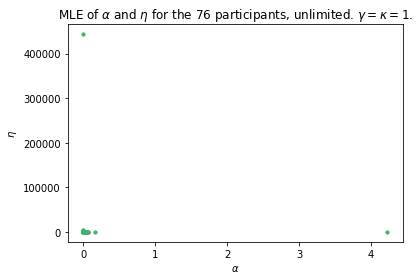
\includegraphics[scale=0.4]{pictures/plotted_mles_unlim_gk1.png}
        \caption[All MLEs plotted, unlimited]{Caption}
        \label{fig:plot_all_mles_unlim_zoom0}
    \end{minipage}\hfill
    \begin{minipage}{0.45\textwidth}
        \centering
        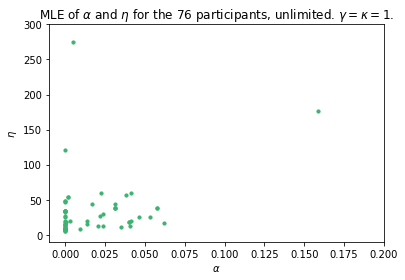
\includegraphics[scale=0.4]{pictures/plotted_mles_unlim_gk1_zoom1.png}
        \caption[Some MLEs plotted, unlimited]{Caption}
        \label{fig:plot_all_mles_unlim_zoom1}
    \end{minipage}
\end{figure}
\end{comment}


\begin{figure}
    \centering
    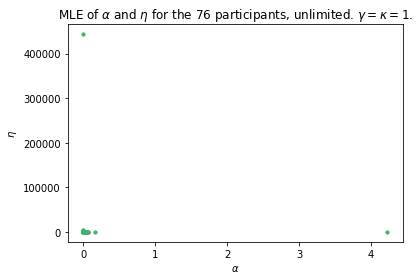
\includegraphics[scale=0.7]{pictures/plotted_mles_unlim_gk1.png}
    \caption[MLEs of $\alpha$ and $\eta$, unlimited with $\gamma=\kappa=1$.]{The MLEs for all the participants plotted for the unlimited case of the box task with $\gamma=\kappa=1$.}
    \label{fig:plot_all_mles_unlim_zoom0}
\end{figure}

\begin{figure}
    \centering
    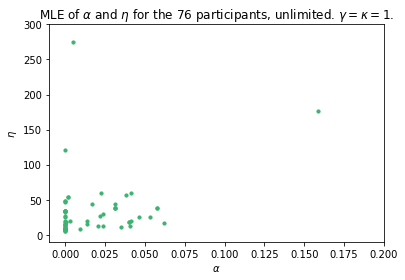
\includegraphics[scale=0.7]{pictures/plotted_mles_unlim_gk1_zoom1.png}
    \caption[MLEs of $\alpha$ and $\eta$, unlimited with $\gamma=\kappa=1$, zoomed.]{The MLEs for all the participants plotted for the unlimited case of the box task with $\gamma=\kappa=1$. Here we have zoomed in closer to zero.}
    \label{fig:plot_all_mles_unlim_zoom1}
\end{figure}

\begin{figure}
    \centering
    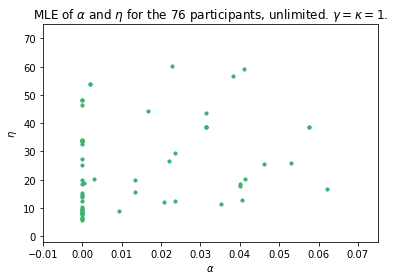
\includegraphics[scale=0.7]{pictures/plotted_mles_unlim_gk1_zoom2.png}
    \caption[MLEs of $\alpha$ and $\eta$, unlimited with $\gamma=\kappa=1$, zoomed more]{The MLEs for all the participants plotted for the unlimited case of the box task with $\gamma=\kappa=1$. Here we have zoomed in closer to zero even more than in Figure \ref{fig:plot_all_mles_unlim_zoom2}.}
    \label{fig:plot_all_mles_unlim_zoom2}
\end{figure}

 

Recall that high values of $\eta$ indicates that the participant makes the decisions with the least expected losses, and $\eta$ is infinity when the participant makes the decisions with the least excepted loss each time a box is opened.  
The log likelihood function is almost flat for high values of $\eta$. That means that the stopping criterion for the optimisation algorithm will be met several places for high values of $\eta$. Thus, if the true value of $\he$ is infinity, we could find that it is for example 10000 because the stopping criterion is met there. We therefore find a threshold for $\eta$ where we can say that all values above that threshold are so high that they go to infinity. Then, we can say that if a participant has $\he$ above that threshold, she always makes the decisions with the least expected loss. This threshold depends on the difference in the two lowest expected losses, but we can for example find one for when the difference is $0.01$.  If we for example have a majority of red boxes, then the expected loss of choosing red as the majority colour is quite low, but so could the expected loss of opening the next box be. Consider, a situation where we have $\EE_0^i(\vp)=0.98$, $\EE_1^i(\vp)=0.02$ and $\EE_2^i(\vp)=0.01$. Then, the decision to open the net box has the lowest expected loss, but the decision to choose red as majority colour is not far away. We then want the threshold value of $\eta$ to so high that the probability that the participant chooses to open the next box is close to one. If $\eta=1000$, the probability that the participant chooses to open the next box given these expected losses, is $0.99995$. Thus, we set $\eta=1000$ as a threshold for when the participant
always makes the choices that have the least expected loss.

 
If we look at the extreme values in Figure \ref{fig:plot_all_mles_unlim_zoom0}, we find one participant with a very high value of $\he$ and small value of $\ha$. This is individual 58, who has MLEs
\begin{equation}
\label{mles_unlim_person58}
    \begin{aligned}
        \ha &= 0.0016,\\
        \he &= 443422.7.
    \end{aligned}
\end{equation}
In each of the three unlimited trials, this individual chooses the majority colour exactly when there are six of one of the colours, which is when we can be completely sure what the true majority colour is. That means that individual 58 chooses after seven boxes are opened in Trial 2, and she then chooses red. In Trials 3 and 4 she chooses after 10 and 9 boxes are opened, respectively. Thus, she always chooses the decision with the least expected loss, which are the decisions an Ideal Observer would make, and $\he$ is therefore above the threshold value of 1000. Individual 58 has $\ha=0.0016$, which is quite small. This might be because she does not open any more boxes than necessary. She might then have a small loss of opening boxes, or some kind of reward of finishing early. This $\ha$ value is so small that it would give an IO solution similar to the one in Figure \ref{fig:unlim_a0.0001_gk1}, such that one always chooses after six boxes of one of the colours have been opened. 

Looking at the other extreme value in Figure \ref{fig:plot_all_mles_unlim_zoom0}, which is individual number 13, we see that she has a high value of $\ha$ and a small value of $\he$. In fact, the value of $\eta$ is negative. The values are
\begin{equation}
\label{mles_unlim_person13}
    \begin{aligned}
        \ha &= 4.2224,\\
        \he &= -0.4290.
    \end{aligned}
\end{equation}
In Trial 2, she chooses after two boxes are opened, where both boxes are red. In both Trial 3 and Trial 4, she chooses when three boxes are opened, where two of them are blue and one is red. She then chooses red as the majority colour despite the fact that choosing blue as the majority colour has a lower expected loss. Thus, she tends to choose the decisions with higher expected losses, and therefore she has a negative estimate of $\eta$. She also chooses quite early, thus she gets a high estimate of $\alpha$. However, an Ideal Observer with this high value of $\alpha$ would always choose after one box is opened.

If we look at a more typical person, we find, for example, individual number 61. She has
\begin{equation}
\label{mles_unilim_person61}
    \begin{aligned}
        \ha &= 0.0135,\\
        \he &= 19.9432.
    \end{aligned}
\end{equation}
In the unlimited trials, she chooses what she thinks is the majority colour after five, six and four boxes are opened. She chooses majority colour before she can be completely sure, and therefore has $\ha>0$. When she chooses however, she chooses the colour with the least expected loss, and thus have a positive $\he$. An IO with the estimates of individual 61 would choose after 3, 10 and 9 boxes were opened, thus her decisions do not coincide with the IO decisions, but they are not far away.  
\begin{figure}
    \centering
    \scalebox{0.7}{
\begin{tikzpicture}[
    treenodeT/.style={
      circle, align=center},
    node distance=1cm,
    ]
    \DoNode{N0-0}{0.58528686868687}{0.58528686868687}{1}{green!70!black}{green!70!black}{0.4};
    \DoNode[below of=N0-0, left of= N0-0]{N1-0}{0.86345353535354}{0.2801202020202}{1}{green!70!black}{green!70!black}{0.4};
    \draw[->] (N0-0) -- (N1-0);
    \DoNode[below of=N0-0, right of= N0-0]{N1-1}{0.2801202020202}{0.86345353535354}{1}{green!70!black}{green!70!black}{0.4};
    \draw[->] (N0-0) -- (N1-1);
    \DoNode[below of=N1-0, left of= N1-0]{N2-0}{0.97258437884379}{0.12018585485855}{1}{green!70!black}{green!70!black}{0.4};
    \draw[->] (N1-0) -- (N2-0);
    \DoNode[below of=N1-0, right of= N1-0]{N2-1}{0.58408986666667}{0.58408986666667}{1}{green!70!black}{green!70!black}{0.4};
    \draw[->] (N1-0) -- (N2-1);
    \draw[->] (N1-1) -- (N2-1);
    \DoNode[below of=N1-1, right of= N1-1]{N2-2}{0.12018585485855}{0.97258437884379}{1}{green!70!black}{green!70!black}{0.4};
    \draw[->] (N1-1) -- (N2-2);
    \DoNode[below of=N2-0, left of= N2-0]{N3-0}{1.00491990407674}{0.04808537170264}{1}{blue}{blue}{0.4};
    \draw[->] (N2-0) -- (N3-0);
    \DoNode[below of=N2-0, right of= N2-0]{N3-1}{0.82258986666667}{0.31858986666667}{1}{green!70!black}{green!70!black}{0.4};
    \draw[->] (N2-0) -- (N3-1);
    \draw[->] (N2-1) -- (N3-1);
    \DoNode[below of=N2-1, right of= N2-1]{N3-2}{0.31858986666667}{0.82258986666667}{1}{green!70!black}{green!70!black}{0.4};
    \draw[->] (N2-1) -- (N3-2);
    \draw[->] (N2-2) -- (N3-2);
    \DoNode[below of=N2-2, right of= N2-2]{N3-3}{0.04808537170264}{1.00491990407674}{1}{red}{red}{0.4};
    \draw[->] (N2-2) -- (N3-3);
    \DoNode[below of=N3-1, left of= N3-1]{N4-1}{0.95401156812339}{0.14424293059126}{1}{green!70!black}{green!70!black}{0.4};
    \draw[->] (N3-1) -- (N4-1);
    \DoNode[below of=N3-1, right of= N3-1]{N4-2}{0.57021468926554}{0.57021468926554}{1}{green!70!black}{green!70!black}{0.4};
    \draw[->] (N3-1) -- (N4-2);
    \draw[->] (N3-2) -- (N4-2);
    \DoNode[below of=N3-2, right of= N3-2]{N4-3}{0.14424293059126}{0.95401156812339}{1}{green!70!black}{green!70!black}{0.4};
    \draw[->] (N3-2) -- (N4-3);
    \DoNode[below of=N4-1, left of= N4-1]{N5-1}{1.0000295202952}{0.05292004920049}{1}{blue}{blue}{0.4};
    \draw[->] (N4-1) -- (N5-1);
    \DoNode[below of=N4-1, right of= N4-1]{N5-2}{0.80388983050847}{0.3095395480226}{1}{green!70!black}{green!70!black}{0.4};
    \draw[->] (N4-1) -- (N5-2);
    \draw[->] (N4-2) -- (N5-2);
    \DoNode[below of=N4-2, right of= N4-2]{N5-3}{0.3095395480226}{0.80388983050847}{1}{green!70!black}{green!70!black}{0.4};
    \draw[->] (N4-2) -- (N5-3);
    \draw[->] (N4-3) -- (N5-3);
    \DoNode[below of=N4-3, right of= N4-3]{N5-4}{0.05292004920049}{1.0000295202952}{1}{red}{red}{0.4};
    \draw[->] (N4-3) -- (N5-4);
    \DoNode[below of=N5-2, left of= N5-2]{N6-2}{0.94858450704225}{0.1269882629108}{1}{green!70!black}{green!70!black}{0.4};
    \draw[->] (N5-2) -- (N6-2);
    \DoNode[below of=N5-2, right of= N5-2]{N6-3}{0.55141489361702}{0.55141489361702}{1}{green!70!black}{green!70!black}{0.4};
    \draw[->] (N5-2) -- (N6-3);
    \draw[->] (N5-3) -- (N6-3);
    \DoNode[below of=N5-3, right of= N5-3]{N6-4}{0.1269882629108}{0.94858450704225}{1}{green!70!black}{green!70!black}{0.4};
    \draw[->] (N5-3) -- (N6-4);
    \DoNode[below of=N6-2, left of= N6-2]{N7-2}{1.00178245614035}{0.0368701754386}{1}{blue}{blue}{0.4};
    \draw[->] (N6-2) -- (N7-2);
    \DoNode[below of=N6-2, right of= N6-2]{N7-3}{0.80387234042553}{0.27195744680851}{1}{green!70!black}{green!70!black}{0.4};
    \draw[->] (N6-2) -- (N7-3);
    \draw[->] (N6-3) -- (N7-3);
    \DoNode[below of=N6-3, right of= N6-3]{N7-4}{0.27195744680851}{0.80387234042553}{1}{green!70!black}{green!70!black}{0.4};
    \draw[->] (N6-3) -- (N7-4);
    \draw[->] (N6-4) -- (N7-4);
    \DoNode[below of=N6-4, right of= N6-4]{N7-5}{0.0368701754386}{1.00178245614035}{1}{red}{red}{0.4};
    \draw[->] (N6-4) -- (N7-5);
    \DoNode[below of=N7-3, left of= N7-3]{N8-3}{0.96071176470588}{0.07835882352941}{1}{green!70!black}{green!70!black}{0.4};
    \draw[->] (N7-3) -- (N8-3);
    \DoNode[below of=N7-3, right of= N7-3]{N8-4}{0.53182142857143}{0.53182142857143}{1}{green!70!black}{green!70!black}{0.4};
    \draw[->] (N7-3) -- (N8-4);
    \draw[->] (N7-4) -- (N8-4);
    \DoNode[below of=N7-4, right of= N7-4]{N8-5}{0.07835882352941}{0.96071176470588}{1}{green!70!black}{green!70!black}{0.4};
    \draw[->] (N7-4) -- (N8-5);
    \DoNode[below of=N8-3, left of= N8-3]{N9-3}{1.0135}{0.0135}{1}{blue}{blue}{0.4};
    \draw[->] (N8-3) -- (N9-3);
    \DoNode[below of=N8-3, right of= N8-3]{N9-4}{0.83975}{0.19689285714286}{1}{green!70!black}{green!70!black}{0.4};
    \draw[->] (N8-3) -- (N9-4);
    \draw[->] (N8-4) -- (N9-4);
    \DoNode[below of=N8-4, right of= N8-4]{N9-5}{0.19689285714286}{0.83975}{1}{green!70!black}{green!70!black}{0.4};
    \draw[->] (N8-4) -- (N9-5);
    \draw[->] (N8-5) -- (N9-5);
    \DoNode[below of=N8-5, right of= N8-5]{N9-6}{0.0135}{1.0135}{1}{red}{red}{0.4};
    \draw[->] (N8-5) -- (N9-6);
    \DoNode[below of=N9-4, left of= N9-4]{N10-4}{1.0135}{0.0135}{1}{blue}{blue}{0.4};
    \draw[->] (N9-4) -- (N10-4);
    \DoNode[below of=N9-4, right of= N9-4]{N10-5}{0.5135}{0.5135}{1}{green!70!black}{green!70!black}{0.4};
    \draw[->] (N9-4) -- (N10-5);
    \draw[->] (N9-5) -- (N10-5);
    \DoNode[below of=N9-5, right of= N9-5]{N10-6}{0.0135}{1.0135}{1}{red}{red}{0.4};
    \draw[->] (N9-5) -- (N10-6);
    \DoNode[below of=N10-5, left of= N10-5]{N11-5}{1.0135}{0.0135}{1}{blue}{blue}{0.4};
    \draw[->] (N10-5) -- (N11-5);
    \DoNode[below of=N10-5, right of= N10-5]{N11-6}{0.0135}{1.0135}{1}{red}{red}{0.4};
    \draw[->] (N10-5) -- (N11-6);
    
\end{tikzpicture}
}
    \caption[Ideal Observer solution individual 61, unlimited. $\gamma=\kappa=1$]{Here we see and Ideal Observer solution of the box task in the unlimited case for individual number 61 with a uniform prior, such that $\gamma=\kappa=1$. She has $\ha=0.0135$. This tree can be interpreted in the same way as the tree in Figure \ref{fig:unlim_a0.0001_gk1}.}
    \label{fig:IO_sol_individual61}
\end{figure}

Having looked at the MLEs in the unlimited case, we now continue with the limited trials. 


\subsubsection{Limited}
In the limited version, we have three parameters, $\alpha$, $\beta$ and $\eta$, and we have found maximum likelihood estimates for these for all of the 76 participants. The MLEs of $\alpha$ and $\eta$ for all participants are plotted in Figure \ref{fig:mles_limited_alpha_eta}, and we have zoomed in on that plot in Figure \ref{fig:mles_limited_alpha_eta_zoomed}. We see that many of the participants have $\hat{\alpha}=0$. In fact, all participants except four have $\ha=0$. We also see that four of the participants have $\he$ higher than the threshold value of 1000, meaning that they make good choices each time a box is opened. What is not so easy to see is that the two participants with the highest values of $\ha$ have negative values of $\he$. This indicates that they make choices with high expected losses and that they have high costs of opening new boxes. 
\begin{figure}
    \centering
    \begin{minipage}{0.48\textwidth}
        \centering
        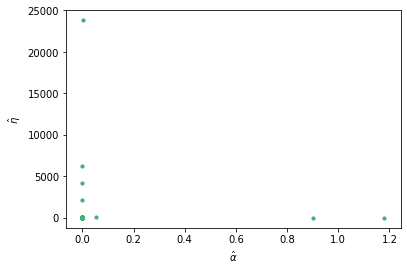
\includegraphics[scale=0.38]{pictures/plotted_mles_limited_alpha_eta_gk1.png}
        \caption[MLEs of $\alpha$ and $\eta$, limited. $\gamma=\kappa=1$]{Maximum likelihood estimates of $\alpha$ and $\eta$ for all participants in the limited version of the box task. $\gamma=\kappa=1$.}
        \label{fig:mles_limited_alpha_eta}
    \end{minipage}\hfill
    \begin{minipage}{0.48\textwidth}
        \centering
        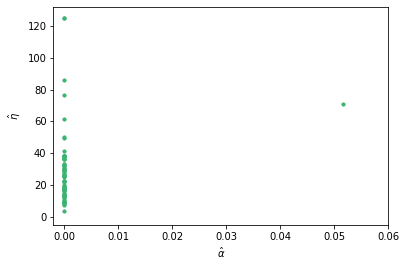
\includegraphics[scale=0.38]{pictures/plotted_mles_limited_alpha_eta_gk1_zoomed.png}
        \caption[MLEs of $\alpha$ and $\eta$ zoomed, limited. $\gamma=\kappa=1$]{MLEs of $\alpha$ and $\eta$ in the limited case. Zoomed in on the plot in Figure \ref{fig:mles_limited_alpha_eta}.}
        \label{fig:mles_limited_alpha_eta_zoomed}
    \end{minipage}
\end{figure}

In Figure \ref{fig:mles_limited_alpha_beta} we have plotted the MLEs of $\alpha$ and $\beta$ for all participants. Again we see that many participants have $\ha=0$. This might indicate that $\alpha$ is unnecessary to include in the limited version. Both $\alpha$ and $\beta$ are values tied to whether we choose majority colour early or not. Thus, it might be enough to only include $\beta$. It is also not obvious how the MLEs are giving weight to $\alpha$ compared to $\beta$. 
\begin{figure}
    \centering
    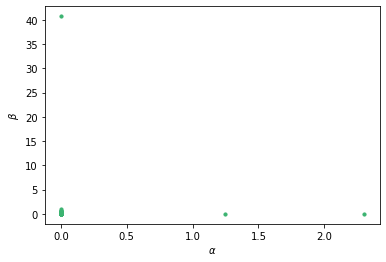
\includegraphics[scale=0.38]{pictures/plotted_mles_limited_alpha_beta_gk1.png}
    \caption[MLEs of $\alpha$ and $\beta$, limited. $\gamma=\kappa=1$]{Maximum likelihood estimates of $\alpha$ and $\beta$ for all participants in the limited version of the box task.$\gamma=\kappa=1$.}
    \label{fig:mles_limited_alpha_beta}
\end{figure}



We have also plotted the MLEs of $\beta$ and $\eta$ together in Figure \ref{fig:mles_limited_beta_eta}. Again we see that four of the participants have high values of $\he$. Three of these have values of $\hb$ close to one, which might indicate that they are afraid of the test terminating, and thus choose early, but that they choose the colour that is most likely to be in majority. Zooming in on the plot as in Figure \ref{fig:mles_limited_beta_eta_zoomed}, we see that the majority of the participants have $\he$ values between 10 and 80 and $\hb$ values between zero and 0.7. We also see that some participants have $\hb$ equal to zero. 
\begin{figure}
    \centering
    \begin{minipage}{0.48\textwidth}
        \centering
        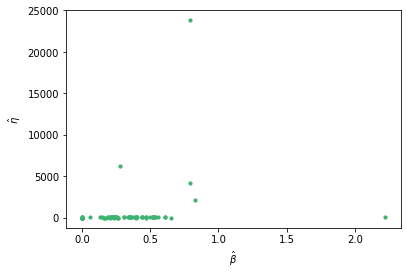
\includegraphics[scale=0.38]{pictures/plotted_mles_limited_beta_eta_gk1.png}
        \caption[MLEs of $\beta$ and $\eta$, limited. $\gamma=\kappa=1$]{Maximum likelihood estimates of $\beta$ and $\eta$ for all participants in the limited version of the box task. $\gamma=\kappa=1$.}
        \label{fig:mles_limited_beta_eta}
    \end{minipage}
    \hfill
    \begin{minipage}{0.48\textwidth}
        \centering
        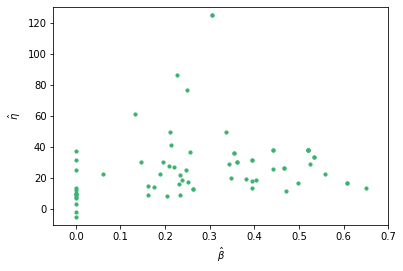
\includegraphics[scale=0.38]{pictures/plotted_mles_limited_beta_eta_zoomed_gk1.png}
        \caption[MLEs of $\beta$ and $\eta$ zoomed, limited. $\gamma=\kappa=1$]{MLEs of $\beta$ and $\eta$ in the limited case. Zoomed in on the plot in Figure \ref{fig:mles_limited_beta_eta}.}
        \label{fig:mles_limited_beta_eta_zoomed}
    \end{minipage}
\end{figure}


In Figures \ref{fig:mles_limited_alpha_eta} and \ref{fig:mles_limited_beta_eta} we see a participant with a very high value of $\he$. This is individual number 70, and she has  parameter estimates
\begin{equation}
\label{mles_lim_person70}
    \begin{aligned}
        \ha &= 0.0015,\\
        \hb &= 0.7929,\\
        \he &= 23851.9.
    \end{aligned}
\end{equation}
She chooses what she thinks is the majority colour after either two or three boxes are opened in the limited trials. When there are two boxes of the same colour, she chooses that colour as the majority colour. In Figure \ref{fig:IO_sol_person_70} we see the Ideal Observer solution for an individual with the values given in \eqref{mles_lim_person70}. We see that the IO would do the exact same thing as individual number 70 has done, that is, choose when we have two boxes of the same colour, and then choose that colour as the dominant colour. In Trial 5 that is after two boxes are opened as the first two boxes are blue. This is visualised in Figure \ref{fig:IO_sol_perosn_70_trial5}. In Trial 6 both the IO and participant number 70 chooses after three boxes are opened as seen in Figure \ref{fig:IO_sol_person70_trial6}.
\begin{figure}
    \centering
    \scalebox{0.7}{
\begin{tikzpicture}[
    treenodeT/.style={
      circle, align=center},
    node distance=1cm,
    ]
    \DoNode{N0-0}{0.7082286271809}{0.7082286271809}{1}{green!70!black}{green!70!black}{0.4};
    \DoNode[below of=N0-0, left of= N0-0]{N1-0}{0.99839529384757}{0.41506196051423}{1}{green!70!black}{green!70!black}{0.4};
    \draw[->] (N0-0) -- (N1-0);
    \DoNode[below of=N0-0, right of= N0-0]{N1-1}{0.41506196051423}{0.99839529384757}{1}{green!70!black}{green!70!black}{0.4};
    \draw[->] (N0-0) -- (N1-1);
    \DoNode[below of=N1-0, left of= N1-0]{N2-0}{1.07340992619926}{0.22101140221402}{1}{blue}{blue}{0.4};
    \draw[->] (N1-0) -- (N2-0);
    \DoNode[below of=N1-0, right of= N1-0]{N2-1}{0.80399}{0.80399}{1}{green!70!black}{green!70!black}{0.4};
    \draw[->] (N1-0) -- (N2-1);
    \draw[->] (N1-1) -- (N2-1);
    \DoNode[below of=N1-1, right of= N1-1]{N2-2}{0.22101140221402}{1.07340992619926}{1}{red}{red}{0.4};
    \draw[->] (N1-1) -- (N2-2);
    \DoNode[below of=N2-1, left of= N2-1]{N3-1}{1.00224410074074}{0.49824410074074}{1}{blue}{blue}{0.4};
    \draw[->] (N2-1) -- (N3-1);
    \DoNode[below of=N2-1, right of= N2-1]{N3-2}{0.49824410074074}{1.00224410074074}{1}{red}{red}{0.4};
    \draw[->] (N2-1) -- (N3-2);
    
\end{tikzpicture}
}
    \caption[Ideal Observer solution individual 70, limited. $\gamma=\kappa=1$]{An Ideal Observer solution for individual number 70 in the limited version of the box task with $\gamma=\kappa=1$.}
    \label{fig:IO_sol_person_70}
\end{figure}

\begin{figure}
    \centering
    \begin{minipage}{0.48\textwidth}
        \centering
        \scalebox{0.7}{\begin{tikzpicture}[
    treenodeT/.style={
      circle, align=center},
    node distance=1cm,
    ]
    \DoNode{N0-0}{0.7082286271809}{0.7082286271809}{1}{green!70!black}{green!70!black}{0.4};
    \DoNode[below of=N0-0, left of= N0-0]{N1-0}{0.99839529384757}{0.41506196051423}{1}{green!70!black}{green!70!black}{0.4};
    \draw[->] (N0-0) -- (N1-0);
    \DoNodePale[below of=N0-0, right of= N0-0]{N1-1}{0.41506196051423}{0.99839529384757}{1}{green!70!black}{green!70!black}{0.4};
    \draw[->,black!10] (N0-0) -- (N1-1);
    \DoNode[below of=N1-0, left of= N1-0]{N2-0}{1.07340992619926}{0.22101140221402}{1}{blue}{blue}{0.4};
    \draw[->] (N1-0) -- (N2-0);
    \DoNodePale[below of=N1-0, right of= N1-0]{N2-1}{0.80399}{0.80399}{1}{green!70!black}{green!70!black}{0.4};
    \draw[->,black!10] (N1-0) -- (N2-1);
    \draw[->,black!10] (N1-1) -- (N2-1);
    \DoNodePale[below of=N1-1, right of= N1-1]{N2-2}{0.22101140221402}{1.07340992619926}{1}{red}{red}{0.4};
    \draw[->,black!10] (N1-1) -- (N2-2);
    \DoNodePale[below of=N2-1, left of= N2-1]{N3-1}{1.00224410074074}{0.49824410074074}{1}{blue}{blue}{0.4};
    \draw[->,black!10] (N2-1) -- (N3-1);
    \DoNodePale[below of=N2-1, right of= N2-1]{N3-2}{0.49824410074074}{1.00224410074074}{1}{red}{red}{0.4};
    \draw[->,black!10] (N2-1) -- (N3-2);
    
\end{tikzpicture}
}
        \caption[Ideal Observer solution individual 70 in trial 5. $\gamma=\kappa=1$]{An Ideal Observer solution of Trial 5 for individual number 70 where $\gamma=\kappa=1$.}
        \label{fig:IO_sol_perosn_70_trial5}
    \end{minipage}
    \hfill
    \begin{minipage}{0.48\textwidth}
        \centering
        \scalebox{0.7}{\begin{tikzpicture}[
    treenodeT/.style={
      circle, align=center},
    node distance=1cm,
    ]
    \DoNode{N0-0}{0.7082286271809}{0.7082286271809}{1}{green!70!black}{green!70!black}{0.4};
    \DoNodePale[below of=N0-0, left of= N0-0]{N1-0}{0.99839529384757}{0.41506196051423}{1}{green!70!black}{green!70!black}{0.4};
    \draw[->,black!10] (N0-0) -- (N1-0);
    \DoNode[below of=N0-0, right of= N0-0]{N1-1}{0.41506196051423}{0.99839529384757}{1}{green!70!black}{green!70!black}{0.4};
    \draw[->] (N0-0) -- (N1-1);
    \DoNodePale[below of=N1-0, left of= N1-0]{N2-0}{1.07340992619926}{0.22101140221402}{1}{blue}{blue}{0.4};
    \draw[->,black!10] (N1-0) -- (N2-0);
    \DoNode[below of=N1-0, right of= N1-0]{N2-1}{0.80399}{0.80399}{1}{green!70!black}{green!70!black}{0.4};
    \draw[->,black!10] (N1-0) -- (N2-1);
    \draw[->] (N1-1) -- (N2-1);
    \DoNodePale[below of=N1-1, right of= N1-1]{N2-2}{0.22101140221402}{1.07340992619926}{1}{red}{red}{0.4};
    \draw[->,black!10] (N1-1) -- (N2-2);
    \DoNode[below of=N2-1, left of= N2-1]{N3-1}{1.00224410074074}{0.49824410074074}{1}{blue}{blue}{0.4};
    \draw[->] (N2-1) -- (N3-1);
    \DoNodePale[below of=N2-1, right of= N2-1]{N3-2}{0.49824410074074}{1.00224410074074}{1}{red}{red}{0.4};
    \draw[->,black!10] (N2-1) -- (N3-2);
    
\end{tikzpicture}
}
        \caption[Ideal Observer solution individual 70 in trial 6. $\gamma=\kappa=1$]{An Ideal Observer solution of Trial 6 for individual number 70 where $\gamma=\kappa=1$.}
        \label{fig:IO_sol_person70_trial6}
    \end{minipage}
\end{figure}

We have two individuals with high values of $\ha$. They both have $\hb=0$ and negative values of $\he$. These two individuals can be interpreted the same way, and we therefore present only the participant with the highest $\ha$ here. This is individual number 11. Her parameter estimates are
\begin{equation}
\label{mles_lim_person11}
    \begin{aligned}
        \ha &= 1.1798,\\
        \hb &= 0.0,\\
        \he &= -1.9538.
    \end{aligned}
\end{equation}
She chooses after two or three boxes are opened, and she tends to choose the colour that is in minority, not majority, out of the opened boxes. This is the reason for $\he$ being negative. $\hb$ is a measure of the loss one gets when the test terminates. If the test terminates, this counts as a failed trial. It also counts as a failed trial if the participant chooses the wrong colour as the majority colour. This individual does not seem to care if she chooses the wrong colour as the majority colour, and we might believe that, in the same way, she does not care whether the test terminates or not. This might be the reason that $\hb$ is zero. However, as she chooses after two and three boxes are opened, this indicates some kind of loss of opening boxes, thus we get the high value of $\ha$. 
Earlier, we discussed that $\alpha$ might be unnecessary in the limited trials as so many participants have $\ha=0$. However, for individual number 11 and the other participant with the high value of $\ha$, this parameter might be needed to express some kind of penalty of opening boxes as we have that $\hb=0$.
In Figure \ref{fig:IO_sol_person11_limited_gk1} we see that an Ideal Observer with the same estimates as individual number 11 would choose majority colour before any boxes are opened. The expected loss of choosing majority colour then is 0.5 as it is the probability that the opposite colour is in majority. The expected loss of opening the first box is much higher due to the high value of $\ha$. 
\begin{figure}
    \centering
    \scalebox{0.7}{
\begin{tikzpicture}[
    treenodeT/.style={
      circle, align=center},
    node distance=1cm,
    ]
    \DoNode{N0-0}{1.88813333333333}{1.88813333333333}{1}{blue}{red}{0.4};
    
\end{tikzpicture}
}
    \caption[Ideal Observer solution individual 11, limited. $\gamma=\kappa=1$]{An Ideal Observer solution for individual number 13 in the limited version of the box task with $\gamma=\kappa=1$.}
    \label{fig:IO_sol_person11_limited_gk1}
\end{figure}


In Figures \ref{fig:mles_limited_alpha_beta} and \ref{fig:mles_limited_beta_eta} we see participant number 75 that has a high value of $\hb$. Her parameter estimates are
\begin{equation}
\label{mles_lim_person75}
    \begin{aligned}
        \ha &= 0.0517,\\
        \hb &= 2.219,\\
        \he &= 70.87.
    \end{aligned}
\end{equation}
This participant chooses after one box is opened in all of the six limited trials, hence, the high value of $\hb$. At the same time, individual 75 always chooses the colour of that first box as the majority colour, which is the colour with the least expected loss. The expected loss of opening the next box might be lower than the expected loss of choosing that as the majority colour. However, these expected losses are often close to each other, whereas the expected loss of choosing the other colour as the majority is often further away. Thus, she tends to choose decisions with low expected losses, but they might not be the decisions with the lowest expected loss. The value of $\he$ is therefore quite high.
%, but not so high that it reaches the threshold value for $\eta$. However, that threshold value is based on expected losses that differ in value with $0.01$. Here, the expected losses differ more as the parameter estimates are quite high. Thus, the threshold value of $\eta$ might be a lot smaller in this situation. 

If we look at a more typical person, we find, for example, individual number 40. She has parameter estimates
\begin{equation}
\label{mles_lim_person40}
    \begin{aligned}
        \ha &= 0.0,\\
        \hb &= 0.4414,\\
        \he &= 38.00.
    \end{aligned}
\end{equation}
She opens between 2 and 5 boxes in all the trials except Trial 8. In all of these trials she chooses the most probable colour as the colour that she believes is the majority colour. Thus, $\he$ is reasonably high. In Trial 8 she opens nine boxes and tries to open the tenth when the test terminates. In that trial there are never two boxes of the same colour that is opened after each other, and the probability that one of the colours is the majority colour is quite low. 









\subsection{Confidence Intervals}
\label{chapter:results_cis}
We have presented an Ideal Observer solution of the box task and the maximum likelihood estimates for different participants. Now, we will discuss some of the confidence intervals we have found. Recall that these are found by finding the MLEs of 1000 bootstrap samples for each participant and the finding the 5-th and 95-th percentiles, as discussed in Chapter \ref{chapter:CIs_chap3}. 

\subsubsection{Unlimited}
We start with the confidence intervals in the unlimited case. In Figure \ref{fig:all_cis_alpha_unlim_v2} we see the confidence intervals for $\alpha$. The whole interval for individual number 13 is not included as it is very long. Recall that the MLE of $\alpha$ for person 13 is very large, and we also have a very large value of the upper limit of the CI for $\alpha$, $\ha_{1000}^{(95)}$. We see that many of the CIs include zero, meaning that many participants might not have that small loss of opening the next box. 
\begin{figure}
    \centering
    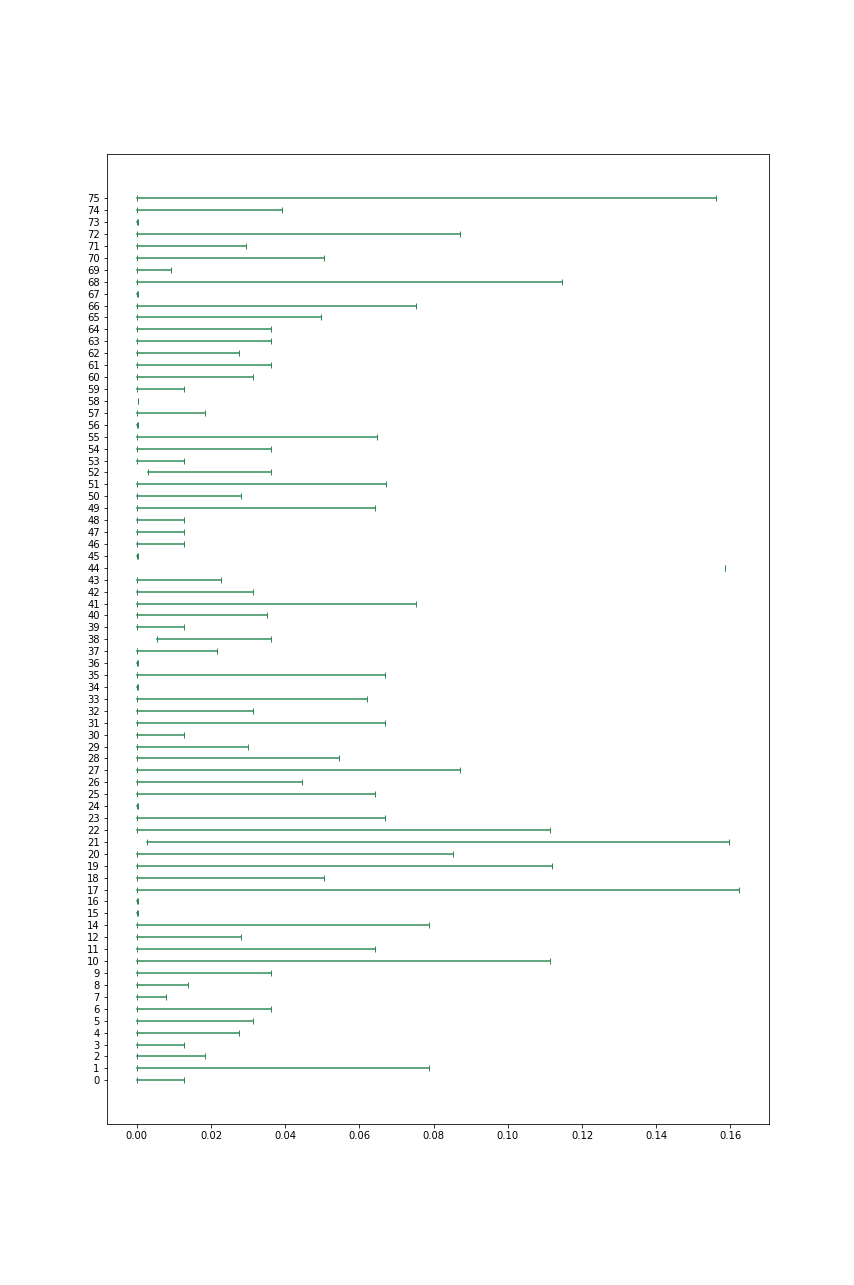
\includegraphics[scale=0.37]{pictures/all_cis_unlim_alpha.png}
    \caption[CIs for $\alpha$, unlimited. $\gamma=\kappa=1$]{Here are the confidence intervals for all the participants for $\alpha$ in the unlimited version of the box task. We see that individual number 13 has an interval outside the range of this plot. $\gamma=\kappa=1$.}
    \label{fig:all_cis_alpha_unlim_v2}
\end{figure}



In Figure \ref{fig:all_cis_eta_unlim_v2} we see all the CIs in the unlimited case for $\eta$. We see that some of the participants have the whole CI above 1000, the threshold value we defined for $\he$. We can for these participants conclude that they always make decisions with small expected losses. We also see that many of the CIs include the threshold value. In Figure \ref{fig:all_cis_eta_unlim_zoomed} we have zoomed in on the CIs, and added a line at zero. Only one CI include zero, the CI for individual number 13. Recall that she has a negative value of $\he$ and a very high $\ha$.
\begin{figure}
    \centering
    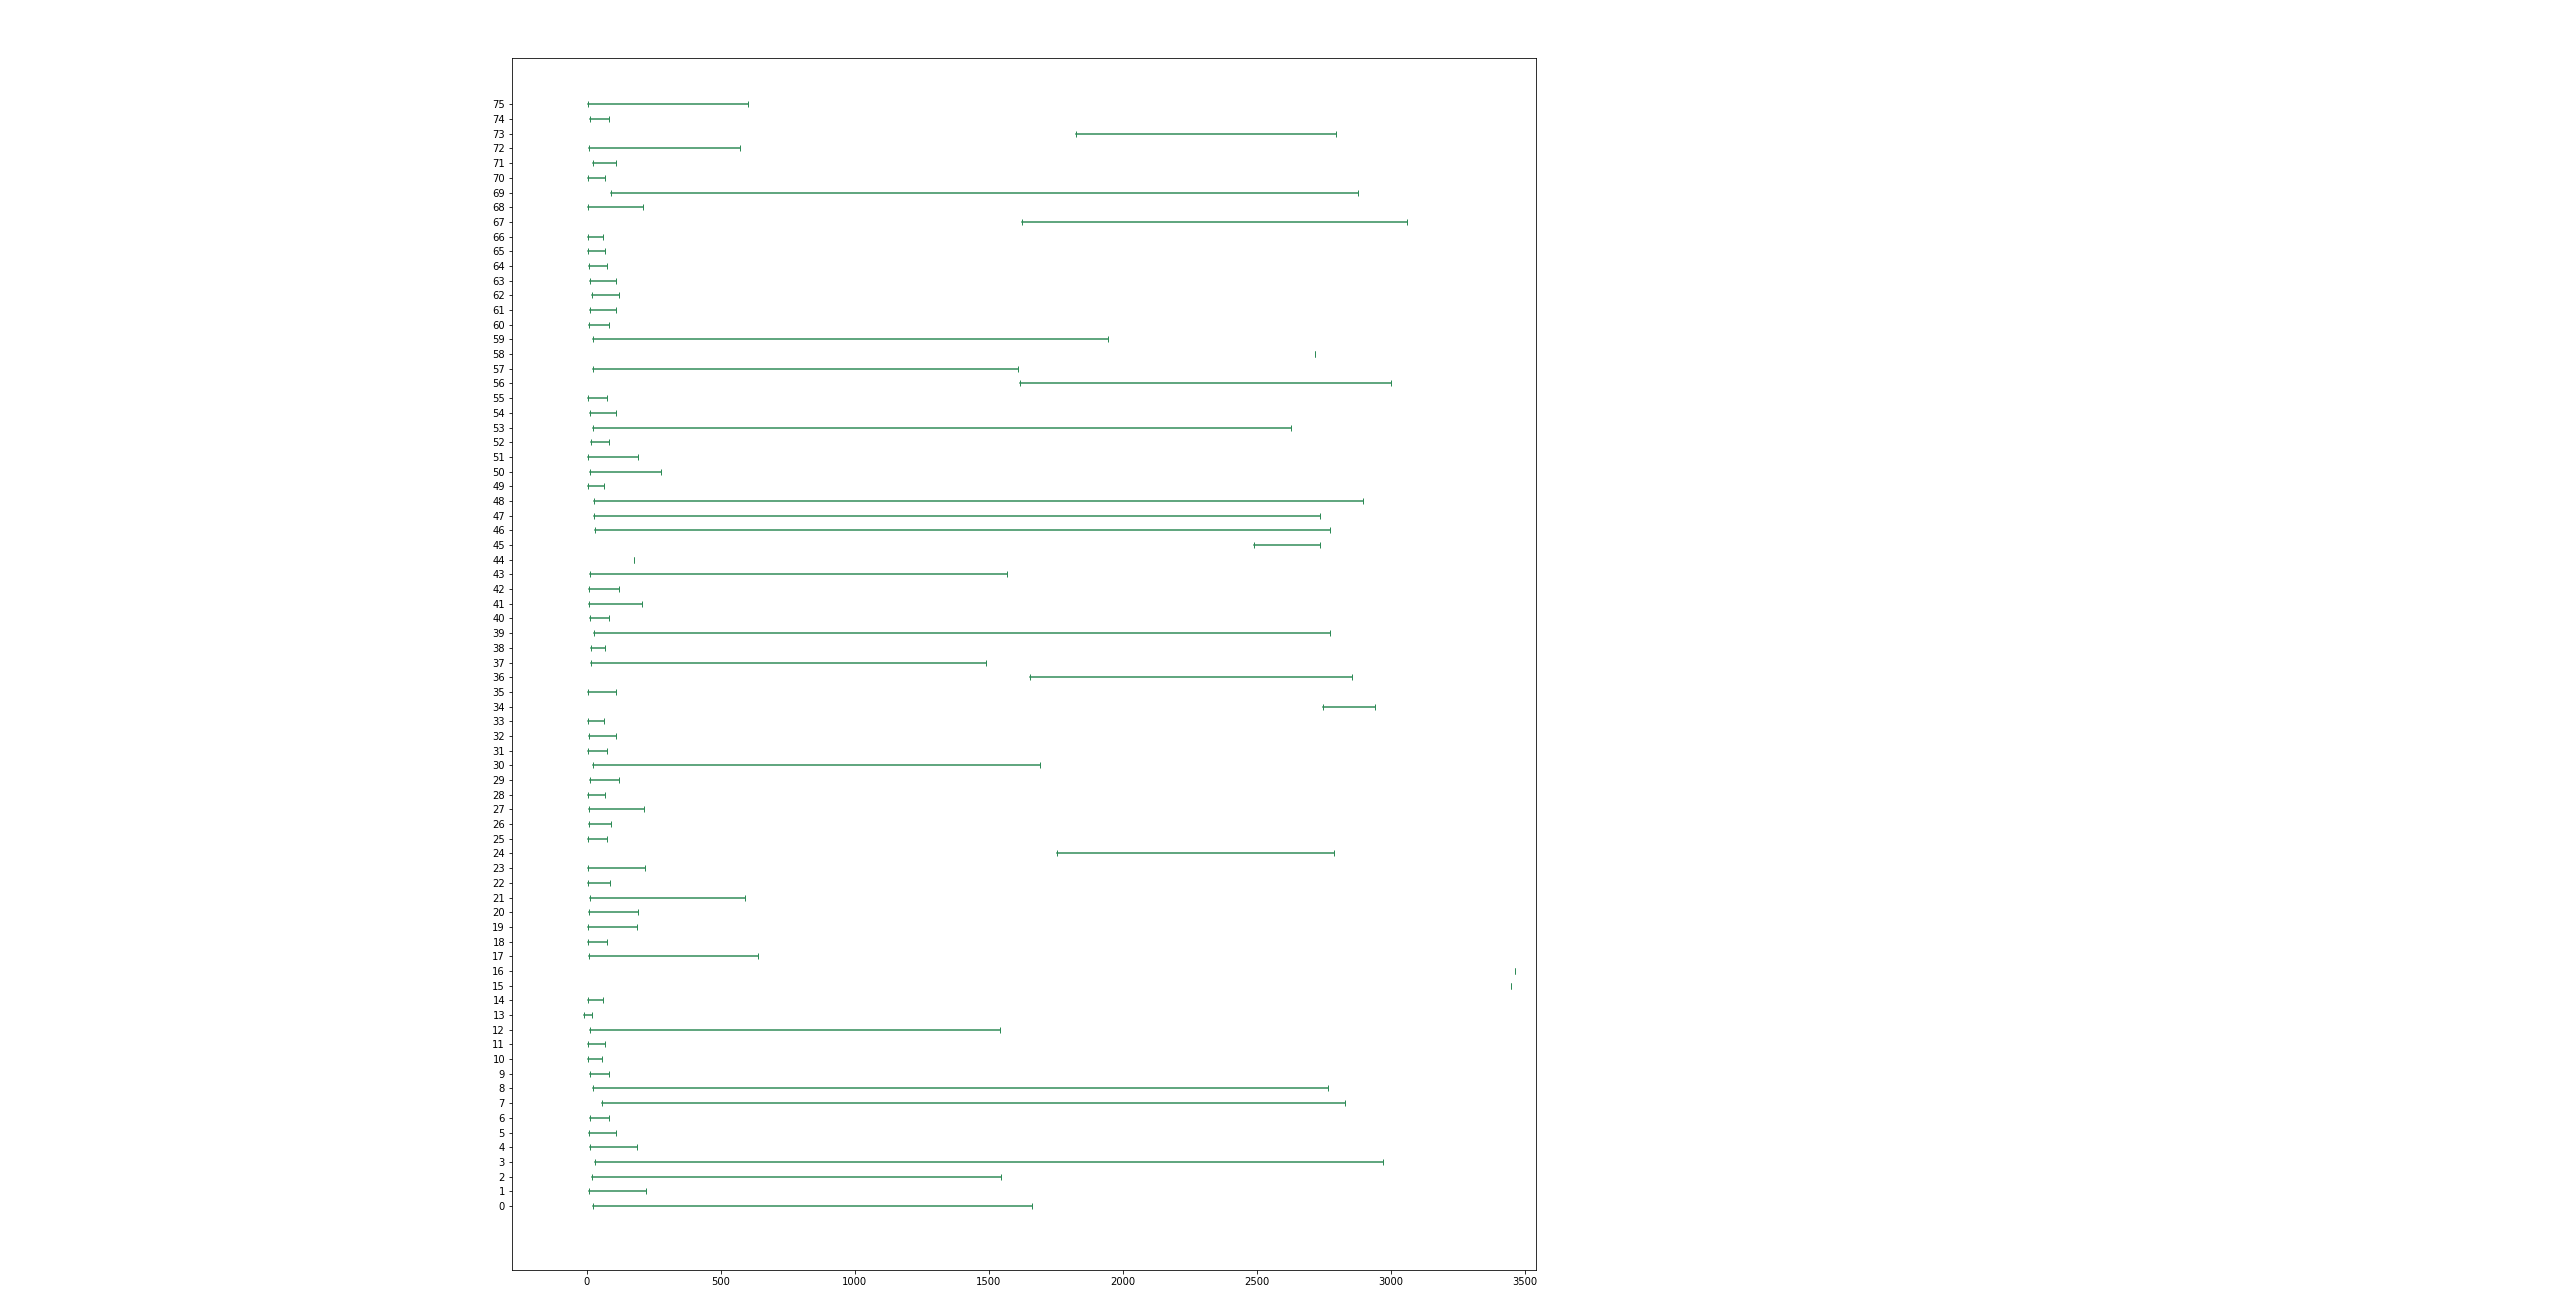
\includegraphics[scale=0.38]{pictures/test_cis_eta_unlim.png}
    \caption[CIs for $\eta$, unlimited. $\gamma=\kappa=1$]{Confidence intervals for each participant for $\eta$ in the unlimited version of the box task. $\gamma=\kappa=1$.}
    \label{fig:all_cis_eta_unlim_v2}
\end{figure}

\begin{figure}
    \centering
    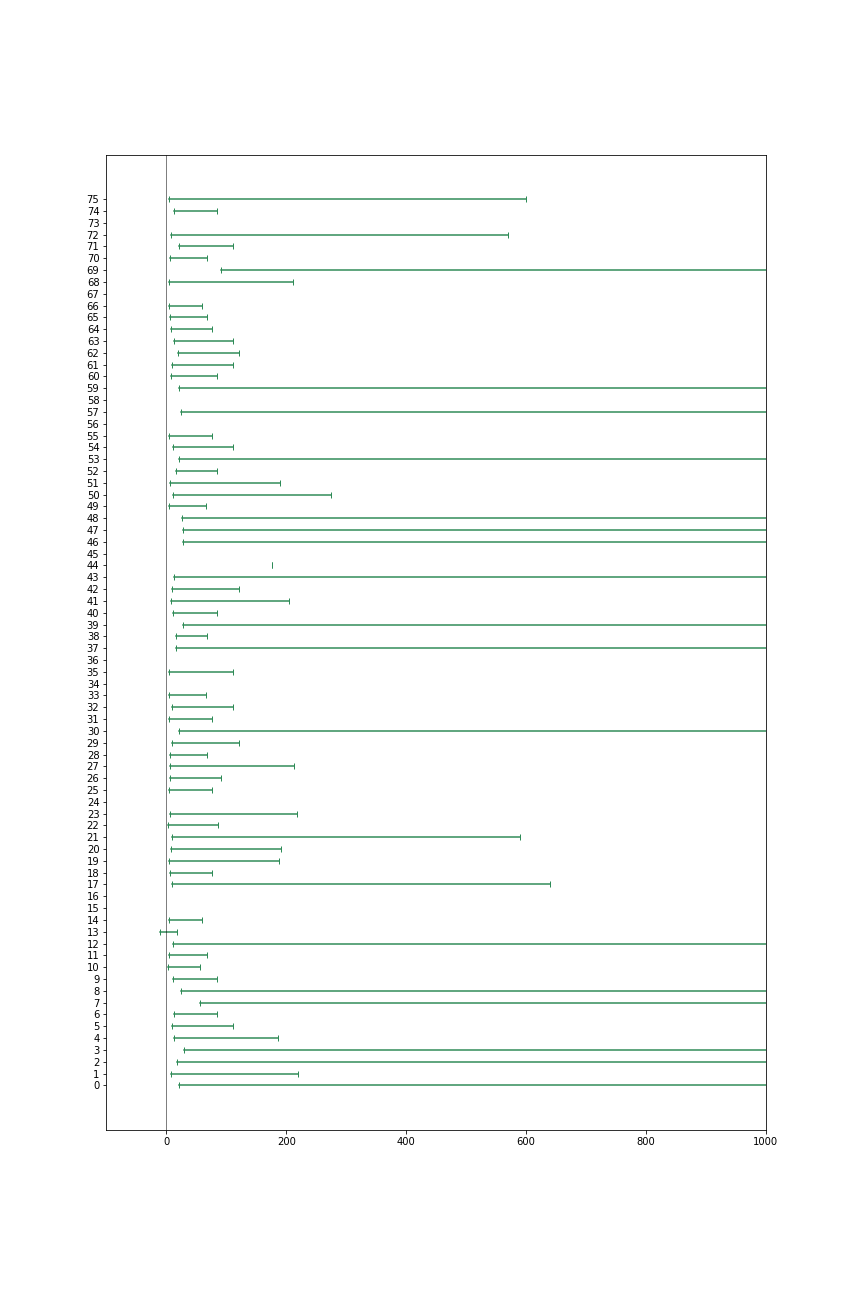
\includegraphics[scale=0.38]{pictures/all_cis_unlim_eta_zoomed.png}
    \caption[CIs for $\eta$ zoomed, unlimited. $\gamma=\kappa=1$]{Confidence intervals of $\eta$ for each participant in the unlimited trials of the box task with $\gamma=\kappa=1$, zoomed.}
    \label{fig:all_cis_eta_unlim_zoomed}
\end{figure}


In Chapter \ref{chapter:mles} we discussed individual 61 that has MLEs in the middle of the range of the MLEs. The MLEs are as given in \eqref{mles_unilim_person61}.
We have 1000 bootstrap samples and thus 1000 values of both $\hat{\alpha}$ and $\he$ for this participant. These are plotted in Figure \ref{fig:ci_unlim_person_61}. There, we have also plotted the confidence interval as black lines. We see that most of the bootstrap samples are accumulated in the bottom left corner. Thus, we zoom in there in Figure \ref{fig:ci_unlim_person_61_zoomed}, where we also have plotted the CI. We have that
\begin{equation*}
    [\hat{\alpha}^{*(5)}_{1000},\hat{\alpha}^{*(95)}_{1000}] = [0,0.0362]
\end{equation*}
and
\begin{equation*}
    [\hat{\eta}^{*(5)}_{1000},\hat{\eta}^{*(95)}_{1000}] = [10.0449,110.3661].
\end{equation*}
We see that the confidence interval for $\alpha$ includes zero. Recall that having $\ha=0$ means that one does not have any cost of opening boxes. Additionally, we see that the whole interval for $\eta$ is above zero, which means that individual number 61 makes decisions with low expected losses, although they might not always be the decisions with the lowest expected loss. 


\begin{figure}
    \centering
    \begin{minipage}{0.48\textwidth}
        \centering
        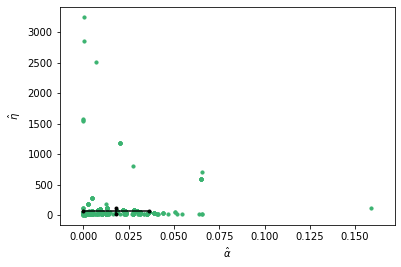
\includegraphics[scale=0.37]{pictures/ci_unlim_person61.png}
        \caption[MLEs of bootstrap samples individual 61, unlimited]{All of the MLEs of the 1000 bootstrap samples plotted for individual number 61 in the unlimited case with $\gamma=\kappa=1$. The confidence intervals for the two parameters are also included.}
        \label{fig:ci_unlim_person_61}
    \end{minipage}\hfill
    \begin{minipage}{0.48\textwidth}
        \centering
        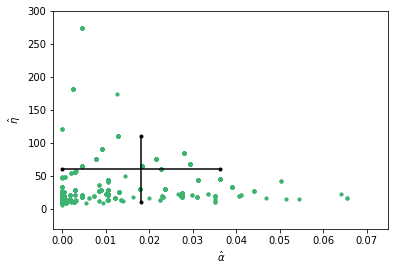
\includegraphics[scale=0.37]{pictures/ci_unlim_person61_zoomed.png}
        \caption[MLEs of bootstrap samples individual 61, unlimited, zoomed]{Here we have zoomed in on the bootstrap samples and confidence intervals that are plotted in Figure \ref{fig:ci_unlim_person_61}. This is for individual number 61 in the unlimited case with $\gamma=\kappa=1$.}
        \label{fig:ci_unlim_person_61_zoomed}
    \end{minipage}
\end{figure}

In Chapter \ref{chapter:mles} we also discussed individual number 13 that has a high $\ha$, as seen in \eqref{mles_unlim_person13}, compared to the other participants. The 1000 bootstrap samples for participant number 13 are plotted in Figure \ref{fig:ci_unlim_person_13}, and zoomed on the $\he$ axis in Figure \ref{fig:ci_unlim_person_13_zoomed}. The CIs are
\begin{equation*}
    [\hat{\alpha}^{*(5)}_{1000},\hat{\alpha}^{*(95)}_{1000}] = [0,1246.3510]
\end{equation*}
and
\begin{equation*}
    [\hat{\eta}^{*(5)}_{1000},\hat{\eta}^{*(95)}_{1000}] = [-9.9272,18.3986].
\end{equation*}
We see that many of the values of $\ha$ are very high, much higher than the MLE, thus $\hat{\alpha}^{*(95)}_{1000}$ is very high. That means that the estimates for this individual are uncertain. Thus, the model might not be a good fit for this participant and the choices she makes. This might be because the expected loss are based on the next decisions that will be made. We have decided that these decisions are the decisions that an Ideal Observer would make, the decisions with the least expected losses. However, this participant tends to make decisions with high expected losses, meaning that the decisions we include in the model are not so relevant for this individual. Thus, we might conclude that this model is not a great fit for participants that make decisions with high expected losses. 
\begin{figure}
    \centering
    \begin{minipage}{0.48\textwidth}
        \centering
        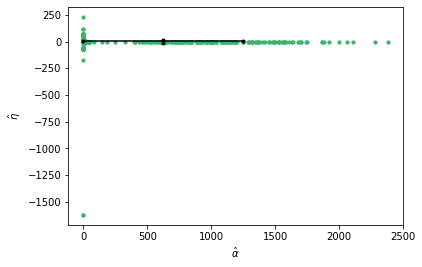
\includegraphics[scale=0.37]{pictures/ci_unlim_person13.png}
        \caption[MLEs of bootstrap samples individual 13, unlimited]{All of the MLEs of the 1000 bootstrap samples plotted for individual number 13 in the unlimited case with $\gamma=\kappa=1$. The confidence intervals for the two parameters are also included.}
        \label{fig:ci_unlim_person_13}
    \end{minipage}\hfill
    \begin{minipage}{0.48\textwidth}
        \centering
        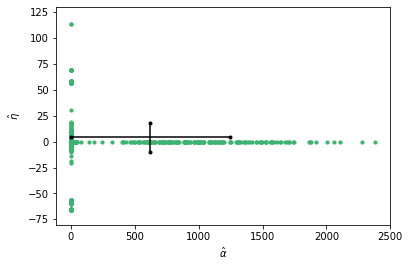
\includegraphics[scale=0.37]{pictures/ci_unlim_person13_zoomed.png}
        \caption[MLEs of bootstrap samples individual 13, unlimited, zoomed]{Here we have zoomed in on the bootstrap samples and confidence intervals that are plotted in Figure \ref{fig:ci_unlim_person_61}. This is for individual number 13 in the unlimited case with $\gamma=\kappa=1$.}
        \label{fig:ci_unlim_person_13_zoomed}
    \end{minipage}
\end{figure}
%commenting out figure where zooming even more for person 13. 
\begin{comment}
\begin{figure}
    \centering
    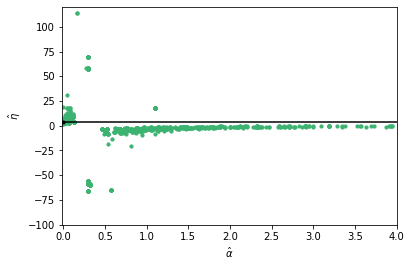
\includegraphics[scale=0.7]{pictures/ci_unlim_person13_zoomed2.png}
    \caption{ci unlim person 13 zoomed even more. Kanskje ikke zoome såå mye siden mle er på4.2???}
    \label{fig:ci_unlim_person_13_zoomed2}
\end{figure}
\end{comment}

Another participants with extreme values we looked at in Chapter \ref{chapter:mles} is individual number 58. The MLEs are 
\begin{equation*}
    \begin{aligned}
        \ha &= 0.0016\\
        \he &= 443422.7.
    \end{aligned}
\end{equation*}
This value of $\he$ is above the threshold value, which makes the probabilities in \eqref{probabilities_bootstrap} be approximate either zero or one. Thus, when we draw decisions based on those probabilities, we will always end up with the same decisions, and those are the decisions that the participant have made. All the simulated decisions are therefore identical to the decisions the participant has made, and the MLEs will be identical. Thus, the length of the two CIs will be zero, and the values will be equal to the MLEs. Hence, the CIs are
\begin{equation*}
    [\hat{\alpha}^{*(5)}_{1000},\hat{\alpha}^{*(95)}_{1000}] = [0.0016,0.0016]
\end{equation*}
and
\begin{equation*}
    [\hat{\eta}^{*(5)}_{1000},\hat{\eta}^{*(95)}_{1000}] = [443422.7,443422.7].
\end{equation*}
Thus, we see that parametric bootstrapping might not be a satisfactory method to find confidence intervals for the participants that make the choices with the least expected loss. 





Having shown some of the confidence intervals for the unlimited trials we continue with the limited trials.












\subsubsection{Limited}
We will now have a look at the confidence intervals in the limited case. In Figure \ref{fig:all_cis_alpha_lim} we see the CIs for $\alpha$ for all of the participants. Individual number 11 has a much larger upper limit of the CI than the range of the axis here, thus, the CI continues outside of the plot. We also see that participant 13 has a higher interval than the other participants. These two are also the individuals with the high values of $\ha$ in Figure \ref{fig:mles_limited_alpha_eta}. We also see that all participants except these two have upper limits smaller than 0.2, meaning that most participants has none or a small loss of opening the next box. 
\begin{figure}
    \centering
    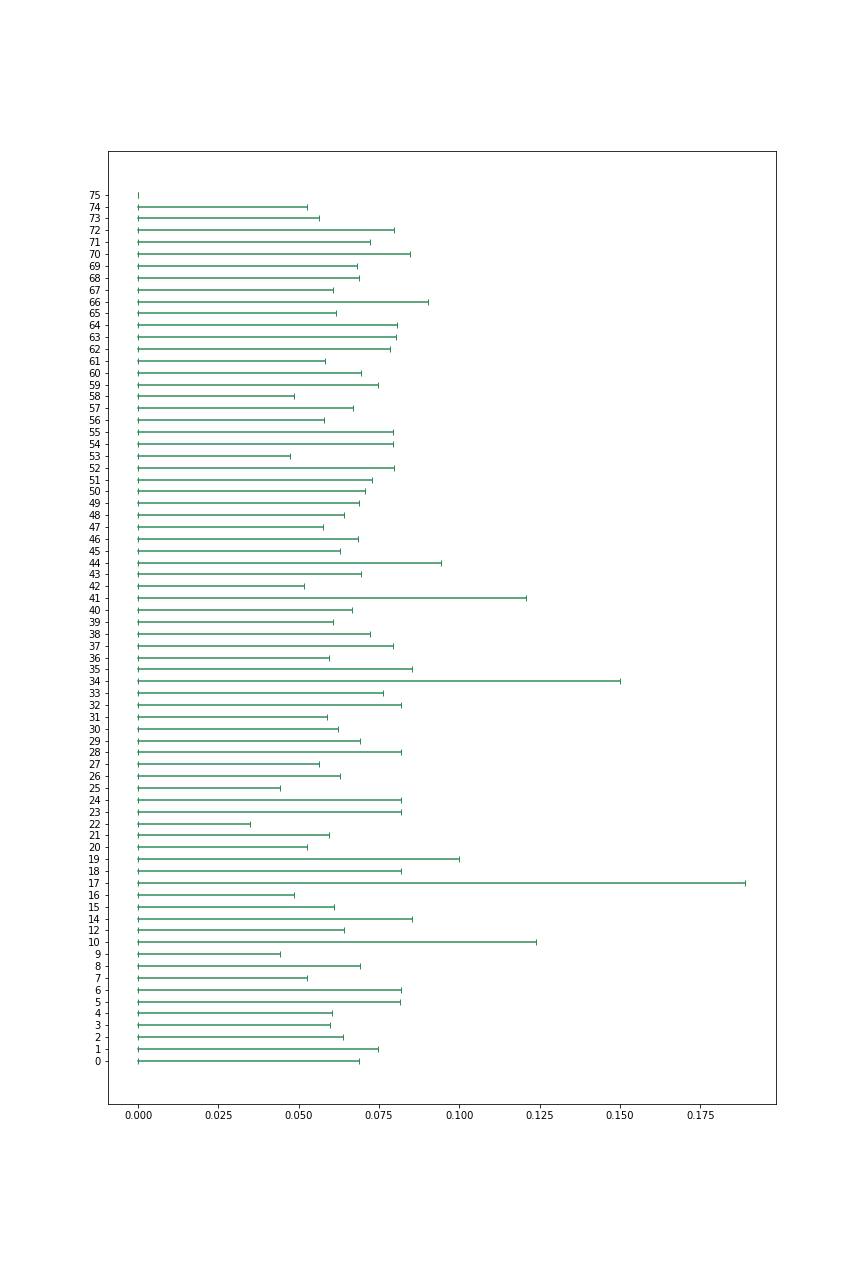
\includegraphics[scale=0.37]{pictures/all_cis_lim_alpha.png} %wrong name, right plot
    \caption[CIs for $\alpha$, limited. $\gamma=\kappa=1$]{Confidence intervals for $\alpha$ in the limited case of the box task with $\gamma=\kappa=1$ for each participant. Individual number 11 has a much higher value of the upper limit than the range of the axis here. }
    \label{fig:all_cis_alpha_lim}
\end{figure}

In Figure \ref{fig:all_cis_beta}, we have plotted all the confidence intervals for $\beta$ in the limited case. Again, we see that individual 11 has a large interval that spans beyond the axis here. Many of the intervals include zero. Having $\hb=0$ means that one does not feel any loss if the test terminates, although this is defined as a failed trial. We also see that most of the participants have upper limits below one, meaning that failed trials are not disastrous for most participants. 
\begin{figure}
    \centering
    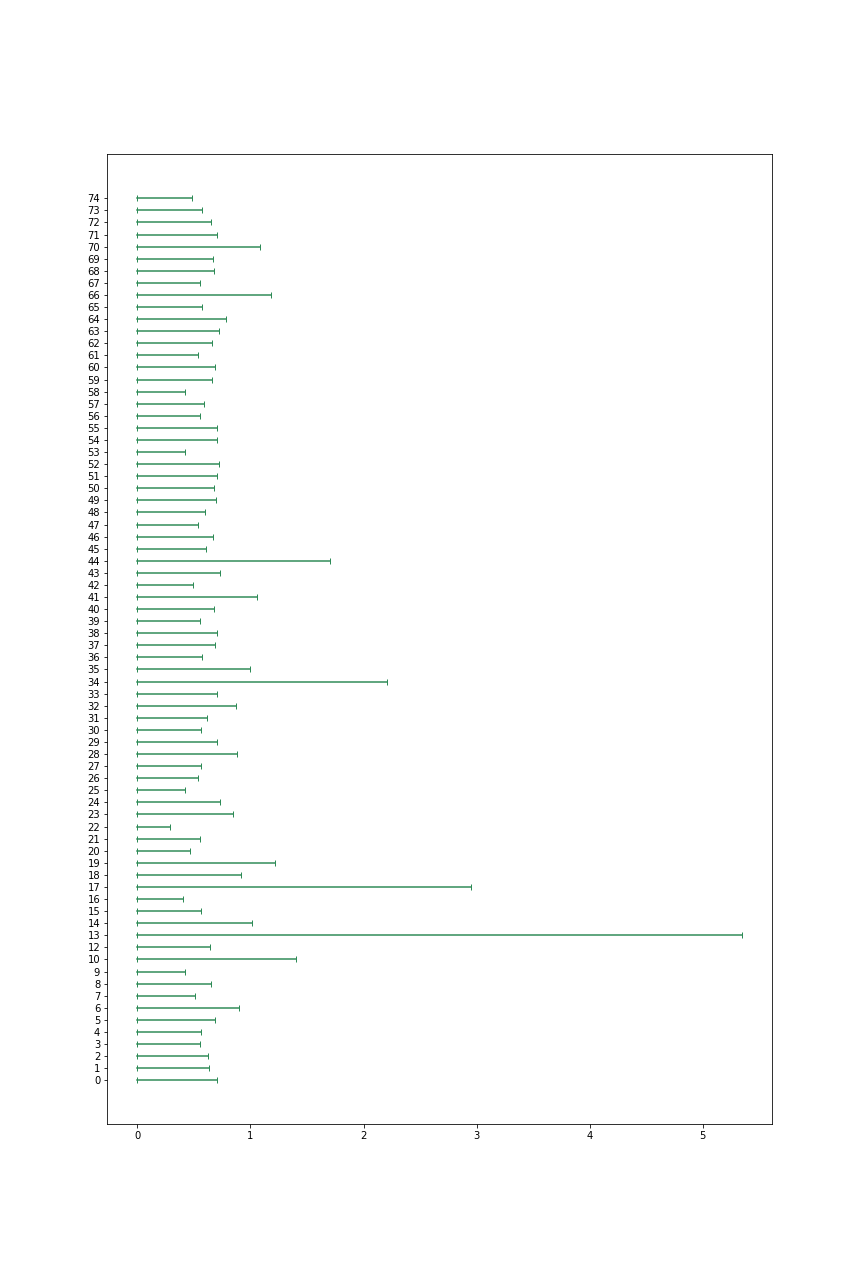
\includegraphics[scale=0.38]{pictures/all_cis_lim_beta.png}
    \caption[CIs for $\beta$, limited. $\gamma=\kappa=1$]{Confidence intervals for $\beta$ in the limited case of the box task with $\gamma=\kappa=1$ for each participant. As in Figure \ref{fig:all_cis_alpha_lim} participant 11 has a long interval.}
    \label{fig:all_cis_beta}
\end{figure}

We have also plotted the confidence interval for $\eta$ for each participant. This is shown in Figure \ref{fig:all_cis_eta_lim}. The CI for participant 70 is not included here as it is much higher than the range of the axis. There are only two CIs that include zero, the ones for participants 11 and 13. The rest of the intervals are above zero. That indicates that most participants make  choices with little expected loss, whereas individuals 11 and 13 might tend to make decisions with higher expected losses. Many participants have long intervals which might mean that there is uncertainty tied to their estimates. 
\begin{figure}
    \centering
    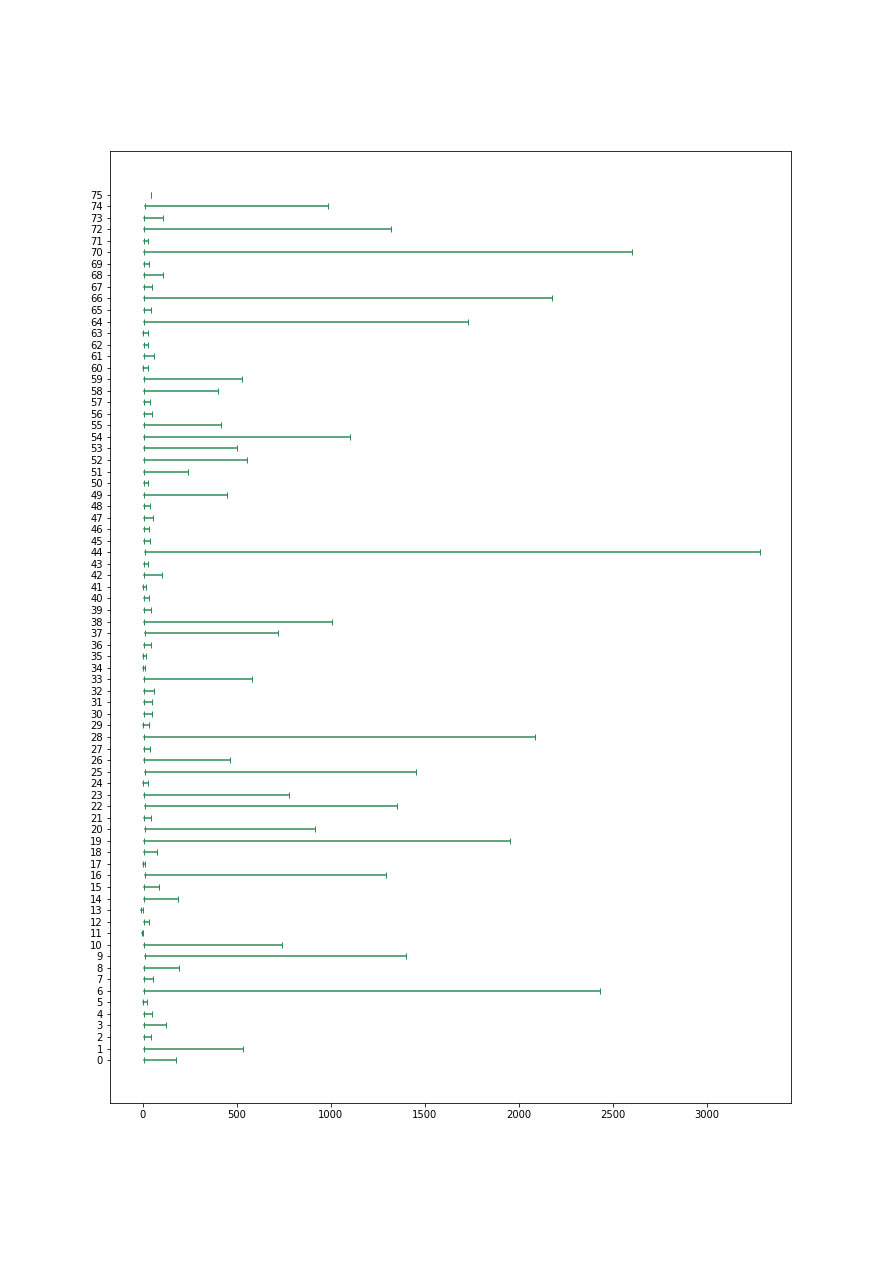
\includegraphics[scale=0.37]{pictures/all_cis_lim_eta.png}
    \caption[CIs for $\eta$, limited. $\gamma=\kappa=1$]{Confidence intervals for $\eta$ in the limited case of the box task with $\gamma=\kappa=1$ for each participant. Participant 70 has a too high CI to be included here.}
    \label{fig:all_cis_eta_lim}
\end{figure}


We have three participants where all of the confidence intervals have length zero. These are individuals 21, 70 and 75. As for individual 75 in the unlimited case, they have very high values of $\he$, which makes the probabilities of each of the decisions as seen in \eqref{probabilities_bootstrap} be approximately zero or approximately one. Thus, all the simulated decisions are the same as the decisions they have done. All of the 1000 MLEs are therefore the same, and finding the percentiles therefore give the same value as the MLEs. It should be noted that individual 75 has $\he=70.87$ as seen in \ref{mles_lim_person75}, which is far below the threshold value of 1000 that we defined for $\eta$. She has a quite high estimate of $\beta$, which makes the expected loss of opening the next box relatively high. Therefore, the expected losses differ considerably, and it takes a much lower value of $\he$ for the probabilities in \eqref{probabilities_bootstrap} to be approximately zero or one. Thus, $\he=70.87$ is a high value for individual number 75.


In Figures \ref{fig:all_cis_alpha_lim} and \ref{fig:all_cis_beta} we see that individual 11 has long confidence intervals for $\alpha$ and $\beta$. In Figure \ref{fig:ci_lim_a_b_person_11} we have plotted $\ha$ and $\hb$ of the 1000 bootstrap samples for individual 11 together with the confidence intervals for $\alpha$ and $\beta$.
We have zoomed in in that plot in Figure \ref{fig:ci_lim_a_b_person_11_zoomed}. Additionally, we have plotted the MLEs and the confidence intervals of $\alpha$ and $\eta$ in Figure \ref{fig:ci_lim_a_e_person_11} and zoomed in on that plot in Figure \ref{fig:ci_lim_a_e_person_11_zoomed}.
The confidence intervals are 
\begin{equation*}
    [\hat{\alpha}^{*(5)}_{1000},\hat{\alpha}^{*(95)}_{1000}] = [0.2935,649.1],
\end{equation*}
\begin{equation*}
    [\hb^{*(5)}_{1000},\hb^{*(95)}_{1000}] = [0,16.74]
\end{equation*}
and
\begin{equation*}
    [\hat{\eta}^{*(5)}_{1000},\hat{\eta}^{*(95)}_{1000}] = [-10.45,-0.0013].
\end{equation*}
We see also here that there are many high values of $\ha$, which again give long intervals that indicates an uncertain estimate of $\alpha$. Furthermore, there are some extreme values of $\hb$. The CI has upper limit at 16.74, which is quite high compared to the other participants. Thus, there are some uncertainty tied to the estimate of both $\alpha$ and $\beta$ for individual 11, indicating that this model is not a good fit. As discussed for individual 13 in the unlimited version, this might be because we assume Ideal Observer decisions when we find the expected losses of opening the next box. These decisions are not that relevant for participant 11 as she tends to make decisions with high expected losses. She actually chooses the colour that is in minority multiple times, meaning that she chooses the decisions with the highest expected loss. 
\begin{figure}
    \centering
    \begin{minipage}{0.48\textwidth}
        \centering
        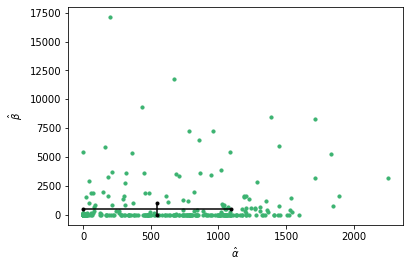
\includegraphics[scale=0.37]{pictures/ci_lim_a_b_person11.png}
        \caption{ci lim person 11}
        \label{fig:ci_lim_a_b_person_11}
    \end{minipage}\hfill
    \begin{minipage}{0.48\textwidth}
        \centering
        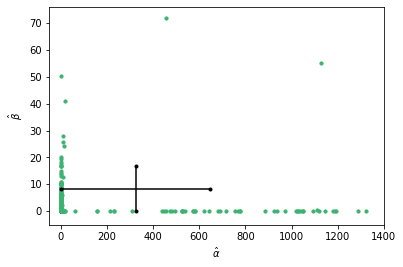
\includegraphics[scale=0.37]{pictures/ci_lim_a_b_person11_zoomed.png}
        \caption{ci lim person 11 zoomed}
        \label{fig:ci_lim_a_b_person_11_zoomed}
    \end{minipage}
\end{figure}

\begin{figure}
    \centering
    \begin{minipage}{0.48\textwidth}
        \centering
        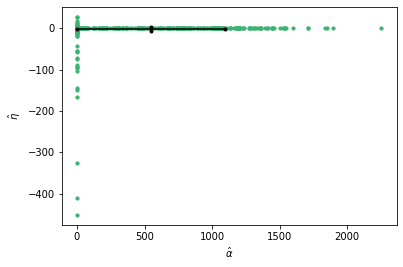
\includegraphics[scale=0.37]{pictures/ci_lim_a_e_person11.png}
        \caption[MLEs for $\alpha$ and $\beta$ for bootstrap samples individual 11, limited]{All of the MLEs for $\alpha$ and $\beta$ of the 1000 bootstrap samples plotted for individual number 11 in the limited case with $\gamma=\kappa=1$. The confidence intervals for the two parameters are also included.}
        \label{fig:ci_lim_a_e_person_11}
    \end{minipage}\hfill
    \begin{minipage}{0.48\textwidth}
        \centering
        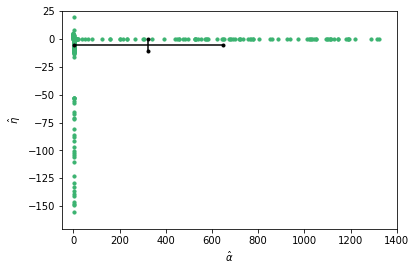
\includegraphics[scale=0.37]{pictures/ci_lim_a_e_person11_zoomed.png}
        \caption[MLEs for $\alpha$ and $\beta$ of bootstrap samples individual 11, unlimited, zoomed]{Here we have zoomed in on the bootstrap samples and confidence intervals that are plotted in Figure \ref{fig:ci_lim_a_e_person_11}. This is for individual number 11 in the limited case with $\gamma=\kappa=1$.}
        \label{fig:ci_lim_a_e_person_11_zoomed}
    \end{minipage}
\end{figure}

In Figure \ref{fig:ci_lim_b_e_person_11} we see $\hb$ and $\he$ of participant number 11 for the 1000 bootstrap samples plotted, and zoomed in Figure \ref{fig:ci_lim_b_e_person_11_zoomed}. We see that the whole interval for $\eta$ is below zero. This is a strong indicator that individual 11 makes many choices with high expected losses.
\begin{figure}
    \centering
    \begin{minipage}{0.48\textwidth}
        \centering
        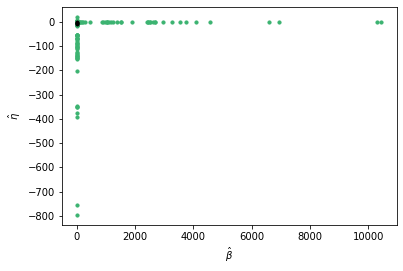
\includegraphics[scale=0.37]{pictures/ci_lim_b_e_person11.png}
        \caption[MLEs for $\beta$ and $\eta$ for bootstrap samples individual 11, limited]{All of the MLEs for $\beta$ and $\eta$ of the 1000 bootstrap samples plotted for individual number 11 in the limited case with $\gamma=\kappa=1$. The confidence intervals for the two parameters are also included.}
        \label{fig:ci_lim_b_e_person_11}
    \end{minipage}\hfill
    \begin{minipage}{0.48\textwidth}
        \centering
        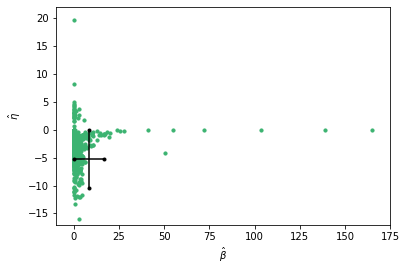
\includegraphics[scale=0.37]{pictures/ci_lim_b_e_person11_zoomed.png}
        \caption[MLEs for $\beta$ and $\eta$ of bootstrap samples individual 11, unlimited, zoomed]{Here we have zoomed in on the bootstrap samples and confidence intervals that are plotted in Figure \ref{fig:ci_lim_b_e_person_11}. This is for individual number 11 in the limited case with $\gamma=\kappa=1$.}
        \label{fig:ci_lim_b_e_person_11_zoomed}
    \end{minipage}
\end{figure}

In Figure \ref{fig:ci_lim_a_b_person40}, we have plotted the MLEs of $\alpha$ and $\beta$ for the 1000 bootstrap samples of individual 40 that is a more typical person. We see that $\ha$ and $\hb$ tend to not be zero at the same time, indicating that she gets some loss of opening boxes, but it differs whether the MLE is putting weight on $\alpha$ or $\beta$. In Figure \ref{fig:ci_lim_a_e_person_40} we have plotted all $\ha$ and $\he$ together, and zoomed in on that plot in Figure \ref{fig:ci_lim_a_e_person_40_zoomed}. Here we see that there are many high values of $\he$, and that the confidence interval is long. The values of $\hb$ and $\he$ are plotted in Figure \ref{fig:ci_lim_b_e_person_40} and we have zoomed in Figure \ref{fig:ci_lim_b_e_person_40_zoomed}. 
The confidence intervals are 
\begin{equation*}
    [\hat{\alpha}^{*(5)}_{1000},\hat{\alpha}^{*(95)}_{1000}] = [0,0.0665],
\end{equation*}
\begin{equation*}
    [\hb^{*(5)}_{1000},\hb^{*(95)}_{1000}] = [0,0.6763]
\end{equation*}
and
\begin{equation*}
    [\hat{\eta}^{*(5)}_{1000},\hat{\eta}^{*(95)}_{1000}] = [4.2926,31.287].
\end{equation*}
\begin{figure}
    \centering
    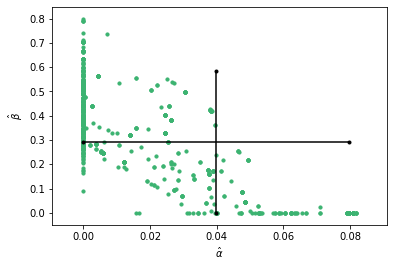
\includegraphics[scale=0.5]{pictures/ci_lim_a_b_person40.png}
    \caption[MLEs for $\alpha$ and $\beta$ for bootstrap samples individual 40, limited]{All of the MLEs for $\alpha$ and $\beta$ of the 1000 bootstrap samples plotted for individual number 40 in the limited case with $\gamma=\kappa=1$. The confidence intervals for the two parameters are also included.}
    \label{fig:ci_lim_a_b_person40}
\end{figure}
\begin{figure}
    \centering
    \begin{minipage}{0.48\textwidth}
        \centering
        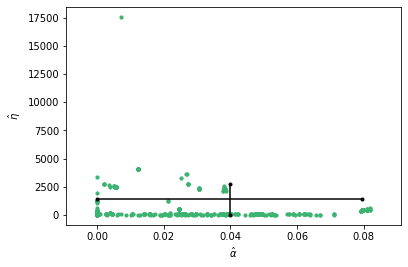
\includegraphics[scale=0.37]{pictures/ci_lim_a_e_person40.png}
        \caption[MLEs for $\alpha$ and $\eta$ for bootstrap samples individual 40, limited]{All of the MLEs for $\alpha$ and $\eta$ of the 1000 bootstrap samples plotted for individual number 40 in the limited case with $\gamma=\kappa=1$. The confidence intervals for the two parameters are also included.}
        \label{fig:ci_lim_a_e_person_40}
    \end{minipage}\hfill
    \begin{minipage}{0.48\textwidth}
        \centering
        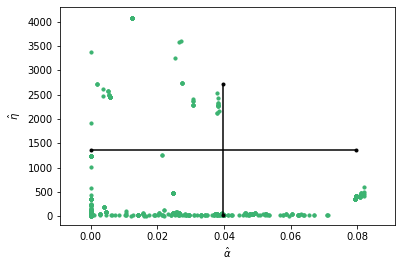
\includegraphics[scale=0.37]{pictures/ci_lim_a_e_person40_zoomed.png}
        \caption[MLEs for $\alpha$ and $\eta$ of bootstrap samples individual 40, unlimited, zoomed]{Here we have zoomed in on the bootstrap samples and confidence intervals that are plotted in Figure \ref{fig:ci_lim_a_e_person_40}. This is for individual number 11 in the limited case with $\gamma=\kappa=1$.}
        \label{fig:ci_lim_a_e_person_40_zoomed}
    \end{minipage}
\end{figure}
\begin{figure}
    \centering
    \begin{minipage}{0.48\textwidth}
        \centering
        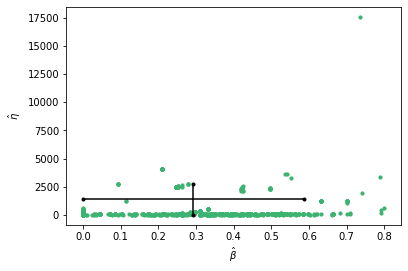
\includegraphics[scale=0.37]{pictures/ci_lim_b_e_person40.png}
        \caption[MLEs for $\beta$ and $\eta$ for bootstrap samples individual 40, limited]{All of the MLEs for $\beta$ and $\eta$ of the 1000 bootstrap samples plotted for individual number 40 in the limited case with $\gamma=\kappa=1$. The confidence intervals for the two parameters are also included.}
        \label{fig:ci_lim_b_e_person_40}
    \end{minipage}\hfill
    \begin{minipage}{0.48\textwidth}
        \centering
        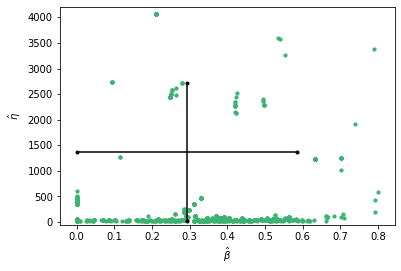
\includegraphics[scale=0.37]{pictures/ci_lim_b_e_person40_zoomed.png}
        \caption[MLEs for $\beta$ and $\eta$ of bootstrap samples individual 40, unlimited, zoomed]{Here we have zoomed in on the bootstrap samples and confidence intervals that are plotted in Figure \ref{fig:ci_lim_b_e_person_40}. This is for individual number 11 in the limited case with $\gamma=\kappa=1$.}
        \label{fig:ci_lim_b_e_person_40_zoomed}
    \end{minipage}
\end{figure}



We have now looked at the results when we have a uniform prior, thus that $\gamma=\kappa =1$. The next we will do is looking at how the results are influenced by a different prior. Thus, we look at the sensitivity of the hyperparameters $\gamma$ and $\kappa$.




\section{Sensitivity to Hyperparameters}
The results we have discussed so far have all been for a uniform prior of $\Theta$. 
Recall that $\Theta$ is the success probability in the Bernoulli distribution we have for the $X_i$'s, that are the colours of the boxes as described in \eqref{def_of_Xi}. Later we conditioned on there not being six blue and six red boxes. We have a beta prior for $\Theta$ with hyperparameters $\gamma$ and $\kappa$, as seen in \eqref{theta_with_beta_prior}. As we can see in Figure \ref{fig:pdf_beta_distr}, having $\gamma=\kappa=1$ is the same as having a uniform prior for $\Theta$. We will now have a look at how the results are affected by having a different prior. 

As discussed in Chapter \ref{section_notation}, the participants are told that one of the colours always is in majority, such that one might think that the probability that there are more of one of the colours is higher than the probability that there are six of each of the colours. Thus, we want a prior more like the purple or orange lines in Figure \ref{fig:pdf_beta_distr}. We choose the purple line where $\gamma=\kappa=0.5$.

With the new prior for $\Theta$, we have done the same as for the uniform prior. That is, we have found MLEs for all of the parameters and confidence intervals tied to each of them.

\subsection{Unlimited}
When we look at the sensitivity to hyperparameters, we start with the results for the unlimited version.

In Figure \ref{fig:sensitivity_mls_unlim} we have plotted all the MLEs for both priors. The green dots are the MLEs in the model with the uniform prior for $\Theta$, and the orange points are the MLEs in the model with the new prior.
We see that the participants that had extreme values with the uniform priors, still have extreme values with the new prior, but the values differ considerably. The highest value of $\he$ is remarkably lower, but it is still above that threshold value we defined for $\eta$. This might be because of the flat log likelihood function, making the high estimates of $\eta$ quite uncertain, as discussed in Chapter \ref{chapter:mles}. Thus, the big change in $\he$ might not be because of the new prior, but because of the numerical optimisation. 
If we zoom in in the plot in Figure \ref{fig:sensitivity_mls_unlim}, as we have done in Figure \ref{fig:sensitivity_mls_unlim_zoom1}, we see that the participants with high, but not extreme, values of $\he$ or $\ha$ have shifted their MLEs substantially. 
However, zooming even more, as in Figure \ref{fig:sensitivity_mls_unlim_zoom2}, we see that the MLEs of the participants that do not have extreme values are shifted a little, but not considerably, with some exceptions. All the participant that did not have $\ha=0$ from before, has shifted the values of $\ha$ closer to zero with the new prior. 
This is because with $\gamma=\kappa=0.5$, the model put more weight on the colours of the boxes that are opened. If, for example, many of the opened boxes are blue, then the probability that blue is the majority colour is higher in the model with the new prior. That means that if a participant chooses early, these decisions are more compatible with the model with the lower values of $\gamma$  and $\kappa$. 
Thus, it is reasonable that we have smaller values of $\ha$ for the new model. 
Most of the participants that have $\ha=0$ in the first model have the same in the alternative model. We also see that most of these participants have the same or about the same value of $\he$, perhaps slightly shifted upwards, with the new prior. For the other participants there are, with some exceptions, no huge differences in the values of $\he$, considering the scale we have the values on. Some participants get higher values of $\he$ and others get lower values without there being any clear pattern. 
\begin{figure}
    \centering
    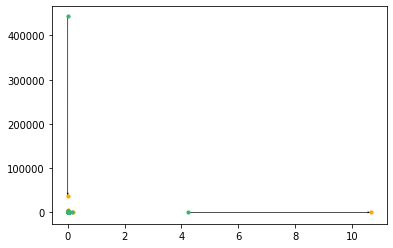
\includegraphics[scale=0.7]{pictures/Sensitivity/mles_unlim.png}
    \caption[MLEs for prior with $\gamma=\kappa=1$ and $\gamma=\kappa=0.5$, unlimited]{
    Maximum likelihood estimates in the unlimited version of the box task. The green dots represent MLEs where we have a uniform prior for $\Theta$, that is, $\gamma=\kappa=1$. The orange dots are the MLEs where $\gamma=\kappa=0.5$.}
    \label{fig:sensitivity_mls_unlim}
\end{figure}
\begin{figure}
    \centering
    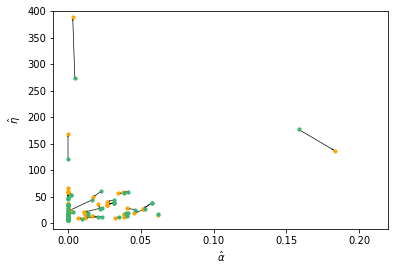
\includegraphics[scale=0.8]{pictures/Sensitivity/mles_unlim_zoom1.png}
    \caption[Zoomed in on the MLEs in Figure \ref{fig:sensitivity_mls_unlim}]{MLEs for two different priors in the unlimited case of the box task. This is the same plot as in Figure \ref{fig:sensitivity_mls_unlim} zoomed in.}
    \label{fig:sensitivity_mls_unlim_zoom1}
\end{figure}
\begin{figure}
    \centering
    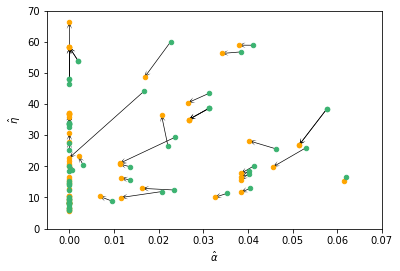
\includegraphics[scale=0.8]{pictures/Sensitivity/mles_unlim_zoom2.png}
    \caption[Zoomed in on the MLEs in Figure \ref{fig:sensitivity_mls_unlim_zoom1}]{The plot of MLEs in Figure \ref{fig:sensitivity_mls_unlim_zoom1} zoomed.}
    \label{fig:sensitivity_mls_unlim_zoom2}
\end{figure}



In Figure \ref{fig:sensitivity_unlim_cis_alpha} we see the confidence intervals for $\alpha$. The green lines are the CIs we found earlier with the uniform prior, and the orange lines represent the CIs when we have the beta prior for $\Theta$ with $\gamma=\kappa=0.5$. As for the MLEs we see that the confidence intervals are close to each other. Many of the upper limits are slightly shifted to the left, with some exceptions. (jeg vet neste ikke hva jeg skal si? de er jo veldig like?) Again, we see that the interval of individual 13 is long, such that the upper limit is outside of this plot. These upper limits are also quite similar. 
\begin{figure}
    \centering
    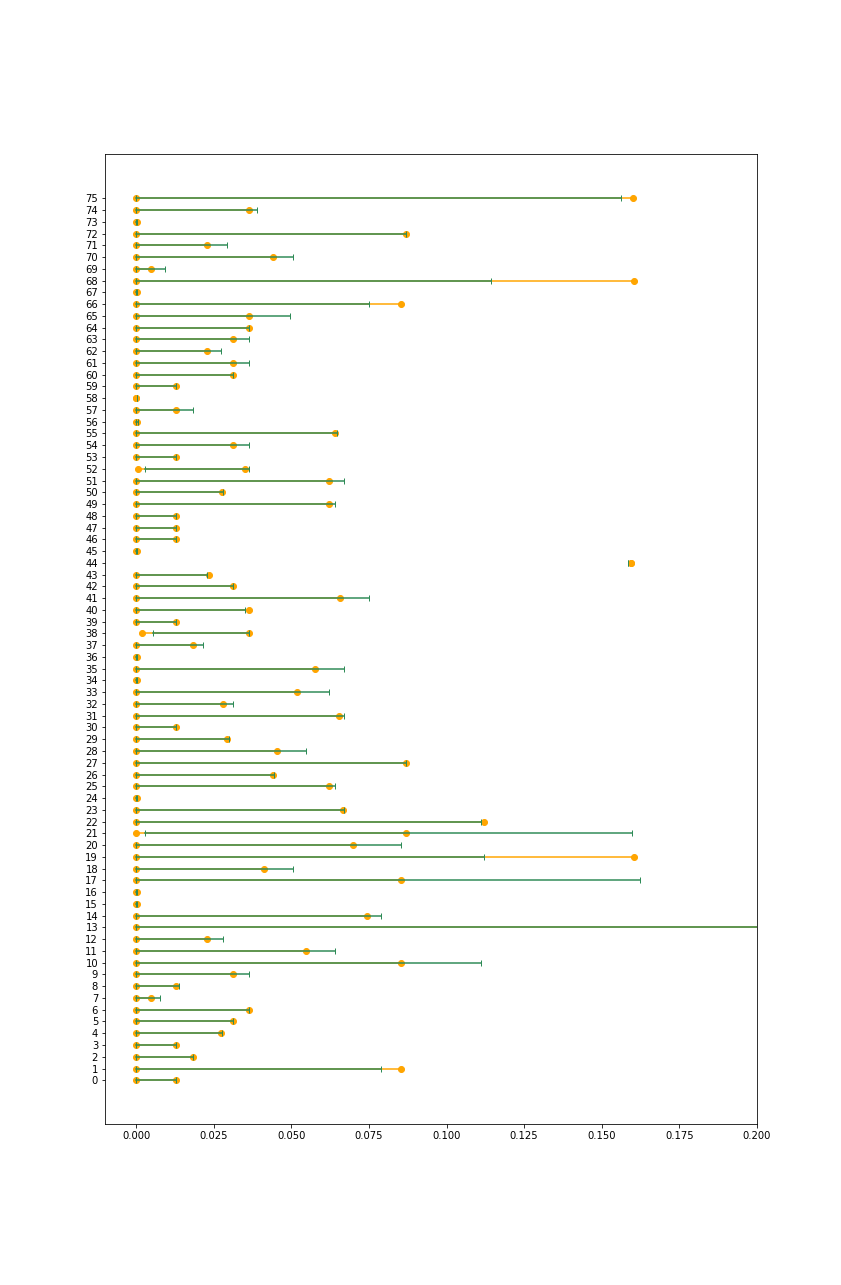
\includegraphics[scale=0.37]{pictures/Sensitivity/ci_unlim_alpha.png}
    \caption[CIs for $\alpha$ for all participants with two different priors, unlimited]{
    Confidence intervals for $\alpha$ for all of the 76 participants in the unlimited version of the box task. The green intervals represent the situation where we have a uniform prior for $\Theta$, that is, $\gamma=\kappa=1$. The orange lines are the intervals for a prior where $\gamma=\kappa=0.5$.}
    \label{fig:sensitivity_unlim_cis_alpha}
\end{figure}


Figure \ref{fig:sensitivity_unlim_cis_eta} displays the confidence intervals for $\eta$ for each participant. We also have here that the orange lines are the CIs in the case with the new prior and the green lines are the CIs we found in the case with the uniform prior. In Figure \ref{fig:sensitivity_unlim_cis_eta_zoomed} we have zoomed in closer to zero to get a better view of the participants we lower values of $\he$. The confidence intervals for $\eta$ differ more than the intervals for $\alpha$. 
Some of the new intervals are shorter and others are longer than the old ones, without there being any clear pattern of which intervals that is. Some intervals are slightly shifted to the right. At least the intervals that are longer than the original intervals. There, it is mostly the upper limits that are higher than the original, and the new lower limits are often close to the old ones. 
However, these higher upper limits might be because of the flat log likelihood function as discussed in Chapter \ref{chapter:mles}. 
\begin{figure}
    \centering
    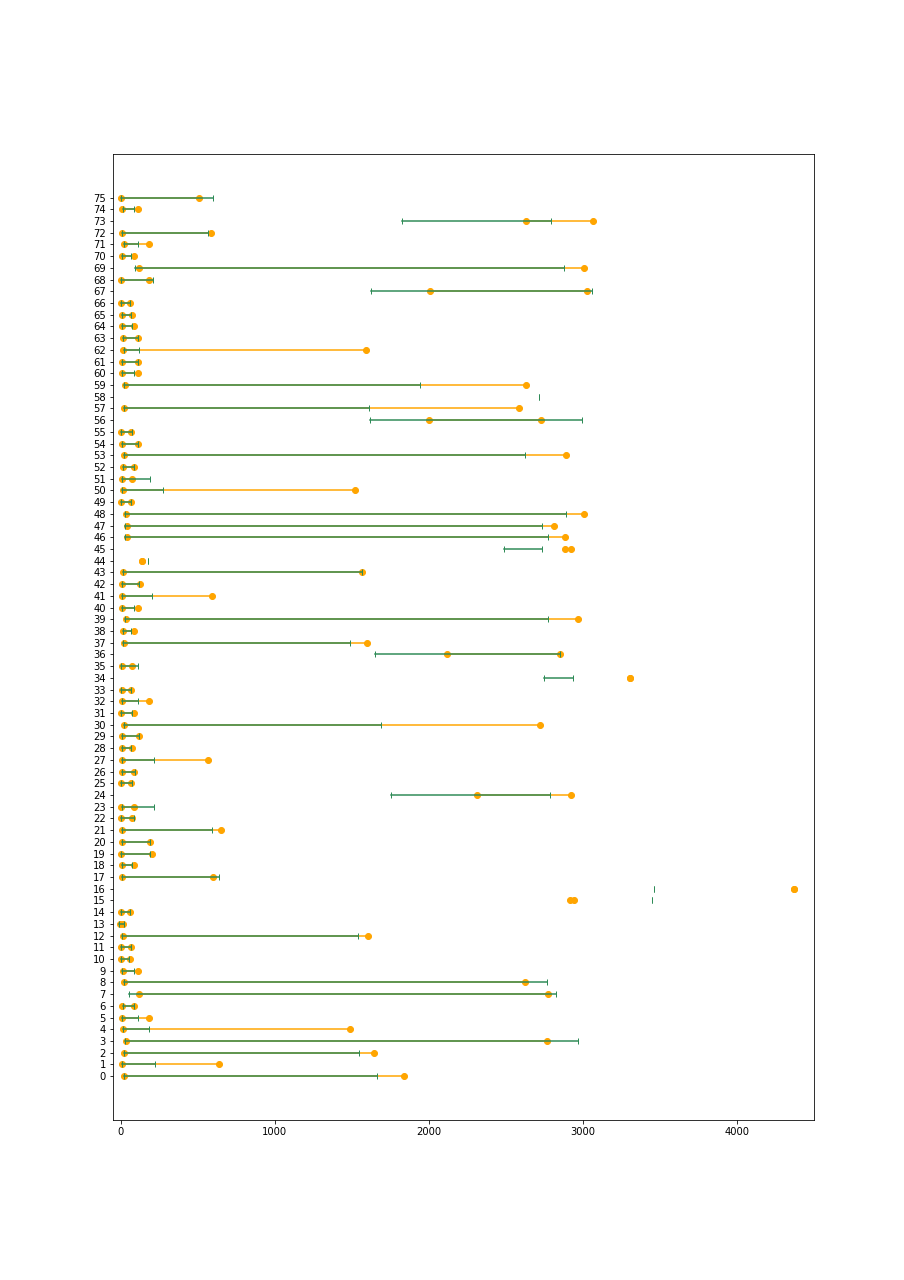
\includegraphics[scale=0.36]{pictures/Sensitivity/ci_unlim_eta.png}
    \caption[CIs for $\eta$ for all participants with two different priors, unlimited]{
    Confidence intervals for $\eta$ for all of the 76 participants in the unlimited version of the box task. The green intervals represent the situation where we have a uniform prior for $\Theta$, that is, $\gamma=\kappa=1$. The orange lines are the intervals for a prior where $\gamma=\kappa=0.5$.}
    \label{fig:sensitivity_unlim_cis_eta}
\end{figure}
\begin{figure}
    \centering
    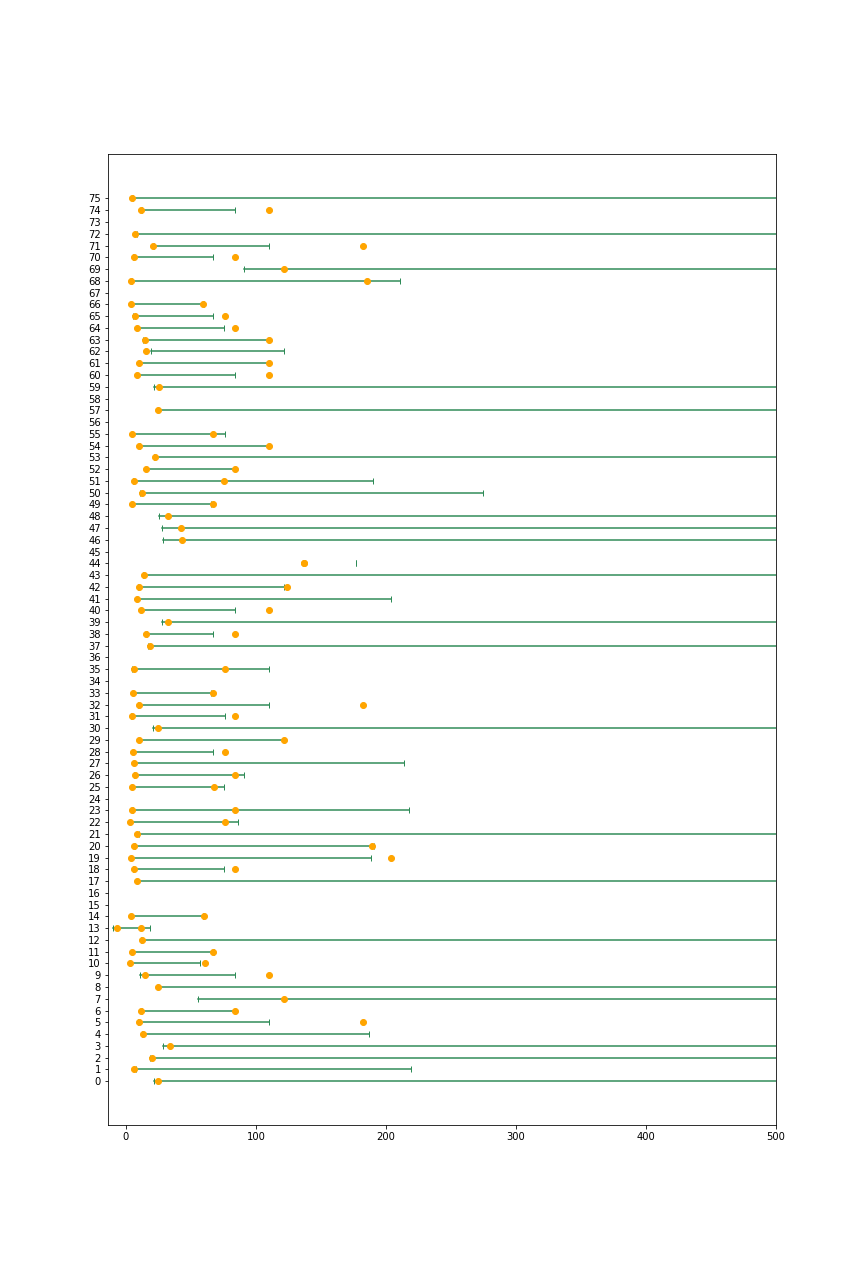
\includegraphics[scale=0.36]{pictures/Sensitivity/ci_unlim_eta_zoomed.png}
    \caption[CIs for $\eta$, unlimited. Zoomed]{The plot in Figure \ref{fig:sensitivity_unlim_cis_eta} zoomed.}
    \label{fig:sensitivity_unlim_cis_eta_zoomed}
\end{figure}







%the model will now predict that they choose earlier, thus, they are more consisten with the best choices as in general people tend to choose early, at least earlier than an IO (or earlier than they would need to do if they would choose the alternative with the least exp loss). 


%note to self: gamma and kappa smaller give more 'weight' to the colour of the boxes that are oepned. hence, we choose earlier because the prob that blue is majority is bigger here than for unif if one blue box is opened. 

\subsection{Limited}
We continue with looking at the estimates and confidence intervals using a new prior for $\Theta$ in the limited case of the box task. 

In the previous results where we have a uniform prior, we have that all the $\ha$ are zero except for two. In Figure \ref{fig:sensitivity_mles_lim_a_e} we have plotted both the new and the old estimates of $\alpha$ and $\eta$. The green dots are the estimates for the model with the uniform prior and the orange are the new estimates with the beta prior having hyperparameters $\gamma=\kappa=0.5$. 
We see that all $\ha$ that were zero from before are still zero with the new prior. The two participants, individuals 11 and 13 that have the high values of $\ha$ get higher values of $\ha$. Their values of $\he$ are slightly higher with the new prior. 
There are three participants that had values of $\ha$ slightly higher than zero, that with the new prior have $\ha=0$. 
Most participants get lower value of $\he$ with the non-uniform prior. Most of the values are only shifted a little downwards with the exception of some that get a huge difference in the values. These are participants that have huge values of $\he$ from before with the uniform prior. We discussed earlier that the log likelihood function is flat for high values of $\eta$, and that the stopping criterion in the optimisation can be met several places when $\eta$ is high. This might be the reason for the big change in the value of $\he$. 
A few participants get higher values of $\he$, but if the values are higher it is not by a lot. 
\begin{figure}
    \centering
    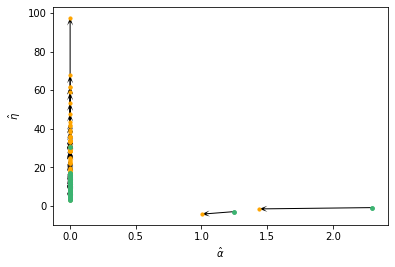
\includegraphics[scale=0.8]{pictures/Sensitivity/mles_lim_a_e.png}
    \caption[MLEs of $\alpha$ and $\eta$ for prior with $\gamma=\kappa=1$ and $\gamma=\kappa=0.5$, limited]{
    Maximum likelihood estimates of $\alpha$ and $\eta$ in the limited version of the box task. The green dots represent MLEs where we have a uniform prior for $\Theta$, that is, $\gamma=\kappa=1$. The orange dots are the MLEs where $\gamma=\kappa=0.5$.}
    \label{fig:sensitivity_mles_lim_a_e}
\end{figure}

In addition to this, we have plotted the MLEs for $\alpha$ and $\beta$ together in Figure \ref{fig:sensitivity_mles_lim_a_b}. We see also here participants 11 and 13 with the high values of $\ha$. Their values of $\hb$ were zero with the uniform prior, and stay zero with the new prior. We also see one participant that increases the value of $\hb$ by a lot. This is individual number 75. Recall that this is the participant that has confidence intervals of length zero because of the high value of $\he$. Her MLEs are given in \eqref{mles_lim_person75}. The log likelihood function is also quite flat for big values of $\alpha$ or $\beta$, meaning that the same argument for high differences in $\he$ holds for $\hb$ as well.  
\begin{figure}
    \centering
    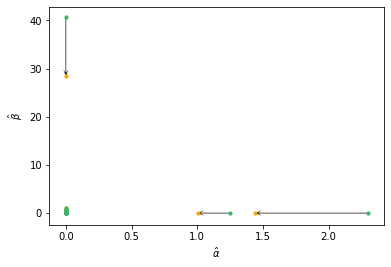
\includegraphics[scale=0.8]{pictures/Sensitivity/mles_lim_a_b.png}
    \caption[MLEs of $\alpha$ and $\beta$ for prior with $\gamma=\kappa=1$ and $\gamma=\kappa=0.5$, limited]{
    Maximum likelihood estimates of $\alpha$ and $\beta$ in the limited version of the box task. The green dots represent MLEs where we have a uniform prior for $\Theta$, that is, $\gamma=\kappa=1$. The orange dots are the MLEs where $\gamma=\kappa=0.5$.}
    \label{fig:sensitivity_mles_lim_a_b}
\end{figure}

As so many of the values of $\ha$ are zero, zooming in on Figure \ref{fig:sensitivity_mles_lim_a_b} will give little information. We therefore go straight to the plot for $\hb$ and $\he$, that is shown in Figure \ref{fig:sensitivity_mles_lim_b_e}. Here, we again see participant 75 that gets a much higher $\hb$. She gets a smaller value of $\he$, but again, that might be because of the flat log likelihood function. 
\begin{figure}
    \centering
    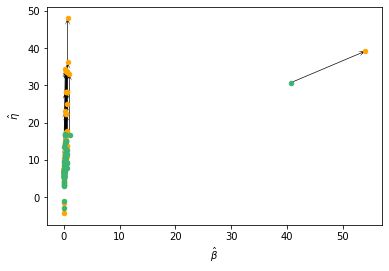
\includegraphics[scale=0.8]{pictures/Sensitivity/mles_lim_b_e.png}
    \caption[MLEs of $\beta$ and $\eta$ for prior with $\gamma=\kappa=1$ and $\gamma=\kappa=0.5$, limited]{
    Maximum likelihood estimates of $\beta$ and $\eta$ in the limited version of the box task. The green dots represent MLEs where we have a uniform prior for $\Theta$, that is, $\gamma=\kappa=1$. The orange dots are the MLEs where $\gamma=\kappa=0.5$.}
    \label{fig:sensitivity_mles_lim_b_e}
\end{figure}

If we zoom in as in Figure \ref{fig:sensitivity_mles_lim_b_e_zoomed}, we see that most participants, with some exceptions, get smaller values of both $\hb$ and $\he$. All the participants that had $\hb=0$ with the uniform prior still has that with the non-uniform prior. In fact, more participants have $\hb=0$ now than with the uniform prior. All the other participants, except participant 75, get slightly smaller values of $\hb$.
If there for example are many red boxes that are opened, we have that the probability that red is the majority colour is higher with the non-uniform prior than with the uniform. Thus, the expected loss of choosing red as the majority colour is lower now than it was with the uniform prior. Then, if one chooses majority colour early, the expected loss is closer to the lowest expected loss. Therefore, one are not to the same degree interpreted as being afraid of the test terminating when choosing early. Thus, many of the values of $\hb$ are lower here. 
%Many of the participants chooses what they think is the majority colour early, meaning that they choose when few boxes are opened. With the new prior giving lower expected losses of choosing majority colour early, that means that the participants make decisions closer to the decision that has the lowest expected loss. Thus, we get higher values of $\he$ if we use the new prior with $\gamma=\kappa=0.5$.
\begin{figure}
    \centering
    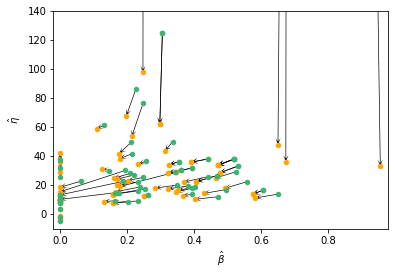
\includegraphics[scale=0.8]{pictures/Sensitivity/mles_lim_b_e_zoomed.png}
    \caption[MLEs of $\beta$ and $\eta$, zoomed]{The plot in Figure \ref{fig:sensitivity_mles_lim_b_e}, zoomed.}
    \label{fig:sensitivity_mles_lim_b_e_zoomed}
\end{figure}

In general, we get smaller values of all of the three parameters, with some exceptions, with the non-uniform prior for $\Theta$.


Intervsl for $\alpha$:
\begin{figure}
    \centering
    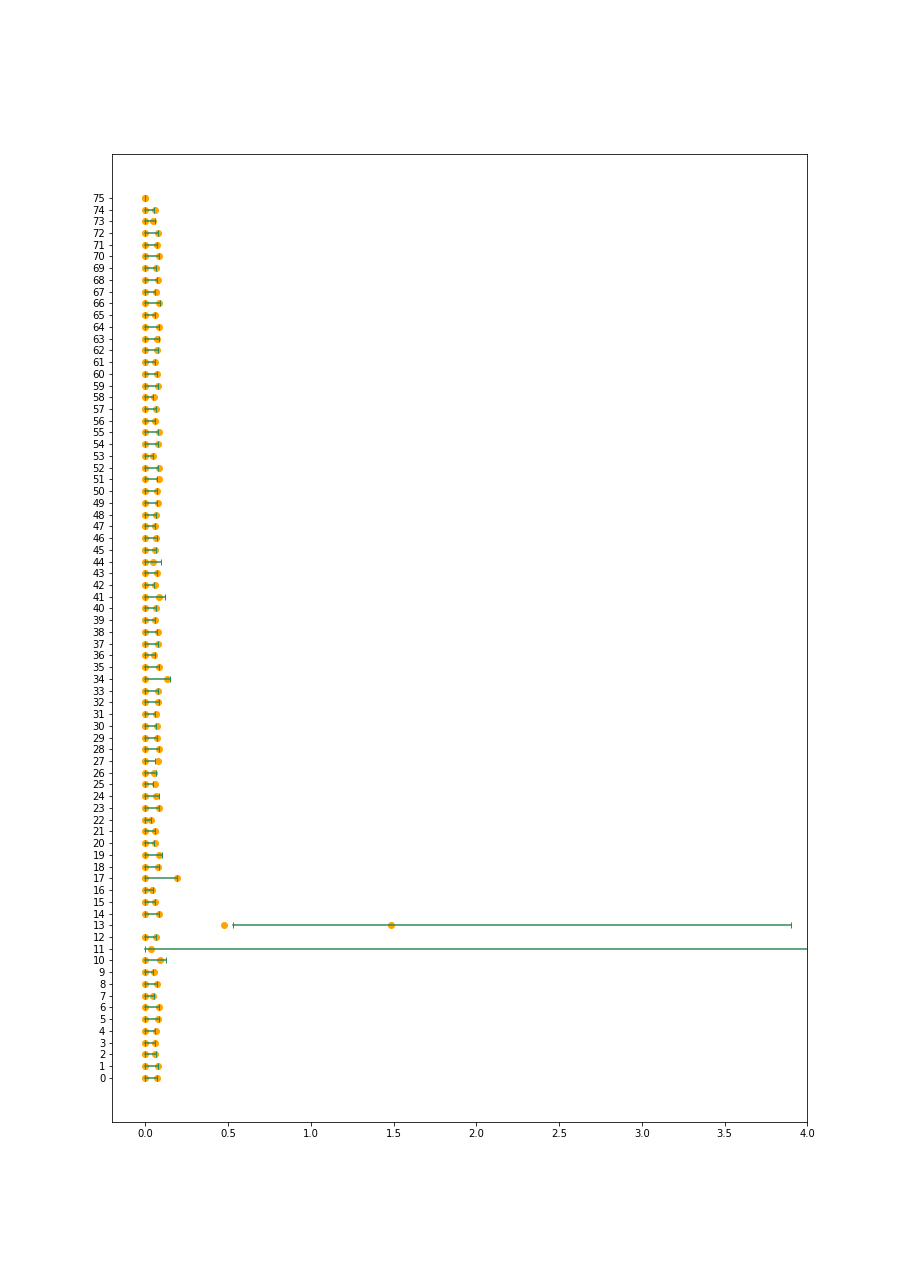
\includegraphics[scale=0.38]{pictures/Sensitivity/ci_lim_alpha_zoom1.png}
    \caption[CIs for $\alpha$ for all participants with two different priors, limited]{Confidence intervals for $\alpha$ for all of the 76 participants in the limited version of the box task. The green intervals represent the situation where we have a uniform prior for $\Theta$, that is, $\gamma=\kappa=1$. The orange lines are the intervals for a prior where $\gamma=\kappa=0.5$.}
    \label{fig:sensitivity_ci_lim_alpha_zoom1}
\end{figure}


zoomed even more in Appendix \ref{appendix_CIs}. and a plot including the whole interval for 11 is also included there.


\begin{figure}
    \centering
    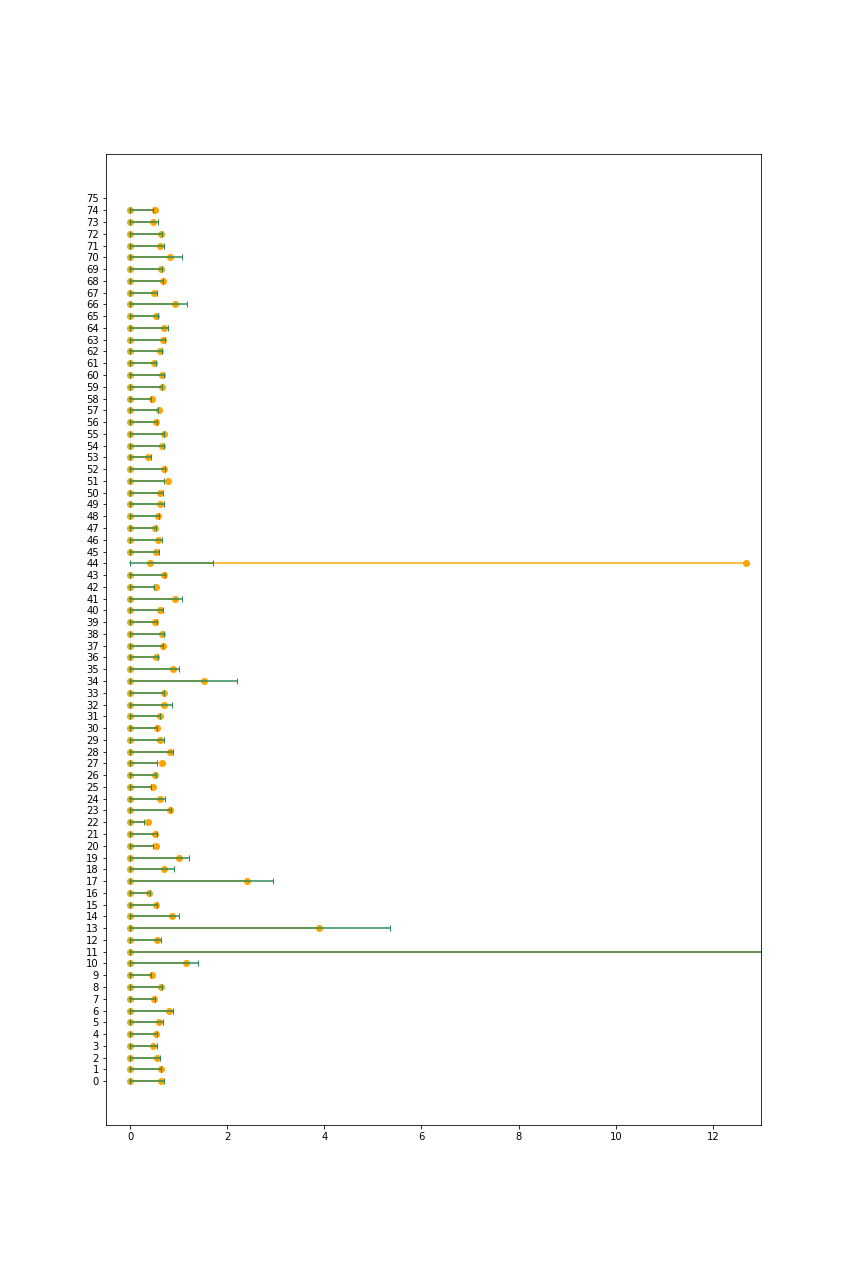
\includegraphics[scale=0.37]{pictures/Sensitivity/ci_lim_beta_zoom1.png}
    \caption[CIs for $\beta$ for all participants with two different priors, limited]{Confidence intervals for $\beta$ for all of the 76 participants in the limited version of the box task. The green intervals represent the situation where we have a uniform prior for $\Theta$, that is, $\gamma=\kappa=1$. The orange lines are the intervals for a prior where $\gamma=\kappa=0.5$.}
    \label{fig:sensitivity_ci_lim_beta_zoom}
\end{figure}

about cis for eta:
person 70 actually getting an interval here. 
\begin{figure}
    \centering
    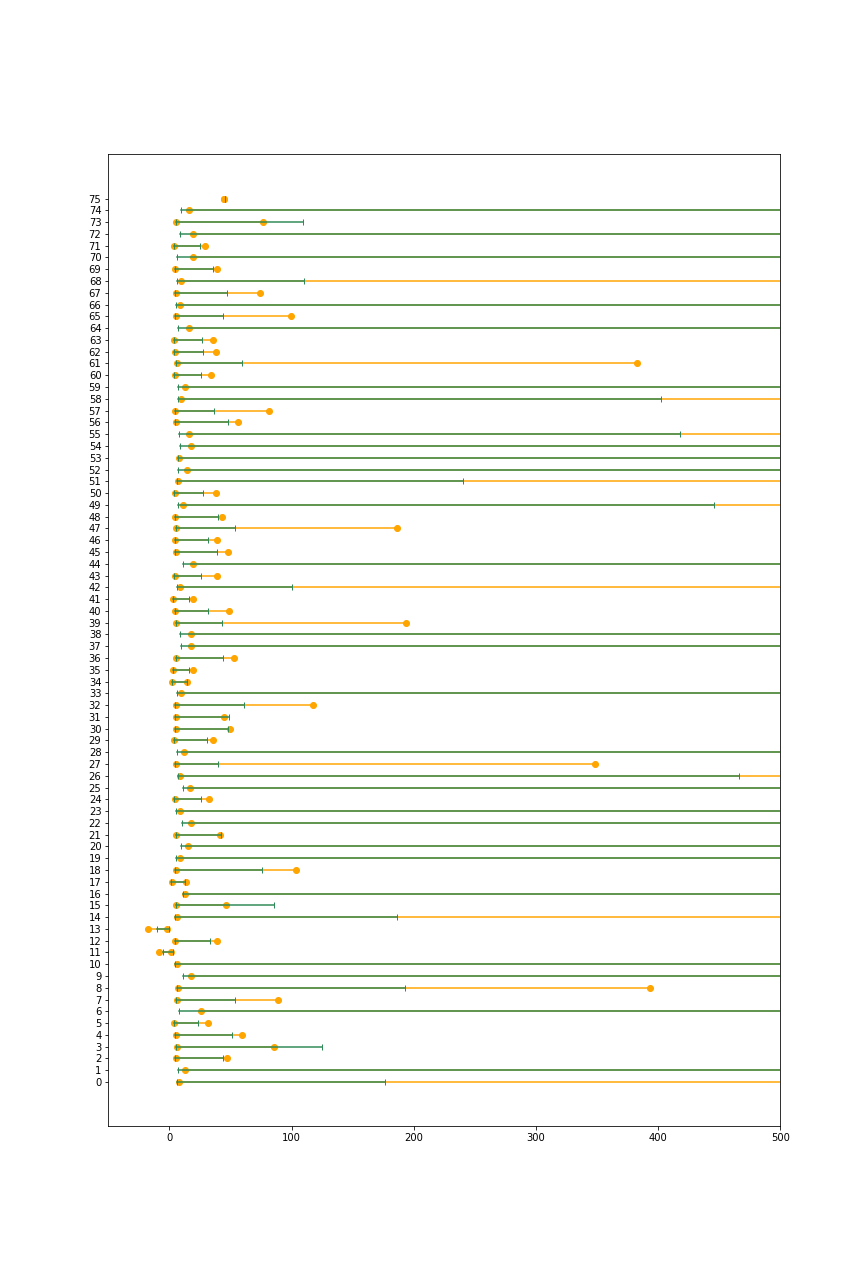
\includegraphics[scale=0.37]{pictures/Sensitivity/ci_lim_eta_zoomed.png}
    \caption[CIs for $\eta$ for all participants with two different priors, limited]{Confidence intervals for $\eta$ for all of the 76 participants in the limited version of the box task. The green intervals represent the situation where we have a uniform prior for $\Theta$, that is, $\gamma=\kappa=1$. The orange lines are the intervals for a prior where $\gamma=\kappa=0.5$. The old interval for person 70 is a scalar that has value 23851.9, thus it is outside the rage of this plot.}
    \label{fig:sensitivity_ci_lim_eta}
\end{figure}